%----------
%   IMPORTANTE
%----------

% Si nunca has utilizado LaTeX es conveniente que aprendas una serie de conceptos básicos antes de utilizar esta plantilla. Te aconsejamos que leas previamente algún tutorial (puedes encontar muchos en Internet).

% Esta plantilla está basada en las recomendaciones de la guía "Trabajo fin de Grado: Escribir el TFG", que encontrarás en http://uc3m.libguides.com/TFG/escribir
% contiene recomendaciones de la Biblioteca basadas principalmente en estilos APA e IEEE, pero debes seguir siempre las orientaciones de tu Tutor de TFG y la normativa de TFG para tu titulación.

% Encontrarás un ejemplo de TFG realizado con esta misma plantilla en la carpeta "_ejemplo_TFG_2019". Consúltalo porque contiene ejemplos útiles para incorporar tablas, figuras, listados de código, bibliografía, etc.


%----------
%	CONFIGURACIÓN DEL DOCUMENTO
%----------

% Definimos las características del documento y añadimos una serie de paquetes (\usepackage{package}) que agregan funcionalidades a LaTeX.

\documentclass[12pt]{report} %fuente a 12pt


% MÁRGENES: 2,5 cm sup. e inf.; 3 cm izdo. y dcho.
\usepackage[
a4paper,
vmargin=2.5cm,
hmargin=3cm
]{geometry}


% INTERLINEADO: Estrecho (6 ptos./interlineado 1,15) o Moderado (6 ptos./interlineado 1,5)
\renewcommand{\baselinestretch}{1.15}
\parskip=6pt

% DEFINICIÓN DE COLORES para portada y listados de código
\usepackage[table]{xcolor}
\definecolor{azulUC3M}{RGB}{0,0,102}
\definecolor{gray97}{gray}{.97}
\definecolor{gray75}{gray}{.75}
\definecolor{gray45}{gray}{.45}
\definecolor{tables}{RGB}{222,222,218}
\definecolor{anPlanif}{RGB}{255,196,29}
\definecolor{impPlanif}{RGB}{149,184,234}
\definecolor{resPlanif}{RGB}{235,118,113}
\definecolor{evalPlanif}{RGB}{220,137,174}
\definecolor{mantPlanif}{RGB}{190,190,190}
\definecolor{White}{RGB}{255,255,255}

% Soporte para GENERAR PDF/A --es importante de cara a su inclusión en e-Archivo porque es el formato óptimo de preservación y a la generación de metadatos, tal y como se describe en http://uc3m.libguides.com/ld.php?content_id=31389625. En la carpeta incluímos el archivo plantilla_tfg_2017.xmpdata en el que puedes incluir los metadatos que se incorporarán al archivo PDF cuando lo compiles. Ese archivo debe llamarse igual que tu archivo .tex. Puedes ver un ejemplo en esta misma carpeta.
\usepackage[a-1b]{pdfx}

% ENLACES
\usepackage{hyperref}
\hypersetup{colorlinks=true,
	linkcolor=black, % enlaces a partes del documento (p.e. índice) en color negro
	urlcolor=blue} % enlaces a recursos fuera del documento en azul

% EXPRESIONES MATEMATICAS
\usepackage{amsmath,amssymb,amsfonts,amsthm}

\usepackage{txfonts} 
\usepackage[T1]{fontenc}
\usepackage[utf8]{inputenc}

\usepackage{graphicx}
\usepackage{caption}

% simbolo euro
\usepackage{eurosym}

\usepackage[spanish, es-tabla]{babel} 
\usepackage[babel, spanish=spanish]{csquotes}
\AtBeginEnvironment{quote}{\small}

% diseño de PIE DE PÁGINA
\usepackage{fancyhdr}
\pagestyle{fancy}
\fancyhf{}
\renewcommand{\headrulewidth}{0pt}
\rfoot{\thepage}
\fancypagestyle{plain}{\pagestyle{fancy}}

% Glosario
\usepackage[nonumberlist]{glossaries}
% \usepackage[acronym, nonumberlist, section]{glossaries}
% \newglossary{lista-abreviaturas}{Lista de abreviaturas}
\makeglossaries

% \input{contenido/previo/04-Abreviaturas} %%%%%%%%%%%%%%%%%%%%%%%%%%%%%%%%%%%%%%%%%%%%%%%%%%%%%%%%%%%%%%%%
% \input{contenido/previo/05-Glosario}

% DISEÑO DE LOS TÍTULOS de las partes del trabajo (capítulos y epígrafes o subcapítulos)
\usepackage{titlesec}
\usepackage{titletoc}
\titleformat{\chapter}[block]
{\large\bfseries\filcenter}
{\thechapter.}
{5pt}
{\MakeUppercase}
{}
\titlespacing{\chapter}{0pt}{0pt}{*3}
\titlecontents{chapter}
[0pt]                                               
{}
{\contentsmargin{0pt}\thecontentslabel.\enspace\uppercase}
{\contentsmargin{0pt}\uppercase}                        
{\titlerule*[.7pc]{.}\contentspage}                 

\titleformat{\section}
{\bfseries}
{\thesection.}
{5pt}
{}
\titlecontents{section}
[5pt]                                               
{}
{\contentsmargin{0pt}\thecontentslabel.\enspace}
{\contentsmargin{0pt}}
{\titlerule*[.7pc]{.}\contentspage}

\titleformat{\subsection}
{\normalsize\bfseries}
{\thesubsection.}
{5pt}
{}
\titlecontents{subsection}
[10pt]                                               
{}
{\contentsmargin{0pt}                          
	\thecontentslabel.\enspace}
{\contentsmargin{0pt}}                        
{\titlerule*[.7pc]{.}\contentspage}  


% DISEÑO DE TABLAS. Puedes elegir entre el estilo para ingeniería o para ciencias sociales y humanidades. Por defecto, está activado el estilo de ingeniería. Si deseas utilizar el otro, comenta las líneas del diseño de ingeniería y descomenta las del diseño de ciencias sociales y humanidades
\usepackage{multirow} % permite combinar celdas 
\usepackage{caption} % para personalizar el título de tablas y figuras
\usepackage{floatrow} % utilizamos este paquete y sus macros \ttabbox y \ffigbox para alinear los nombres de tablas y figuras de acuerdo con el estilo definido. Para su uso ver archivo de ejemplo 
\usepackage{array} % con este paquete podemos definir en la siguiente línea un nuevo tipo de columna para tablas: ancho personalizado y contenido centrado
\newcolumntype{P}[1]{>{\centering\arraybackslash}p{#1}}
\DeclareCaptionFormat{upper}{#1#2\uppercase{#3}\par}

% Diseño de tabla para ingeniería
\captionsetup[table]{
	format=upper,
	name=TABLA,
	justification=centering,
	labelsep=period,
	width=.75\linewidth,
	labelfont=small,
	font=small,
}

%Diseño de tabla para ciencias sociales y humanidades
%\captionsetup[table]{
%	justification=raggedright,
%	labelsep=period,
%	labelfont=small,
%	singlelinecheck=false,
%	font={small,bf}
%}


% DISEÑO DE FIGURAS. Puedes elegir entre el estilo para ingeniería o para ciencias sociales y humanidades. Por defecto, está activado el estilo de ingeniería. Si deseas utilizar el otro, comenta las líneas del diseño de ingeniería y descomenta las del diseño de ciencias sociales y humanidades
\usepackage{graphicx}
\graphicspath{{imagenes/}} %ruta a la carpeta de imágenes

% Diseño de figuras para ingeniería
\captionsetup[figure]{
	format=hang,
	name=Fig.,
	singlelinecheck=off,
	labelsep=period,
	labelfont=small,
	font=small		
}

% Diseño de figuras para ciencias sociales y humanidades
%\captionsetup[figure]{
%	format=hang,
%	name=Figura,
%	singlelinecheck=off,
%	labelsep=period,
%	labelfont=small,
%	font=small		
%}


% NOTAS A PIE DE PÁGINA
\usepackage{chngcntr} %para numeración contínua de las notas al pie
\counterwithout{footnote}{chapter}

% hoja horizontal
\usepackage{lscape}
% \usepackage[paper=portrait,pagesize]{typearea}
% \usepackage{rotating}

% LISTADOS DE CÓDIGO
% soporte y estilo para listados de código. Más información en https://es.wikibooks.org/wiki/Manual_de_LaTeX/Listados_de_código/Listados_con_listings
\usepackage{listings}

%Subfroat
\usepackage{subfig}
\usepackage{graphicx}

% Rotate text
\usepackage{rotating}

% definimos un estilo de listings
\lstdefinestyle{estilo}{ frame=Ltb,
	framerule=0pt,
	aboveskip=0.5cm,
	framextopmargin=3pt,
	framexbottommargin=3pt,
	framexleftmargin=0.4cm,
	framesep=0pt,
	rulesep=.4pt,
	backgroundcolor=\color{gray97},
	rulesepcolor=\color{black},
	%
	basicstyle=\ttfamily\footnotesize,
	keywordstyle=\bfseries,
	stringstyle=\ttfamily,
	showstringspaces = false,
	commentstyle=\color{gray45},     
	%
	numbers=left,
	numbersep=15pt,
	numberstyle=\tiny,
	numberfirstline = false,
	breaklines=true,
	xleftmargin=\parindent
}

%\captionsetup[lstlisting]{font=small, labelsep=period}
% fijamos el estilo a utilizar 
\lstset{style=estilo}
\renewcommand{\lstlistingname}{\uppercase{Código}}


%BIBLIOGRAFÍA - PUEDES ELEGIR ENTRE ESTILO IEEE O APA. POR DEFECTO ESTÁ CONFIGURADO IEEE. SI DESEAS USAR APA, COMENTA LAS LÍNEA DE IEEE Y DESCOMENTA LAS DE APA. Si haces cambios en la configuración de la bibliografía y no obtienes los resultados esperados, es recomendable limpiar los archivos auxiliares y volver a compilar en este orden: COMPILAR-BIBLIOGRAFIA-COMPILAR

% Tienes más información sobre cómo generar bibliografía y CONFIGURAR TU EDITOR DE TEXTO para compilar con biber en http://tex.stackexchange.com/questions/154751/biblatex-with-biber-configuring-my-editor-to-avoid-undefined-citations , https://www.overleaf.com/learn/latex/Bibliography_management_in_LaTeX y en http://www.ctan.org/tex-archive/macros/latex/exptl/biblatex-contrib
% También te recomendamos consultar la guía temática de la Biblioteca sobre citas bibliográficas: http://uc3m.libguides.com/guias_tematicas/citas_bibliograficas/inicio

% CONFIGURACIÓN PARA LA BIBLIOGRAFÍA IEEE
\usepackage[backend=biber, style=ieee, isbn=false,sortcites, maxbibnames=5, minbibnames=1]{biblatex} % Configuración para el estilo de citas de IEEE, recomendado para el área de ingeniería. "maxbibnames" indica que a partir de 5 autores trunque la lista en el primero (minbibnames) y añada "et al." tal y como se utiliza en el estilo IEEE.

%CONFIGURACIÓN PARA LA BIBLIOGRAFÍA APA
%\usepackage[style=apa, backend=biber, natbib=true, hyperref=true, uniquelist=false, sortcites]{biblatex}
%\DeclareLanguageMapping{spanish}{spanish-apa}

% Añadimos las siguientes indicaciones para mejorar la adaptación de los estilos en español
\DefineBibliographyStrings{spanish}{%
	andothers = {et\addabbrvspace al\adddot}
}
\DefineBibliographyStrings{spanish}{
	url = {\adddot\space[En línea]\adddot\space Disponible en:}
}
\DefineBibliographyStrings{spanish}{
	urlseen = {Acceso:}
}
\DefineBibliographyStrings{spanish}{
	pages = {pp\adddot},
	page = {p.\adddot}
}

\addbibresource{bibliografia/bibliografia.bib} % llama al archivo bibliografia.bib en el que debería estar la bibliografía utilizada


\begin{document}
\pagenumbering{roman} % Se utilizan cifras romanas en la numeración de las páginas previas al cuerpo del trabajo
	
%----------
%	PORTADA
%----------	
\begin{titlepage}
	\begin{sffamily}
	\color{azulUC3M}
	\begin{center}
		\begin{figure}[H] %incluimos el logotipo de la Universidad
			\makebox[\textwidth][c]{
\includegraphics[width=16cm]{Portada_Logo.png}}
		\end{figure}
		\vspace{2.5cm}
		\begin{Large}
			Grado Universitario en Ingeniería Informática\\			
			2022 - 2023\\
			\vspace{1cm}		
			\textsl{Trabajo Fin de Grado}
			\bigskip

		\end{Large}
		 	{\Huge ``Detección de sexismo en línea\\ \vspace{0.5cm} aplicando Procesamiento del lenguaje \\ \vspace{0.5cm} Natural y Aprendizaje Profundo``}\\
		 	\vspace*{0.5cm}
	 		\rule{10.5cm}{0.1mm}\\
			\vspace*{0.9cm}
			{\LARGE Gonzalo Valenti Sanguino}\\ 
			\vspace*{1cm}
		\begin{Large}
			Tutora:\\
			Isabel Segura Bedmar
			
			\vspace{1cm}
			Leganés, 2023\\
		\end{Large}
	\end{center}
	\vfill
	\color{black}
	% si nuestro trabajo se va a publicar con una licencia Creative Commons, incluir estas líneas. Es la opción recomendada.
	
\includegraphics[width=4.2cm]{imagenes/creativecommons.png}\\ %incluimos el logotipo de creativecommons
% 	\emph{[Incluir en el caso del interés en su publicación en el archivo abierto]}\\  % BORRAR ESTA LÍNEA
	Esta obra se encuentra sujeta a la licencia Creative Commons \textbf{Reconocimiento - No Comercial - Sin Obra Derivada}
	\end{sffamily}
\end{titlepage}

\newpage %página en blanco o de cortesía
\thispagestyle{empty}
\mbox{}
	
%----------
%	Resumen
%----------	
\chapter*{Resumen}

El sexismo es un problema actual en la sociedad, con especial presencia en las redes sociales donde la fuerte presencia del machismo hace que se perpetúen los roles de género y se acose de forma sistemática a personas, especialmente mujeres, en base a su género. Concretamente se considera que el uso de inteligencia artificial puede ayudar a paliar este problema usando técnicas de Procesamiento del Lenguaje Natural.

EXIST 2023 plantea una competición donde se invita a los participantes a luchar contra el sexismo en las redes sociales usando inteligencia artificial además de un dataset creado por los organizadores usando textos extraídos de twitter sobre situaciones sexistas. Esta competición, que se encuentra en su tercera entrega, ha cogido fuerza con los años especialmente a través del uso de sistemas basados en Transformers. De manera concreta, este documento plantea el desarrollo de 2 sistemas para resolver las dos primeras tareas planteadas por la competición: La detección de sexismo y la clasificación de intenciones dentro de los tweets sexistas en directos, reportes y juicios. 

Una vez generados diversos modelos para enfrentarse a ambas tareas se realizará un análisis de los resultados para poder determinar qué modelo es el mejor para cada tarea además de analizar el estado actual de los modelos basados en Transformers en la detección del sexismo. Concretamente se plantea el uso de los siguientes Transformers: BERT (cased, uncased y multilingual), RoBERTa (base y twitter-base-emotion) y XLM-RoBERTa (base y large). 

\begin{itemize}
    \item Tarea 1: El mejor modelo para los tweets solo en inglés fue el generado con twitter\_roberta\_base\_emotion obteniendo un valor de F1 de 0.81 y por otro lado, para la tarea en su formato multilingüe el mejor modelo fue Bert multilingüe uncased con un resultado de F1 de 0.78.
    \item Tarea 2: El mejor modelo para los tweets solo en inglés fue de nuevo el generado con twitter\_roberta\_base\_emotion obteniendo un valor de F1 de 0.5 donde para la tarea multilingüe el mejor modelo fue también Bert\_base\_multilingual-uncased con un F1 de 0.61.
\end{itemize}

Por último, una vez realizado el estudio, se realizará un breve análisis sobre la importancia de estos modelos en la sociedad, así como de las garantías desde un punto de vista legislativo que existen para regular el uso de IA en la sociedad.

\textbf{Palabras Clave: Sexismo, Exist, Transformer, BERT, F1, procesamiento del lenguaje natural, twitter, redes de neuronas}

		
\vfill
	
\newpage % página en blanco o de cortesía
\thispagestyle{empty}
\mbox{}

%----------
%	ABSTRACT
%----------	

\chapter*{Abstract}

Sexism is a current problem in society, with a strong presence in social media where the pervasive influence of sexism perpetuates gender roles and leads to systematic harassment of individuals, especially women, based on their gender. Specifically, it is believed that the use of artificial intelligence can help alleviate this problem by employing Natural Language Processing techniques.

EXIST 2023 proposes a competition that invites participants to combat sexism in social media using artificial intelligence, along with a dataset created by the organizers comprising texts extracted from Twitter regarding sexist situations. This competition, now in its third edition, has gained momentum over the years, especially through the use of Transformer-based systems. Specifically, this paper aims to develop two systems to address the first two tasks proposed by the competition: sexism detection and the classification of intentions within sexist tweets as direct, reported, or judgmental.

After generating various models to tackle both tasks, an analysis of the results will be conducted to determine the best model for each task and examine the current state of Transformer-based models in sexism detection. Specifically, the following Transformers are considered: BERT (cased, uncased, and multilingual), RoBERTa (base and twitter-base-emotion), and XLM-RoBERTa (base and large).

\begin{itemize}
\item Task 1: The best model for English-only tweets was generated using the RoBERTa variant, Twitter\_roberta\_base\_emotion, achieving an F1 score of 0.81. For the multilingual format of the task, the best model was Bert multilingual uncased with an F1 score of 0.78.
\item Task 2: The best model for English-only tweets was again generated using Twitter\_roberta\_base\_emotion, obtaining an F1 score of 0.5. For the multilingual task, the best model was also Bert\_base\_multilingual-uncased with an F1 score of 0.61.
\end{itemize}

Finally, after conducting the study, a brief analysis will be provided on the importance of these models in society, as well as the legislative safeguards in place to regulate the use of AI in society.

\textbf{Keywords: Sexism, Exist, Transformer, BERT, F1, natural language processing, Twitter, neural networks}
\vfill
	
\newpage % página en blanco o de cortesía
\thispagestyle{empty}
\mbox{}


 %----------
%	ÍNDICES
%----------	

%--
% Índice general
%-
\tableofcontents
\thispagestyle{fancy}

\newpage % página en blanco o de cortesía
\thispagestyle{empty}
\mbox{}

%--
% Índice de figuras. Si no se incluyen, comenta las líneas siguientes
%-
\listoffigures
\thispagestyle{fancy}

\newpage % página en blanco o de cortesía
\thispagestyle{empty}
\mbox{}

%--
% Índice de tablas. Si no se incluyen, comenta las líneas siguientes
%-
\listoftables
\thispagestyle{fancy}

\newpage % página en blanco o de cortesía
\thispagestyle{empty}
\mbox{}

% -----------------------
% LISTA DE ABREVIATURAS y glosario
% ----------------------
\clearpage

% \printglossaries
\printglossary[title={Lista de abreviaturas}]
\newpage
\thispagestyle{empty}
\mbox{}


%----------
%	TRABAJO
%----------	
\pagenumbering{arabic} % numeración con múmeros arábigos para el resto de la publicación	

\chapter{Introducción}
\label{introducción}
Siquiera considerar que la sociedad en la que vivimos no es machista, supone un directo ataque a la inteligencia y una negación de lo evidente. Desde el principio de los tiempos, el hombre ha controlado todos los aspectos de la vida, desde la política, la economía, la ciencia y hasta la cultura \cite{puleo2005patriarcado}. Una de las principales consecuencias del machismo, es que cada día se siguen registrando casos de violencia de género y agresiones sexuales\cite{FU202214}. Afortunadamente, la sociedad actual siente un mayor rechazo por este tipo de comportamientos intolerables.

Para este trabajo en particular se quiere centrar en abordar el problema social del sexismo. Se entiende por sexismo, la discriminación de personas por su sexo al considerarles inferiores \cite{lampert2018definicion}. Esencialmente compuesto por un conjunto de comportamientos que no hacen más que aumentar y consolidar la desigualdad de género hacia las mujeres. En definitiva, es un sistema que distribuye la realidad encerrándola en dos cajones que concretan qué es lo apropiadamente femenino y lo masculino cerrando a las personas a un solo camino \cite{lampert2018definicion}.

Trabajar para mejorar la sociedad y eliminar las fuentes de discriminación y desigualdad, es tarea de todas las personas. El sexismo se encuentra presente en innumerables facetas de la vida, especialmente en las redes sociales donde ha encontrado un amplio campo de acción camuflado, entre otras formas, como humor\cite{rueda2014sexismo}. Además de directamente con mensajes , una de las formas con las que el sexismo coge fuerza en las redes sociales es por el uso de memes, imágenes y en general contenido audiovisual, el cual utilizado de manera constante puede llegar a influenciar la percepción y creencias de las personas que consumen dicho contenido \cite{pilay2021discurso}.

En concreto, las redes sociales se han usado como instrumento para engrandecer discursos de odio como la culpabilización de la mujer al grito de 'A una señorita no le pasan esas cosas' como pasó el 11 de abril de 2017 en Perú \cite{janos2019senorita}. 

Otro ejemplo donde se observan los efectos del sexismo en las redes sociales son por ejemplo las campañas de acoso a las mujeres periodistas, llegándose a registrar un 73\% de mujeres que reconocían haber sido víctimas de acoso online de las cuales hasta un 47\% declaraba recibir acoso por cuestiones de género \cite{posetti2020online}.

Se podría pensar, erróneamente, que las mujeres en posiciones de poder estarían más protegidas a este tipo de ataques. Sin embargo, nada más lejos de la realidad, un 76.2\% de las parlamentarias europeas (menores de 40 años) reconocía haber sufrido acoso con connotaciones sexuales en 2018\cite{union2018sexism}. De hecho, en España de manera más reciente en el 2021, se registró que del total de los insultos y discursos de odio generados en la plataforma \href{https://twitter.com}{twitter}, el 90\% estaban dirigidos a mujeres \cite{pineiro2021say}.\newline 

Si bien esto no son más que un par de ejemplos de miles, sirven perfectamente para mostrar el uso que se le pueden dar a las redes sociales para dar voz a discursos sexistas y sugestionar el pensamiento colectivo o la educación de los más jóvenes \cite{prieto2013importancia}.

Es aquí de hecho, donde la Inteligencia Artificial puede tener algo que aportar a esta causa, con el uso de sistemas inteligentes basados en técnicas de Procesamiento de Lenguaje Natural (PLN). Concretamente en los últimos años se han realizado diversas aproximaciones con el objetivo de abordar este problema. Desde la aplicación de modelos Transformers \cite{schutz2021automatic} para la detección del sexismo, pasando por la creación de diferentes herramientas para facilitar las tareas de NLP como por ejemplo es el caso de la creación de un corpus para la detección del sexismo en las redes sociales francesas \cite{chiril2020annotated}, así como diferentes aproximaciones al problema usando diferentes técnicas de NLP para poder entenderlo al completo. Como por ejemplo se plantea en el estudio sobre los diferentes estados de ánimo detectados a la hora de escribir mensajes sexistas \cite{sharifirad2019your}.

De manera más específica y directamente relacionado con este trabajo se destacan las diferentes competiciones relacionadas con el tema del sexismo en las redes sociales. Por ejemplo, existen la competición Semeval-2023 EDOS \cite{kirk2023semeval}, cuyo objetivo es el favorecer y apoyar el desarrollo de modelos para NLP en inglés que no solo sean precisos si no explicables. Y por otro lado EXIST, una competición similar a EDOS, pero tratando con tweets en español e inglés durante sus 3 ediciones en 2021 \cite{rodriguez2021overview}, 2022 \cite{rodriguez2022overview} y la más reciente en 2023 \cite{spina2023exist}.

Durante este trabajo, cuyo principal objetivo es luchar contra el sexismo en las redes sociales usando métodos de PLN y aprendizaje profundo, se utilizará el dataset proporcionado por la tarea EXIST 2023 . Competición en la que se reta a los participantes a generar modelos capaces de detectar el sexismo en mensajes de redes sociales, escritos tanto en español como en inglés. 

Esta competición propone tres tareas: la clasificación binaria de mensajes para distinguir aquellos con contenido sexista de los que no. Una segunda tarea, donde el objetivo es clasificar los mensajes sexistas en tres categorías distintas:  Direct (sexismo explícito en el tweet), Judgemental (tweet que juzga una situación sexista) y por último Reported (tweet que reporta una situación sexista), es decir, determinar la intención del autor del tweet y por último la tercera tarea que consiste en la categorización del sexismo en una o más de las siguientes clases: Ideología y desigualdad, estereotipos y dominancia, objetificación, violencia sexual y por último misoginia y violencia no sexual.

Respecto a las ediciones anteriores, EXIST 2021 y EXIST 2022, cada texto del dataset fue anotado por varios anotadores, sin dar una clasificación final para cada tweet. Por tanto, será una tarea propia del trabajo decidir qué aproximación usar para resolver ese problema.
        
Cabe destacar que, si bien existe una tercera tarea dentro de EXIST 2023, de la cual se ha hablado ya brevemente, esa tarea de multi-etiquetado no se abordará durante este trabajo.

% ---------------------------------------------------- %
% ------------------- OBJETIVOS ---------------------- %
% ---------------------------------------------------- %
\section{Objetivos}

El objetivo del Trabajo de Fin de Grado consiste en desarrollar un sistema para la detección automática de sexismo, aplicando técnicas basadas en PLN y aprendizaje profundo. Para generar este sistema se usarán las directrices establecidas por la competición EXIST 2023 \cite{EXIST2023} y el dataset proporcionado por los organizadores de la tarea. 

% ---------------------------------------------------- %
% -------------- ESTRUCTURA DOCUMENTO ---------------- %
% ---------------------------------------------------- %
\section{Estructura del documento}
En esta sección se presenta la estructura que sigue el documento realizado:

\begin{enumerate}
    \item \textbf{Introducción:} este capítulo plantea la introducción al documento donde se describe la motivación y el problema a resolver, los objetivos del proyecto y la estructura del documento.
    \item \textbf{Background:} capítulo donde se explica y plantean todos los conceptos básicos necesarios para la comprensión adecuada del trabajo. 
    \item \textbf{Estado del arte:}  en este capítulo se muestran las últimas dos competiciones de EXIST, las cuales han abordado la detección de sexismo en redes sociales.
    \item \textbf{Modelos:} descripción de las arquitecturas utilizadas durante el trabajo así como sus principales hiperparámetros usados, procesos seguidos para el procesamiento de los datos y entorno en el que se ha creado.
    \item \textbf{Evaluación:} capítulo centrado a describir la evaluación de los modelos propuestos. En este capítulo, se describe de forma detallada el dataset, las métricas de evaluación y presentan los resultados para cada modelo y cada subtarea, determinando cuáles son los puntos fuertes y fallas de cada uno de los enfoques.
    \item \textbf{Gestión del proyecto:} Apartado dedicado a la descripción de los requisitos, presupuesto, diagrama de GANT, así como la metodología de desarrollo y planificación del proyecto. 
    \item \textbf{Impacto socioeconómico y marco legislativo:} Capítulo dedicado a tratar el impacto del proyecto planteado en la sociedad y por otro lado analizar el marco legal de la aplicación y uso de IA en la sociedad.
    \item \textbf{Conclusiones y trabajos futuros:} En este capítulo, se presentan las principales conclusiones del trabajo, junto con las posibles líneas de trabajo futuro.
\end{enumerate}
\newpage

\chapter{Background}
Este capítulo presenta una descripción de los principales conceptos relacionados con el trabajo y que se consideran necesarios para una correcta compresión del mismo.


% ------------------------------------------------------------- %
% --------------------- Inteligencia artificial -------------- -%
% ------------------------------------------------------------- %

\section{Inteligencia artificial}
Se considera la inteligencia artificial (IA) \cite{schank1987ai} como la disciplina informática que se dedica a la creación de sistemas inteligentes con la capacidad de recrear la inteligencia humana, siendo capaces de aprender y adaptarse a diferentes tipos de situaciones \cite{wang2019defining}. Esta idea de inteligencia ocurre cuando una máquina se enfrenta a entornos que requieren análisis relacionados con el pensamiento humano cuyo objetivo es simular el propio pensamiento, análisis, aprendizaje, percepción etc. \cite{barbarossa2009inteligencia}.

La inteligencia artificial usada correctamente puede traer diversas mejoras a nuestra sociedad, desde su posible apoyo en los diferentes sectores industriales \cite{albrieu2019inteligencia}, hasta su uso en el análisis de datos para favorecer el crecimiento de sectores fundamentales como podría ser el médico, entre otros\cite{rouhiainen2018inteligencia}.


\section{Procesamiento del lenguaje natural}

Podemos definir el lenguaje natural como el conjunto de signos y símbolos de carácter oral y escrito a través de los cuales los seres humanos se comunican de manera tradicional \cite{mendez1999lenguaje}.

El Procesamiento del lenguaje natural (NLP por sus siglas en inglés), es el campo de la informática dentro de la Inteligencia Artificial centrado en la interacción entre humanos y computadoras. A través del desarrollo de algoritmos y modelos computacionales se consigue comprender, interpretar y generar el lenguaje humano para su posterior aplicación a un amplio rango de tareas \cite{nadkarni2011natural}.

Algunas de las principales aplicaciones de PLN son\cite{hernandez2013aplicaciones}:   
    \begin{enumerate}
         \item Generación del Lenguaje Natural (CLN o NLU) usando entre otras el Reconocimiento y Síntesis del habla para crear mensajes en lenguaje humano de manera autónoma.
        \item Recuperación y extracción de Información (RI o IR) para procesar textos y recuperar partes específicas en base a palabras clave.
        \item Traducción Automática para traducir mensajes entre diferentes lenguas.
        \item Resumen de textos.
        \item Clasificación de Textos para diferentes aplicaciones.
    \end{enumerate}

\subsection{Preprocesado de datos}
El Preprocesado de datos \cite{kotsiantis2006data} es una herramienta útil en diversas tareas de la computación especialmente en el procesamiento del lenguaje natural debido a la reducción del tamaño de los datos eliminando toda la información irrelevante o redundante aplicando técnicas como la tokenización, el uso de stop words entre otros de los cuales se hablará más adelante.


\section{Clasificación de textos}
La clasificación de texto (TC), es el proceso de clasificar textos en un conjunto de categorías predefinidas basándose en su contenido \cite{kowsari2019text}. Algunas tareas típicas de TC incluyen el análisis de sentimiento, la detección de mensajes de odio, detección de noticias falsas, y la categorización de noticias, entre otras \cite{minaee2021deep}. 

Es interesante mencionar que, de forma específica, el objetivo de este trabajo como ya se ha mencionado es la clasificación de textos (tweets) en base a si son o no sexistas además de la segunda tarea ya mencionada anteriormente cuyo objetivo es determinar la intención del autor del texto.

\section{Aprendizaje automático}
El aprendizaje automático (ML por sus siglas en inglés) es un campo de estudio dentro de la Inteligencia Artificial (IA), que se enfoca en el desarrollo de algoritmos que pueden aprender de los datos y mejorar automáticamente con la experiencia. ML implica la construcción de modelos automáticos capaces de aprender automáticamente a partir de los ejemplos que se les proporcionan\cite{kersting2018machine}. 

Los algoritmos de ML han sido aplicados en una amplia gama de problemas, como el reconocimiento de objetos \cite{ramik2014machine}, el reconocimiento de voz \cite{tandel2020voice}, y muchas de las tareas asociadas al PLN \cite{nagarhalli2021impact}.

En general mientras que la IA se desarrolla teniendo como base el comportamiento inteligente, el ML se centra únicamente en desarrollar algoritmos y técnicas que permitan a las máquinas aprender y realizar predicciones o decisiones basadas en datos siendo por ende un subconjunto de la IA \cite{joshi2020machine}.

\section{Redes neuronales}

Se pueden definir las redes de neuronas artificiales\cite{gupta2013artificial}(ANN por sus siglas en inglés) como los sistemas informáticos creados con el objetivo de simular el funcionamiento del cerebro humano y como procesa la información usando el intrincado sistema de neuronas.

Cada neurona recibe entrada de otras neuronas, procesa esa entrada y luego envía salida a otras neuronas. Al ajustar la fuerza de las conexiones entre las neuronas, las redes neuronales pueden 'aprender' a reconocer patrones y hacer predicciones basadas en los datos de entrada \cite{krogh2008artificial}.

Dentro de las redes de neuronas se destacan las Redes de Neuronas Recurrentes \cite{medsker2001recurrent} (RNN's por sus siglas en inglés) debido al interés que poseen para nuestro trabajo. Esencialmente Las redes de neuronas recurrentes son una arquitectura basada en redes de neuronas con el objetivo de procesar datos de manera secuencial o usando estructuras temporales. 

A diferencias de las ANN's poseen conexiones recurrentes por lo que pueden mantener su propia memoria interna y capturas patrones en las diferentes secuencias de entrada. Es por esto que se han usado con frecuencia en material de procesamiento del lenguaje natural al poder procesar el texto de manera secuencial \cite{tarwani2017survey}.

\section{Aprendizaje profundo}
El Deep Learning (DL) es una rama del aprendizaje automático que utiliza redes neuronales con tres o más capas para imitar el comportamiento del cerebro humano y aprender a partir de grandes cantidades de datos \cite{lecun2015deep}. 

De cara a su capacidad de resolución de tareas, una red neuronal con una sola capa puede realizar predicciones limitadas por la simpleza tanto del problema como de la red y, por ende, para resolver problemas más complejos se requerirían redes más complejas. Esto por ejemplo se puede ver en la tarea del reconocimiento de formas tal que para reconocer formas más complejas se requieren más capas \cite{rusk2016deep}. 

Si bien es cierto que el Deep Learning existía antes del 2006, no fue hasta entonces cuando se empezó a utilizar debido al escepticismo de los investigadores sobre su eficacia y aplicaciones. Desde entonces el Deep Learning ha conseguido afianzarse gracias principalmente a su capacidad para trabajar en entornos con muchos datos y con ruido\cite{wason2018deep}. 

\subsection{Transformers}
El Transformer \cite{vaswani2018tensor2tensor} es un popular modelo de Deep Learning ampliamente usado en diversos campos como podrían ser el Procesamiento del Lenguaje Natural o el procesamiento por Voz, entre otros. Originalmente se plantearon como un modelo para el modelaje secuencia a secuencia (seq2seq\cite{sutskever2014sequence}), sin embargo en recientes aproximaciones (como por ejemplo para este trabajo) se demostró su la gran versatilidad de los modelos preentrenados (PTM por sus siglas en inglés) basados en Transformers \cite{qiu2020pre}

Los Transformers fueron introducidos inicialmente en 2017 por un equipo en Google Brain \cite{vaswani2017attention} y se encuentran actualmente sustituyendo a los modelos basados en RNN's como los long short-term memory \cite{hochreiter1997long} en tareas de NLP.

Para que las redes neuronales del modelo puedan procesar los textos de entrada, es necesario transformar estos a una representación vectorial \cite{patil2023survey}, también conocidos como Embeddings. Estos modelos consiguen representar las palabras en vectores de tal manera que aquellas palabras similares entre sí se encuentren más cerca en el espacio vectorial generado. Algunos ejemplos de algoritmos de Embeddings son Word2Vec \cite{church2017word2vec} o GloVe \cite{pennington2014glove}.

Esencialmente un Transformer usa mecanismos de atención \cite{niu2021review}, estos mecanismos permiten procesar la entrada y aprender para cada token qué otros tokens son más relevantes en su representación. Esto permite obtener una representación de las palabras más correcta que los modelos de Embeddings, ya que los modelos de atención son capaces de generar representaciones vectoriales para cada palabra de una entrada teniendo en cuenta su contexto, mientras que los modelos clásicos de Embeddings (por ejemplo, Word2vec), aunque tienen en cuenta el contexto, únicamente generan un vector por palabra, sin ser capaz de proporcionar vectores distintos a significados distintos de una palabra.

La razón de la creciente popularidad de los Transformers respecto de las RNN's es esencialmente que las RNN's tienen memoria de corto plazo y un procesamiento en serie de la entrada a diferencia de la memoria basada en mecanismos de atención y su procesamiento en paralelo de la secuencia que poseen los Transformers \cite{vaswani2017attention}.


\subsection{Transfer Learning}
El Transfer Learning es una técnica de ML, especialmente aplicada en el uso de Transformer \cite{raffel2020exploring}, usada para mejorar el aprendizaje de una tarea dada usando el conocimiento ya aprendido por una tarea anterior. A diferencia del ML tradicional que aborda tareas de manera específica, el Transfer Learning está pensado para transferir el conocimiento de una o más tareas a una tarea objetivo \cite{torrey2010transfer}.

Su proceso de transferencia implica tomar modelos preentrenados, los cuales ya han aprendido características de una tarea o conjunto de datos y adaptarlo a una tarea o conjunto de datos más pequeños, siendo especialmente útil en casos en los que la tarea objetivo tiene una cantidad de datos baja o muy limitada \cite{weiss2016survey}.

Dentro del Transfer Learning, se debe hablar del Fine Tunning \cite{fu2022effectiveness}, cuyo objetivo es entrenar modelos preentrenados y ajustarlos para una tarea concreta como puede ser la clasificación de textos. Durante este proceso, además de entrenar las capas añadidas para la nueva tarea, también 
algunas de las capas del modelo preentrenado son ajustadas para la nueva tarea \cite{quinn2019dive}.
\newpage

\chapter{Estado del arte}
El objetivo de este capítulo es estudiar y comparar algunos de los trabajos más recientes realizados en materia detección de mensajes sexistas en redes sociales. Específicamente aquellos relacionados con la tarea de EXIST para las competiciones de 2022 \cite{rodriguez2022overview} y 2021 \cite{rodriguez2021overview}. 

En primer lugar, se hablará de EXIST 2021, toda la información se obtendrá del paper detallado sobre la competición \cite{rodriguez2021overview}, resultados, características, equipos y toda la información de carácter relevante para este análisis del estado del arte. Sin embargo, no se ha podido encontrar referencias a papers para ninguno de los equipos ni se ha recibido noticia de los organizadores al respecto por lo que solo se puede ofrecer el nombre de aquellos equipos que se mencionen.

 El objetivo de EXIST 2021 es detectar el sexismo en las redes sociales. Se divide concretamente en dos tareas, la primera es la clasificación de tweets entre sexistas o no sexistas y la segunda tarea es de multiclasificación donde cada tweet sexista debe clasificarse como una de las siguientes subcategorías de las que ya se habló durante la introducción: Ideológico y desigualdad, Estereotipos y dominancia, Objetificación, Violencia sexual y por último Misoginia y violencia no sexual.

El dataset, compuesto de un total de 11.255 instancias,  está formado tanto por mensajes escritos en español como en inglés, tomados de la red social Twitter y GAB (red social angloparlante conocida por su base de usuarios de extrema derecha \cite{zhou2019elites}). Los organizadores de la tarea proporcionaron dos subconjuntos: training y test, con mensajes de ambos idiomas. 

A continuación, se muestra la \autoref{fig:dataset_exist2021} compuesta de la distribución de datos de la competición, tomada del paper ya mencionado\cite{rodriguez2021overview}:

\begin{figure}[H]
    \centering
    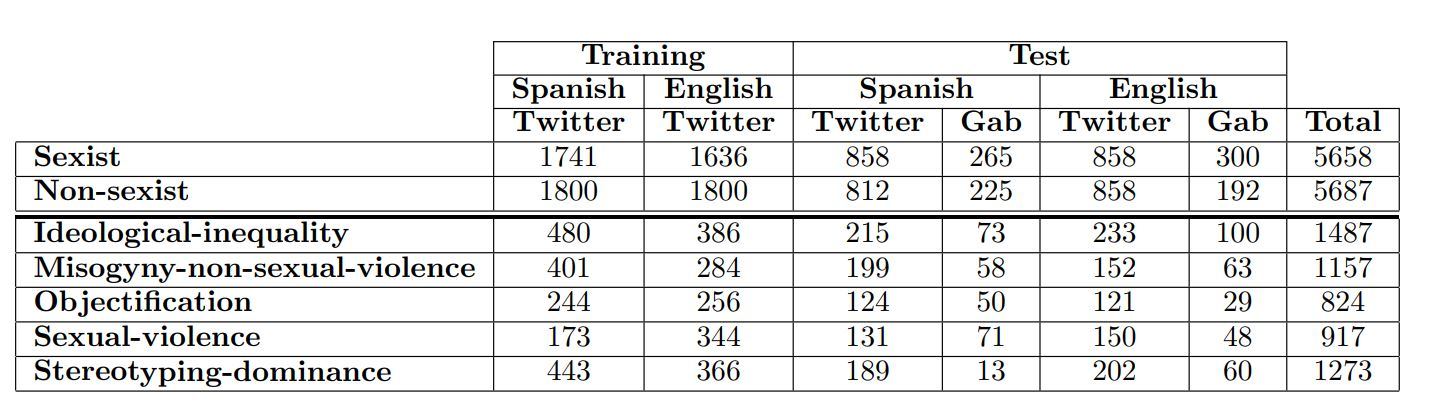
\includegraphics[width=16cm]{imagenes/Arte/dataset_exist2021.jpg}
    \caption{\centering Estadísticas del dataset de EXIST 2021)}
  \label{fig:dataset_exist2021}  
\end{figure}

Respecto a la primera tarea, se puede observar claramente que el dataset está balanceado en los dos idiomas, con 5.658 instancias sexistas y 5.687 instancias no sexistas. Por el otro lado, en la tarea 2, es posible observar algunas diferencias significativas en la distribución de algunas clases como se ejemplifica en la \autoref{fig:dataset_exist2021_task2} generada usando los datos anteriores:

\begin{figure}[H]
    \centering
    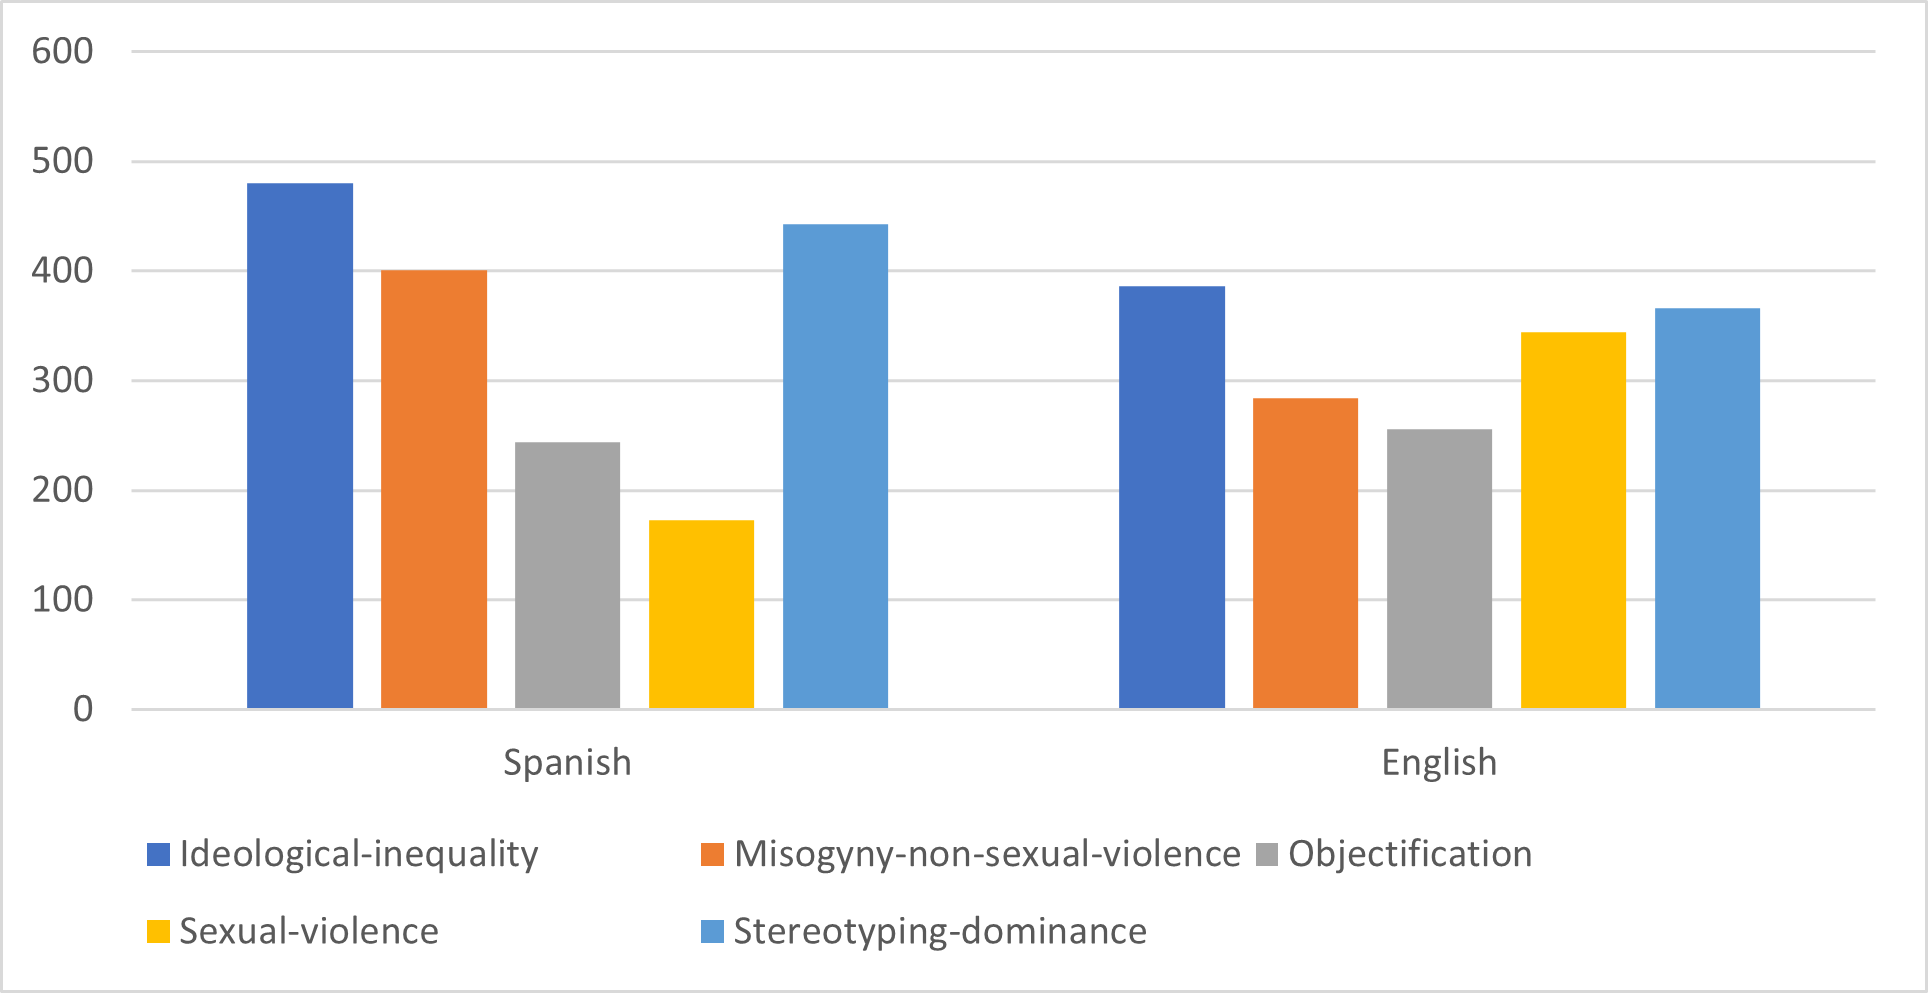
\includegraphics[width=16cm]{imagenes/Arte/task2_exist2021.png}
    \caption{\centering Distribución tarea 2 para EXIST 2021}
    \label{fig:dataset_exist2021_task2}  
\end{figure}

Se puede ver claramente que las diferentes clases están desbalanceadas entre sí. Por un lado, para los textos en español se observa que las clases mayoritarias son la clase de Ideología y desigualdad (480 instancias) y la clase estereotipos y dominancia (443 instancias) donde, por otro lado la clase minoritaria, Violencia-Sexual, posee 173 instancias.

De cara a los tweets en inglés, las instancias bajan para las clases mayoritarias y se equilibran algo más con las demás clases. En este caso la clase mayoritaria, siendo de nuevo Ideología y desigualdad, está compuesta de 386 instancias, lo que respecto de la instancia minoritaria, Objetificación , no supone una diferencia tan alta como para los tweets en español con 256 instancias.

Por otro lado, de cara a la competición en sí, se inscribieron un total de 76 equipos de 11 países diferentes tanto de Europa, Asia y América Del Norte. Sin embargo, solo presentaron modelos 31 equipos para la primera tarea y 27 para la segunda. La mayoría de los participantes se basaron en el uso de Transformers para las dos tareas. Un total de 14 equipos usaron BERT \cite{devlin2018bert} o mBERT (su versión multilingüe) \cite{pires2019multilingual}, 10 usaron una versión española llamada BETO \cite{de2021applying}, 5 RoBERTa \cite{liu2019roberta} y por último 4 equipos usaron una versión multilingüe de RoBERTa llamada XLM-RoBERTa \cite{lample2019cross}.

Además de transformadores algunos equipos usaron Support Vector Machines (SVM) \cite{rameshbhai2019opinion}, Random Forest (RF) \cite{antony2020dynamic}, Long Short Term Memory networks (LSTM) \cite{mostafa2022bidirectional}, Logistic Regresion(LR) \cite{vimal2020application} y con la librería FastText \cite{bhattacharjee2018fasttext}. Sin embargo, como se verá más adelante los modelos basados en Transformers resultaron ser en ambas tareas significativamente mejores.

De cara a los resultados para las diferentes tareas, hay que tener en cuenta que se evalúan desde varias perspectivas teniendo en cuenta el carácter multilingüe de la competición. Por un lado, se ofrecen los resultados para las pruebas realizadas sobre todos los datos (pruebas multilingües), y por otro lado se ofrecen por separado los resultados exclusivamente para los textos en español e inglés como si fueran dos tareas adicionales. Realmente el resultado que importa es el obtenido en la evaluación multilingüe pero los otros dos resultados son interesantes para observar por separado cómo funcionan los modelos planteados específicamente para cada idioma.

Cabe destacar que debido al desbalanceo de datos observado para la tarea 2, la métrica seleccionada para determinar el ganador fue el F1 en lugar del accuracy que fue seleccionado para determinar el ganador en la tarea 1, la cual recordando no se encontraba desbalanceada.

En general para la competición el equipo ganador para ambas tareas fue el equipo AI-UPV\_1. Este equipo utilizó el modelo BERT para los tweets en inglés y BETO para los tweets en español, así como mBERT como modelo multilingüe. Además, también utilizaron modelos de traducción automática para producir nuevos textos sintéticos tanto para inglés como español.

En la primera tarea, el equipo AI-UPV\_1 obtuvo un accuracy de 0.7668 y 0.7944 para inglés y español respectivamente. Así como un accuracy de 0.7804 para el test multilingüe compuesto de tanto los textos en español como en inglés.

Si bien quedó primero, para los resultados en inglés, quedó en tercer lugar por debajo de los equipos SINAI\_TL\_3 y multiaztertest\_1, que obtuvieron 0.7772 y 0.7717 para la tarea 1 en inglés. 

Es interesante mencionar que el equipo SINAI\_TL\_3 usó para la tarea en español BETO, mientras que para clasificar los textos en inglés usaron un modelo basado en la detección de polaridad \cite{sharma2014polarity} (análisis de sentimiento) creado con el dataset InterTASS \cite{martinez2018overview} obteniendo unos resultados de accuracy de 0.7772 y 0.7907 para las tareas de inglés y español respectivamente así como una accuracy global para la tarea 1 de 0.78 quedando en segundo lugar, justo por detrás de AI-UPV\_1.

Para la segunda tarea, el equipo AI-UPV\_1 obtuvo la primera posición para español (F1 de 0.6073), y terceros para inglés (F1 de 0.5507). Obteniendo la primera posición general para la tarea (multilingüe) con un F1 de 0.5787. 

Es interesante mencionar que el equipo que quedó primero en la subtarea en inglés, cuya única referencia accesible es su nombre LHZ\_1, usó un modelo mejorado de BERT y RoBERTa conocido como DeBERTa \cite{he2020deberta}, obteniendo unos resultados de F1 de 0.5604 y 0.5805 para las tareas en inglés y español respectivamente, obteniendo el segundo puesto en la clasificación general con un F1 de 0.5706.

En conclusión, para la competición EXIST 2021 el mejor resultado fue el ofrecido por el equipo AI-PV\_1 para ambas tareas, de 0.7804 de accuracy para la primera y 0.5787 de F1 para la segunda. Estos resultados se obtuvieron usando un sistema basado en varios modelos transformadores basados en BERT diferenciando entre los modelos usados para los textos en inglés y español consiguiendo así maximizar los resultados obtenidos al usar modelos más especializados en cada idioma.

%%%%%%%%%%%%%%%%%%%%%%%%%%%%%%%%%%%%%%%%%%%%%%%%%%%%%
%segunda parte: Exist 2022
%%%%%%%%%%%%%%%%%%%%%%%%%%%%%%%%%%%%%%%%%%%%%%%%%%%%%

Para la segunda entrega de la competición EXIST en 2022 las tareas se mantuvieron iguales, siendo detección del sexismo y clasificación del mismo dentro de las categorías ya mencionadas. De nuevo toda la información de la competición, así como resultados se obtienen directamente del paper relacionado con la misma \cite{rodriguez2022overview}.

Por otro lado, el dataset para esta competición, compuesto de un total de 12.390 instancias, si habría recibido algunos cambios respecto del de 2021. Si bien el dataset se obtenía mayoritariamente del usado para el año anterior, en esta edición se añadió también a la fase del training textos recogidos de la red social GAB \cite{zhou2019elites}, a diferencia de como se hizo en la anterior entrega donde solo se usaban esos textos en la fase de test.

El objetivo de esta modificación era comprobar si afectaría a los resultados de los modelos incluir contenido de una red social sin ningún tipo de control del contenido que se sube a ella durante la fase de entrenamiento.

A continuación se muestra la tabla de distribución de los datos obtenida del paper ya mencionado:

\begin{figure}[H]
    \centering
    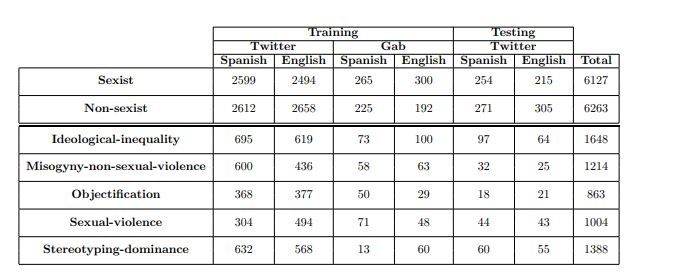
\includegraphics[width=16cm]{imagenes/Arte/dataset_exist2022.jpg}
    \caption{\centering Distribución del dataset para EXIST 2022}
\end{figure}

Si bien para el anterior año se han mostrado también el desbalanceo para la tarea 2, como se puede observar en la tabla ese desbalanceo sigue presente ya que la cantidad de entradas nuevas añadidas al dataset no tenían como objetivo arreglar ese problema y no presentan una proporción lo suficientemente grande del mismo. Es por esto por lo que no se incluye la gráfica al considerarse redundante. 

Al mantener el mismo desbalanceo que la entrega anterior, de cara a las métricas elegidas para determinar los ganadores no hubo cambios y se volvieron a usar accuracy para la tarea 1 y F1 para la tarea 2.

Una característica muy a tener en cuenta es que para esta entrega el set de test fue creado y evaluado por 6 expertos, 3 mujeres y 3 hombres para eliminar cualquier posible sesgo de género, por lo que se considera que la calidad de la anotación es significativamente mejor que la del año anterior.

De nuevo para este año el ganador para las dos tareas es el mismo, en este caso el ganador fue avacaondata\_1. Este equipo presentó para su mejor modelo una idea similar al ganador del año pasado con una unión de modelos, en este caso los modelos eran: BERTweet-large \cite{nguyen-etal-2020-bertweet}, RoBERTa y DeBERTa para los textos en inglés y BETO, BERTIN \cite{de2022bertin}, MarIA-base \cite{gutierrez2021spanish} y ROBERTuito para los textos en español. 

Con esta combinación de modelos obtuvo un accuracy de 0.7996 en la primera tarea bilingüe situándose en una mejora del estado del arte respecto del año pasado de un 0.0192 (2,4\% más). Por otro lado, a diferencia del año anterior este año los resultados en inglés fueron muy superiores con un 0.8422 de accuracy, un 0.065 más que el año anterior (8,36\% más) y para español algo peores que el año pasado con un 0.7801 de accuracy, lo cual lo sitúa 0.0143 por debajo (1,8\% menos). 

Concretamente para la tarea 1, de cara a los textos en español, quedó en 6 puesto obteniendo el ganador de esta subtarea un 0.7801 en accuracy usando una combinación de 10 modelos generados con RoBERTuito y otros 10 modelos generados con BERT usando una semilla diferente en cada entrenamiento de cada uno de los 20 modelos generados.

Es interesante destacar como la tarea en inglés ha mejorado tanto y por el contrario la tarea en español ha incluso empeorado respecto del estado del arte de un año a otro.

Para la segunda tarea, de nuevo ganador, con un 0.5106 de F1 score en los resultados generales lo cual supone una bajada en el estado del arte de 0.0681 (11,7\% menos) aún con una mejora ligera en la precisión del modelo.

Por otro lado, en los resultados específicos obtuvo un F1 de 0.5337 y 0.4867 para inglés y español respectivamente, siendo superado únicamente en los resultados en español por el equipo ELiRF-VRAIN\_3 el cual obtuvo un F1 de 0.4867 usando un de nuevo un sistema de modelos combinado de XLM-RoBERTa, RoBERTa y 3 modelos BERT para los textos en español y XLM-RoBERTa, RoBERTa, BERT, hateBERT \cite{ caselli2020hatebert} y ALBERT \cite{ lan2019albert} para los textos en inglés. 

Es decir, para esta segunda entrega de la competición de EXIST, el ganador y en general los primeros equipos, volvieron a usar un sistema compuesto por varios modelos de Transformer especializados en cada idioma siguiendo la tendencia del año pasado.

En cuanto a los resultados, se han observado mejoras algo bajas para la tarea 1 obteniendo por parte del ganador un accuracy de 0.7996 y peores para la tarea 2, obteniendo por parte del ganador un F1 de 0.5106. Sin embargo, de cara a la tarea 1 la detección de sexismo en inglés ha mejorado significativamente obteniendo un accuracy de 0.8422.

Se plantea una hipótesis acerca de los resultados obtenidos: En primer lugar, la mejora de un año para otro tampoco se puede esperar que sea excesiva y por otro este año, el set de test, solo el set de test que no entrenamiento, ha recibido un análisis mucho más profundo y exhaustivo por parte de 6 expertos. Estas dos razones pueden perfectamente ser la causa de los resultados tan variantes en las diferentes tareas e idiomas de cada una.

En general el estado del arte desde la perspectiva de la detección de sexismo en las redes sociales apunta a que los modelos Transformers pueden obtener resultados muy interesantes, al menos claramente mejores que sus contrapartes ya mencionadas, pero que hay espacio de mejora tanto en los propios modelos como en los datos que se usan para la tarea de entrenamiento. 

Como conclusión se ha observado una clara tendencia por parte de los mejores modelos a usar conocimiento de varios modelos a la vez y no depender exclusivamente de un modelo. Esta es una perspectiva interesante que plantear para futuros trabajos.
\newpage

\chapter{Metodología y Modelos}
\label{cap:modelos}
Este capítulo tiene como objetivo definir las características principales que componen a los diferentes modelos y arquitecturas seleccionadas para el desarrollo de las dos tareas, las cuales surgen como ya se ha mencionado de la competición EXIST 2023. Por un lado, la primera de clasificación binaria de sexismo y la segunda de multiclasificación de la intención de los tweets clasificados como sexistas. Al tratarse de dos tareas similares se usarán para ambas los mismos modelos adaptados para clasificación binaria y clasificación multi clase.

Además, se incluirá un apartado para describir el entorno de trabajo, así como un para describir el preprocesamiento de los textos, fundamental para parte del estudio de este proyecto.

La implementación de las diferentes arquitecturas, así como diferentes procesos realizados durante el estudio se encuentran en el siguiente enlace: \href{https://github.com/ValenUC3M/-NLP-BachelorThesis-GonzaloValenti}{My Bachelor Thesis on NLP}.

Para cada uno de los modelos planteados a continuación el proceso de desarrollo es el mismo. En primer lugar, se definen los hiperparámetros, los cuales quedarán definidos junto a la descripción de cada modelo, así como para cada una de las diferentes versiones del dataset de lo cual se hablará más adelante. 

El entrenamiento se realiza cargando los diferentes modelos seleccionados a través de la librería HuggingFace \cite{HuggingFace}, una vez cargados los modelos, se evalúan las tareas con sus respectivas métricas para cada uno de los datasets de cada tarea.

Adicionalmente cabe destacar que durante este capítulo solo se hablarán tanto de los modelos base como de sus derivaciones a usar durante el trabajo. Esto es importante ya que por ejemplo dentro de la evaluación BERT también se evaluará con la variante multilingüe \cite{bert-base-multilingual-cased} o también por ejemplo roBERTa con una variante conocida como 'twitter-roberta-base-emotion'\cite{twitter-roberta-base-emotion,} de la cual se hablará más adelante.

A continuación se añade una tabla con los hiperparámetros usados para las diferentes pruebas. Cabe destacar que en este trabajo se han priorizado la experimentación de diferentes modelos respecto del ajuste fino de hiperparámetros por lo que, durante la fase de desarrollo, después de algunas pruebas, se llegó a la conclusión de que estos eran los mejores:

\begin{table}[H]
\begin{tabular}{|l|c|c|c|c|}
\hline
\rowcolor[HTML]{9B9B9B} 
{\color[HTML]{000000} \textbf{dataset}}              
& {\color[HTML]{000000} \textbf{batch size}} 
& {\color[HTML]{000000} \textbf{learning rate}} 
& {\color[HTML]{000000} \textbf{epochs}} 
& {\color[HTML]{000000} \textbf{weight decay}} 
\\ \hline
\rowcolor[HTML]{C0C0C0} 
\cellcolor[HTML]{9B9B9B}{\color[HTML]{000000} \textbf{Base}} 
& {\color[HTML]{000000} 16}               
& {\color[HTML]{000000} 2e-5}                  
& {\color[HTML]{000000} 3}             
& {\color[HTML]{000000} 0.01}                  
\\ \hline
\end{tabular}
\caption{Hiperparámetros usados durante la fase de generación de modelos.}
\end{table}


\section{Preprocesado} \label{preprocesado}

Durante el entrenamiento de los modelos se desea plantear dos alternativas para observar las mejorías que ofrece el preprocesamiento en materia de clasificación de tweets. Por un lado, se desea generar los modelos con el texto tal cual viene en el dataset y por el otro lado se desea observar si mejora o no los resultados realizar un preprocesamiento. Para ello primero se debe explicar el proceso que se desea seguir para realizar el preprocesamiento:

El objetivo del preprocesado es limpiar los tweets de toda aquella información que se considere que no aporta información e incluso puede generar ruido a la hora de entrenar. Para ello se ha realizado un breve estudio de preprocesado de tweets y se usa como referencia para ello tanto el estudio de 'tweet-sentiment-analysis-preprocessing' \cite{prepro1} como el trabajo de Abhishek Yadav llamado 'tweets-preprocessing' \cite{prepro2}.

Para realizar el preprocesado principalmente se han utilizado las siguientes librerías:
\begin{itemize}
                \item NLTK \cite{nltk} con el objetivo de eliminar todas las stop words tanto de los tweets en español como los de inglés.
                \item RE \cite{python_re} para generar expresiones regulares capaces de detectar y eliminar aquellas estructuras que se consideren innecesarias.
                \item Emoji \cite{python_emoji} con la cual elimina todos los emoticonos al tratarse de elementos no procesables por parte de los diferentes modelos basados en la arquitectura BERT.
            \end{itemize}


En primer lugar, se realiza un limpiado usando expresiones regulares de las menciones a usuarios al no ofrecer información de la frase y ser más un elemento propio de la red social. Además de las menciones se eliminan todos los hipervínculos, así como los hashtags por la misma lógica que con las menciones. No se desarrolla el proceso de borrado ya que se encuentra explicado de forma completa en el \href{https://github.com/ValenUC3M/-NLP-BachelorThesis-GonzaloValenti}{Github}.

Además del borrado de elementos propios de Twitter, también se eliminan los signos de puntuación, así como caracteres especiales y emojis. Al tratarse de elementos propios del lenguaje como las comas, puntos o paréntesis que no ofrecen realmente información de patrones de cara a los modelos se consideran innecesarios.

Lo último que se procesa de los tweets son las conocidas como 'stop words'. Son aquellas palabras vacías que carecen de significado si se usasen solas y que generalmente no son reconocidas por los diferentes algoritmos de NLP \cite{silva2003importance} ya que su objetivo es el de ofrecer coherencia y un efecto de naturalidad al lenguaje.


\section{Tokenización} \label{tokenización}

Además, los textos deben ser transformados en vectores de números reales para poder ser la entrada de los modelos transformadores que usamos en este trabajo. Este proceso comienza con la tokenización, que consiste en dividir el texto plano en subpartes llamadas tokens. El modelo preentrenado de un transformador proporciona un vector de números reales para cada uno de estos tokens.\cite{venkatesan2022implications}.

BERT utiliza lo que se llama un tokenizador WordPiece \cite{wordpiece}. Funciona dividiendo las palabras en sus formas completas (una palabra se convierte en un token) o en piezas de palabras, donde una palabra puede dividirse en múltiples tokens como se explica más adelante. Gracias a la tokenización se facilita la tarea de NLP al simplificar las palabras y eliminar elementos de ruido consiguiendo mejorar los resultados generales de las tareas \cite{webster1992tokenization}.

El uso de esta técnica permite a BERT representar palabras que no estaban presentes en la colección de textos utilizada para entrenar BERT, ya que generalmente compartirán algunos de los mismos tokens de entrada, que luego se alimentan en las primeras capas de BERT.

Por ejemplo, si cogiéramos la frase 'The embeddings are very useful for NLP' wordpiece generaría el siguiente resultado:

\begin{figure}[H]
    \centering
    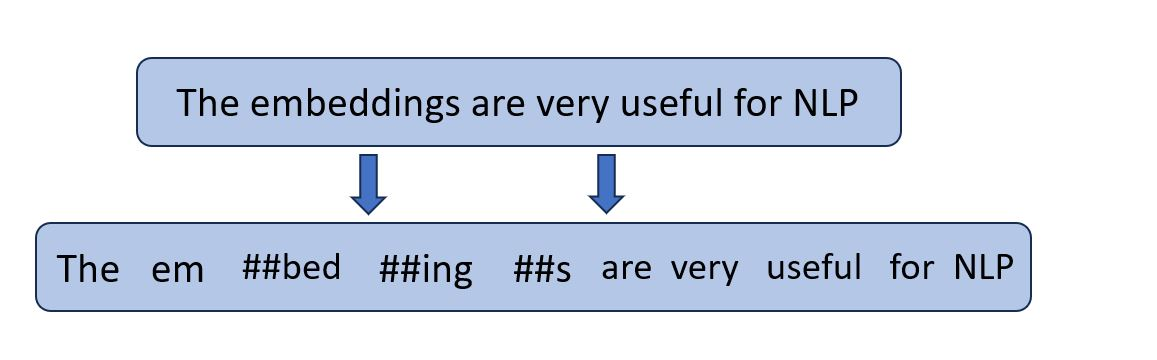
\includegraphics[width=12cm]{imagenes/Modelos/wordpiece.jpg}
    \caption{\centering Ejemplo de uso de Tokenización \cite{Bert-MLM}}
\end{figure}



\section{Modelos}
\subsection{BERT}
BERT o Bidirectional Enconder Representations from Transformers \cite{bert}, se considera el modelo base desde el que derivan los demás modelos de este trabajo. Es por eso que se realizará una explicación extensa sobre el mismo para entender adecuadamente su arquitectura y qué hace exactamente.

El objetivo de BERT \cite{devlin2018bert} es entender el lenguaje, es decir, aprender las diferentes relaciones que existen entre las palabras que componen un lenguaje. Si bien el modelo transformador original \cite{giacaglia2022transformers} estaba compuesto por un codificador y decodificador, BERT únicamente está formado por un codificador que transforma el texto de entrada en un conjunto de vectores (uno por cada token en el texto de entrada). 

En primer lugar, se explica el proceso de preentrenamiento del modelo BERT original. La colección de textos en Ingles usados para su entrenamiento se conoce como Toronto Book corpus \cite{toronto-book-corpus} y está compuesto de alrededor de 11.000 libros sin publicar de todo internet. Sin embargo, este dataset no existe en la actualidad, aunque existen intentos de recrearlo \cite{sgraaf-toronto}.

Para el uso de los Transformer se siguen dos estrategias principales: Por un lado, se realiza un proceso de enmascaramiento (MLM) y por otro lado un sistema de predicción de la siguiente oración (NSP). NSP (Next sentence prediction) es esencialmente un sistema de clasificación binaria que trata de predecir cuándo dos frases aparecen de forma consecutiva o no en un documento \cite{sun-etal-2022-nsp}. MLM (Masked Language Model) se define como un tipo de modelo de lenguaje que requiere ajuste fino para la mayoría de las tareas de procesamiento del lenguaje natural. Los MLMs se evalúan mediante sus puntajes de pseudo-verosimilitud, los cuales se calculan enmascarando tokens uno por uno. \cite{salazar2019masked}. De esta manera se puede predecir el token en cuestión y asignar diferentes pesos y valores a los diferentes tokens en base al entrenamiento realizado.

A continuación, se muestran los parámetros base predefinidos por el modelo sobre los que no se realizarán ajustes, para las diferentes arquitecturas BERT que se usarán durante el estudio de la tarea:

\begin{table}[H]
\begin{center}
\begin{tabular} {|c|c|c|c|c|}
\hline
\rowcolor[HTML]{C0C0C0} 
\textbf{Arquitectura}& \textbf{Capas} & \textbf{Nodos} & \textbf{Attention-Heads} & \textbf{Parámetros} \\ \hline
\cellcolor[HTML]{C0C0C0}\textbf{BERT-Base} & 12 & 768 & 12 & 110M \\ \hline
\cellcolor[HTML]{C0C0C0}\textbf{BERT-Large} & 24 & 1024 & 16 & 340M \\ \hline
\end{tabular}
\end{center}
\label{fig:bert-arch}
\caption{arquitecturas modelos Bert.}
\label{tab:arch-bert}
\end{table}


En primera instancia se debe entender correctamente el proceso de uso de BERT de cara a este trabajo. Una vez que el modelo ha sido preentrenado, y cuenta con una representación vectorial para cada palabra en función de su contexto, el modelo puede ser reentrenado para una tarea concreta ya sea clasificación de textos, análisis de sentimientos, reconocimiento de entidades, etc. A este proceso se le conoce como fine-Tunning. 

Debido a la gran cantidad de entrenamiento requerido y su elevado coste computacional, los modelos que se usan en este proyecto ya han sido preentrenados, y el esfuerzo de este proyecto se centra en el proceso de fine-Tunning. 

El aspecto técnico más innovador de BERT es el uso de aprendizaje bidireccional de Transformers usando mecanismos de atención, lo cual proporciona un contraste significativo respecto de sus anteriores predecesores que procesan de manera unidireccional pudiendo por ello entender el contexto de una palabra usando tanto sus predecesoras como antecesoras. De hecho, como ya se ha comentado, en contraposición con los modelos direccionales, BERT es capaz de leer la secuencia de palabras a la vez. Es por ello que realmente más que un modelo bidireccional, debería ser considerado un modelo no direccional por lo que es capaz de aprender el contexto de una palabra basándose en su entorno \cite{Bert-exp}.

La figura \ref{fig:bert-exp} muestra una descripción de alto nivel de la arquitectura de BERT (que consiste únicamente de un codificador). La entrada es una secuencia de tokens, donde cada palabra es inicializada con un embedding (vector). El codificador, basándose en las dos tareas MLM y NSP, será entrenado para producir una secuencia de embeddings (vectores), donde cada vector representa un token en la secuencia de entrada. 

\begin{figure}[H]
    \centering
    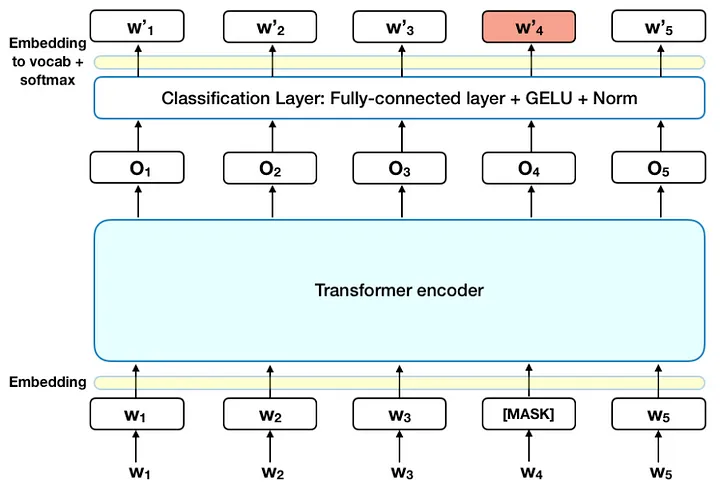
\includegraphics[width=10cm]{imagenes/Modelos/transformer-encoder.png}
    \caption{\centering Arquitectura de alto nivel del sistema transformer-encoder \cite{Bert-exp}}
    \label{fig:bert-exp}
\end{figure}


A continuación, para esta experimentación, se han utilizado dos versiones distintas de BERT: BERT-base-cased y BERT-base-uncased, cuya principal diferencia es que el primero distingue entre mayúsculas y minúsculas, mientras que el segundo no. 

%\section{BERT multilingüe}

BERT también proporciona un modelo multilingüe que fue entrenado con textos de 104 idiomas. Con la versión multilingüe, también experimentamos con las dos versiones: BERT-base-multilingual-cased \cite{bert-base-multilingual-cased} y BERT-base-multilingual-uncased \cite{bert-base-multilingual-uncased}

Sin embargo, durante el entrenamiento, como la mayoría de los textos estaban en inglés en comparación con otros idiomas, como el islandés que es escaso, los idiomas con menos datos fueron sobre muestreados usando técnicas de generación de textos y los idiomas con más datos fueron sub muestreados reduciendo su aparición en el proceso de entrenamiento \cite{pires2019multilingual}.

De cara a su arquitectura Y modelo, cabe aclarar que es la misma usada para bert ya mencionada en la \autoref{tab:arch-bert} mostrada durante la explicación de BERT. Por otro lado, el modelo elegido es el base al tener una limitación en el uso de la memoria para cargar el modelo large.


\subsection{RoBERTa}

Esencialmente RoBERTa es una extensión de BERT desarrollada con el objetivo de corregir algunos de los problemas detectados en BERT por \href{https://ai.facebook.com/research/}{Facebook AI Research (FAIR)}

RoBERTa está basado en BERT, aunque su tokenización es distinta, y está basada en Byte-Pair Encoding a nivel de byte como tokenizador como el que se usaba en GPT-2 \cite{GPT2}. Es decir, su tokenizador se asegura de que las palabras más frecuentes se representen usando un solo token mientras que las menos comunes se separan en tokens más pequeños, lo cual ha demostrado tener buenos rendimientos \cite{galle2019investigating}. 

Por otro lado, RoBERTa modifica el procedimiento de preentrenamiento de BERT entrenando el modelo durante más tiempo (1 Millón de pasos), con lotes más grandes (256 secuencias), sobre más datos (160GB de textos \cite{roberta-intro}) , eliminando el objetivo de predicción de la próxima oración y cambiando dinámicamente el patrón de enmascaramiento aplicado a los datos de entrenamiento, de tal manera que cada secuencia era enmascarada hasta 10 veces de manera diferente garantizando un proceso de aprendizaje más amplio y robusto respecto de BERT \cite{liu2019roberta}.

RoBERTa esencialmente mejora sus resultados respecto a BERT \cite{tarunesh2021trusting} en ciertas tareas considerando a RoBERTa como una versión más optimizada y robusta de BERT \cite{briskilal2022ensemble}. 

A continuación se muestran las variantes de roBERTa usadas:
\begin{enumerate}
    \item RoBERTa-base \cite{roberta-base}: De nuevo compuesta de la misma arquitectura que BERT-base descrita en la \autoref{tab:arch-bert}.
    \item Twitter-RoBERTa-base-emotion \cite{twitter-roberta-base-emotion}: Es una variante de RoBERTa que ha sido ajustada específicamente para el análisis de sentimientos en datos de Twitter. Ha sido entrenado en un conjunto de tweets (alrededor de 58M y está diseñado para identificar la polaridad de los tweets. Si bien a priori se podría considerar que no tiene interés para esta tarea, se ha considerado que al tratarse de una tarea donde se busca identificar el sexismo probablemente un modelo entrenado en sentimientos sea capaz de realizar aproximaciones precisas comparado con quizás la versión base del mismo twitter-roberta-base \cite{twitter-roberta-base}
\end{enumerate}

%\section{Modelo XLM-RoBERTa}
XLM-RoBERTa \cite{xlm-roberta} es una versión multilingüe del modelo RoBERTa, preentrenado en 2,5 TB de datos de CommonCrawl \cite{commoncrawl} que contienen 100 idiomas diferentes. 

Para entender bien XLM-RoBERTa se debe explicar primero el modelo XLM, el cual fue propuesto en el estudio Cross-lingual Language Model Pretraining \cite{lample2019cross} con el objetivo de aprovechar las similitudes y relaciones entre los diferentes idiomas para mejorar su capacidad de generalizar entre ellos.

Si bien XLM-RoBERTa es la versión de tanto XLM como RoBERTa, este no usa los datos de entrenamiento de XLM (como por ejemplo el corpus para francés, español, ruso, árabe y chino conocido como MultiUN \cite{ziemski2016united})  ni de RoBERTa, sino que como ya se ha mencionado usa sus propios datos.

Resumiendo, XLM-RoBERTa es una combinación de dos modelos poderosos: XLM, usando su idea de usar un preentrenamiento multilingüe y RoBERTa, del cual hereda su arquitectura y sistema de preentrenamiento. 

Esto permite que el modelo aprenda una representación bidireccional de la oración y extraiga características útiles desde una perspectiva multilingüe que se pueden utilizar para tareas en datasets multilingües.

A continuación, se muestran los dos modelos basados en XLM-RoBERTa, aunque el segundo modelo no se ha podido utilizar debido a una limitación de memoria en el hardware utilizado para el trabajo:
\begin{enumerate}
    \item XLM-roBERTa-base \cite{xlm-roberta-base}: Como ya se ha comentado posee la misma arquitectura que RoBERTa por lo que también la misma que BERT como se muestra en la \autoref{tab:arch-bert}.
    \item XLM-roBERTa-large \cite{xlm-roberta-large}: Se quería plantear el uso de XLM-Roberta large para ampliar la capacidad del modelo de generalizar y observar si se mejoran los resultados. Sin embargo, la plataforma en la que se realiza el trabajo tiene limitaciones que no cubren con la alta demanda de memoria del modelo ’large’, cuya arquitectura es la misma que para BERT-large mostrada en la \autoref{tab:arch-bert}. Por ello esa aproximación no se realizará y se incluirá en futuras mejoras.
\end{enumerate}


El proceso de estudio será equivalente para todos los modelos generados. Una vez seleccionado un modelo a estudiar se realizará cuatro iteraciones de ejecuciones usando para todas las mismas métricas de entrenamiento (factor de aprendizaje, batch size, épocas etc.) debido a un estudio previo para encontrar las mejores métricas bases para el estudio. 
Cada iteración realizará una de las siguientes combinaciones del dataset base:

\begin{itemize}
    \item Toda la colección de tweets, tanto en español como inglés, sin preprocesar.
    \item La colección de tweets en inglés
    \item Toda la colección de tweets, tanto en español como inglés, preprocesados usando la metodología ya explicada en \autoref{preprocesado}
    \item La colección de tweets en inglés
\end{itemize}

El objetivo de considerar diferentes colecciones para entrenar un modelo es estudiar qué efecto tiene el preprocesado sobre los resultados finales del modelo y, además, conocer qué ocurre si el corpus es entrenado con textos en ambos idiomas. 

\section{Entorno de trabajo}\label{entorno}
Esta sección tiene como objetivo explicar las diferentes herramientas utilizadas durante el desarrollo del trabajo:

    \begin{itemize}
        \item \href{https://colab.research.google.com/}{Google Collaboratory}: Google Collaboratory es una plataforma en línea gratuita que permite a los usuarios escribir y ejecutar código de Python en un entorno colaborativo en la nube. Proporciona acceso a recursos informáticos potentes y escalables, como GPU y TPU, lo que permite a los usuarios trabajar con grandes conjuntos de datos y realizar cálculos complejos de manera más eficiente.
        \item \href{https://code.visualstudio.com/Visual}{Studio Code}: Es un editor de código fuente desarrollado por Microsoft para Windows, Linux y macOS. Es una herramienta muy popular entre los desarrolladores de software, ya que es muy versátil y ofrece una amplia gama de características y extensiones para mejorar la productividad. 
        \item \href{https://www.google.com/intl/es_es/drive/}{Google Drive}: Es un servicio de almacenamiento en la nube gratuito ofrecido por Google que permite a los usuarios almacenar, compartir y sincronizar archivos en línea. También proporciona herramientas de productividad en línea para crear, editar y colaborar en documentos, hojas de cálculo y presentaciones.
        \item \href{https://github.com/}{GitHub}: Es una plataforma de desarrollo colaborativo de software basada en la web que utiliza el control de versiones Git para el seguimiento de cambios en el código fuente. Es una herramienta muy popular entre los desarrolladores de software, ya que permite a los usuarios colaborar en proyectos, contribuir al código y gestionar el flujo de trabajo de desarrollo de software.
        \item \href{https://www.overleaf.com/}{Overleaf}: Overleaf es una herramienta en línea para la edición y colaboración de documentos LaTeX, utilizada principalmente en la creación de documentos científicos y técnicos. Permite a los usuarios trabajar juntos en tiempo real en un solo documento, y proporciona herramientas para la edición, revisión y compilación de documentos LaTeX. En resumen, Overleaf es una herramienta en línea para la edición y colaboración de documentos LaTeX.
        \item \href{https://huggingface.co/}{El ecosistema Hugging Face}: Empezó como un repositorio de modelos Transformers y se ha convertido en un ecosistema para el desarrollo de modelos para NLP donde se pueden encontrar librerías específicas y herramientas para acelerar el uso e investigación en modelos Transformers \cite{tunstall2022natural}. HuggingFace proporciona esencialmente un acceso rápido y versátil a modelos Transformers para todo tipo de tareas y aproximaciones, es por ello que se usará como fuente de modelos durante el desarrollo de este trabajo.

    \end{itemize}
    
Hardware:

    \begin{itemize}
        \item Procesador: AMD Ryzen 5 3600 6-Core Processor 3.59 GHz.
        \item Tarjeta gráfica: Geforce GTX 1660.
        \item RAM: 16,0 GB.
        \item Sistema operativo: Windows 10 Home 64 bits.
    \end{itemize}
    

    
Los detalles del \textbf{Hardware} que ofrece Google Colab son los siguientes:

    \begin{itemize}
        \item Procesador: CPU Intel Xeon 2.20 GHz.
        \item GPU: Tesla K80.
        \item RAM: 13 GB.
        \item Sistema operativo: Linux.
    \end{itemize}
\newpage

\chapter{Evaluación}
Este capítulo del trabajo tiene como objetivo detallar las diferentes partes del proceso de evaluación, desde las métricas, datasets hasta los s resultados obtenidos para los modelos y sus respectivas pruebas.

\section{Métricas} \label{metricas}
Para conocer el desempeño de nuestros modelos de forma cuantitativa es necesario evaluarlos utilizando una serie de métricas. Específicamente en tareas de clasificación como la planteada para este trabajo se consideran las más utilizadas: Accuracy,  precisión, , recall, F1-score en sus versiones macro. \cite{forman2003extensive}.

Para definir estas métricas, es necesario introducir primero los siguientes conceptos: Se entiende como Falso Positivo (en inglés, False Positive FP) como aquella instancia ha sido erróneamente clasificada como positiva por el modelo, pero que en realidad es negativa, Positivo Cierto (en inglés, True Positive, TP) como aquella instancia que es positiva y que ha sido correctamente identificada como positiva por el modelo, Falso Negativo (en inglés, False Negative, FN) como aquella instancia que aun siendo positiva, ha sido incorrectamente clasificada como negativa por el modelo y por último se entiende Cierto Negativo (en inglés, True Negative, TN) como aquella instancia negativa y que ha sido correctamente clasificada como negativa por el modelo.

\subsection{accuracy}
El accuracy mide el porcentaje de acierto de un modelo respecto al número total de instancias \cite{forman2003extensive}.

\begin{equation}
Accuracy = \frac{TP+TN}{Total}
 \label{Accuracy-Formula}
\end{equation}

\subsection{Precisión}
Se define como la proporción de verdaderos positivos con respecto a todas las predicciones positivas, incluidos los falsos positivos y los aciertos. Una baja precisión significa que nuestro modelo de aprendizaje automático produce un gran número de falsos positivos. \cite{forman2003extensive}. 

\begin{equation}
Precision = \frac{TP}{TP+FP}
 \label{Precisión-Formula}
\end{equation}


\subsection{Recall}
Recall, también conocido como tasa de verdaderos positivos (TPR), es el ratio entre el número de aciertos del modelo a la hora de aciertos a la hora de clasificar la clase positiva, y el número total de instancias de la clase positiva (es decir, entre la suma de los falsos negativos y los true positivos). \cite{forman2003extensive}.

Si nuestro modelo produce un bajo recall, significará que el número de falsos negativos (instancias positivas que no son correctamente identificadas) es muy alto. 

\begin{equation}
Recall = \frac{TP}{TP+FN}
 \label{Recall-Formula}
\end{equation}

\subsection{F1-score}
F1-score combina precisión y recall en una sola métrica para tratar de evaluar ambas métricas de manera conjunta, especialmente útil para casos en las que las dos métricas se encuentren muy separadas entre sí. Dado que la puntuación F1 es un promedio de Precisión y Recall, significa que la puntuación F1 (al menos el usado para este proyecto) otorga igual peso a Precisión y Recall \cite{forman2003extensive}. 

\begin{equation}
F1 = 2 * \frac{Precision * Recall}{Precision + Recall}
\label{F1-Score-Formula}
\end{equation}


\subsection{Macro}
Las estadísticas macro \cite{forman2003extensive} evalúan modelos entrenados para problemas de multiclasificación. Se utiliza el promedio macro en caso de desequilibrio de clase (el tamaño de instancias para cada clase es significativamente distinto). Es la media aritmética de las clases individuales relacionadas con la precisión, el recall y la puntuación F1, es decir, es la suma de todos los valores obtenidos por las diferentes clases dividido entre el número total de clases. Se utilizan puntuaciones de promedio macro cuando necesitamos tratar todas las clases por igual para evaluar el rendimiento general del clasificador frente a las etiquetas de clase más comunes.

La media macro del recall es el promedio de todos los puntajes de recall para diferentes clases. El cálculo del promedio macro sería de la siguiente forma:

\begin{equation}
RecallMacroAvg = \frac{Recall_1+Recall_2+...+Recall_n}{num clases}
\label{Recall-Macro-Avg-Formula}
\end{equation}

La media de la precisión macro es el promedio de todos los valores de precisión para las diferentes clases. El cálculo del promedio macro sería de la siguiente forma:

\begin{equation}
PreccMacroAvg = \frac{Prec_1+Prec_2+...+Prec_n}{num clases}
\label{Precision-Macro-Avg-Formula}
\end{equation}

La media de la macro F1 es el promedio de todos los valores de F1 para las diferentes clases. El cálculo del promedio macro sería de la siguiente forma:

\begin{equation}
PreccMacroAvg = \frac{F1_1+F1_2+...+F1_n}{num clases}
\label{F1-Macro-Avg-Formula}
\end{equation}

\section{Dataset} \label{dataset-study}

Durante el trabajo se dispone de una serie de datasets, todos derivados del dataset obtenido de EXIST 2023 \cite{EXIST2023} como ya se mencionó en la introducción. El objetivo fundamental durante ese subapartado será explicar las diferentes variaciones del dataset original, así como estudiar la distribución de datos dentro del mismo.

Exist proporciona un total de 6.920 + 2.076 instancias que se pueden usar para el entrenamiento de los modelos. Adicionalmente proporcionan 1.038 instancias sin clasificar usadas para entregar en la competición con las predicciones generadas, sin embargo, ese dataset no se ha usado al no participar en la competición.

Cabe destacar que de cara a la generación de modelos se planteará una división del dataset final (8896 instancias) en 3 subdatasets (train, validation y test) para seguir un proceso de aprendizaje estándar usando el sistema de validación típico. Además de esto, la subdivisión será de un 80\% de los datos para training, y un 10\% para test y validation, respectivamente. Además, estos subconjuntos se han creado de forma aleatoria, pero garantizando que la distribución de las clases no cambia de un subconjunto a otro. 

En primer lugar, cada tweet fue anotado por 6 anotadores o 'expertos'. De esta forma, cada tweet posee seis distintos veredictos, uno por cada anotador, y también para cada una de las tres subtareas (aunque este trabajo se centre únicamente en las 2 primeras tareas de clasificación binaria y multiclasificación). Es por ello por lo que, por cada tweet y por cada subtarea, hay 6 anotaciones que no son necesariamente iguales.


El formato de cada entrada del dataset es el siguiente:

\begin{enumerate}
        \item id\_EXIST: Id de la entrada.
        \item lang: Idioma del tweet.
        \item tweet: El tweet a procesar.
        \item number\_annotators: Cantidad de anotadores para el tweet (como norma son 6).
        \item annotators: Nombres identificativos para cada uno de los anotadores.
        \item gender\_annotators: Género identificativo para cada uno de los anotadores (como norma 3 mujeres y 3 hombres).
        \item age\_annotators: Franja de edad de cada anotador donde por norma suele haber 2 de cada una de las 3 franjas (18-22, 23-45, 46+).
        \item labels\_task1: Clasificación binaria sobre si es o no sexista realizada por cada anotador.
        \item labels\_task2: Multi Clasificación realizada por cada anotador en base a las clases:
            \begin{itemize}
                \item Reported.
                \item Judgmental.
                \item Direct.
                \item Unknown.
                \item “-” En caso de haber elegido como no sexista en “label\_task1”.
            \end{itemize}
        \item labels\_task3: Asignación de etiquetas por cada anotador, las etiquetas posibles son las siguientes: 
            \begin{itemize}
                \item Objectification.
                \item Sexual-violence.
                \item Stereotyping-Dominance.
                \item Ideological-Inequality.
                \item Mysoginy-Non-Sexual-Violence.
                \item “-” En caso de haber elegido como no sexista en “label\_task1”.
            \end{itemize}
        \item split: Identifica a qué split dentro del dataset pertenece.

\end{enumerate}

Para este trabajo como ya se ha mencionado la tarea número 3, asociada a la 'label\_task3' no se realizará por lo que esa fila de la entrada para todas las entradas del dataset no se tendrá en cuenta y se eliminará del estudio y transformación de los datos.

Además, las categorías annotator, gender y age se eliminan al no aportar información de cara al entrenamiento.


%\subsection{Dataset adaptado}

Para poder trabajar adecuadamente con los datos recibidos es necesario adaptar el dataset que facilite su posterior tratamiento. Se proponen dos variantes con dos objetivos claramente diferenciados: El primer dataset, cuyo objetivo es servir para el análisis de datos, se compondrá de 6 filas por cada entrada del original (una fila por anotador). De esta manera tendremos un dataset con toda la información de distribución de manera clara y precisa. A continuación, se muestra un ejemplo de conversión:

\begin{table}[H]
\begin{tabular}{|
>{\columncolor[HTML]{9B9B9B}}c |
>{\columncolor[HTML]{C0C0C0}}c |
>{\columncolor[HTML]{C0C0C0}}c |
>{\columncolor[HTML]{C0C0C0}}c |
>{\columncolor[HTML]{C0C0C0}}c |
>{\columncolor[HTML]{C0C0C0}}c |
>{\columncolor[HTML]{C0C0C0}}c |}
\hline
{\color[HTML]{000000} \textbf{Annotator}}
& \cellcolor[HTML]{9B9B9B}{\color[HTML]{000000} \textbf{1}} 
& \cellcolor[HTML]{9B9B9B}{\color[HTML]{000000} \textbf{2}}
& \cellcolor[HTML]{9B9B9B}{\color[HTML]{000000} \textbf{3}}
& \cellcolor[HTML]{9B9B9B}\textbf{4} 
& \cellcolor[HTML]{9B9B9B}\textbf{5}
& \cellcolor[HTML]{9B9B9B}\textbf{6} 
\\ \hline
{\color[HTML]{000000} \textbf{Tweet}}    
& {\color[HTML]{000000} tweet}                      
& {\color[HTML]{000000} tweet}                          
& {\color[HTML]{000000} tweet}                           
& tweet                             
& \cellcolor[HTML]{C0C0C0}tweet
& tweet                              
\\ \hline
\textbf{Task 1}                          
& YES                                      
& YES                                                   
& NO                                          
& YES                              
& NO       
& YES                            
\\ \hline
\textbf{Task 2}                          
& DIRECT                                     
& DIRECT                                                   
& \cellcolor[HTML]{C0C0C0}-                        
& DIRECT                        
& -                                 
& \cellcolor[HTML]{C0C0C0}JUDGMENTAL \\ \hline
\end{tabular}
\caption{ejemplo reducción de instancia compuesta por 6 anotadores}
\end{table}

Como se puede observar los 6 anotadores para el mismo tweet clasifican tanto la tarea 1 como la 2 de maneras diferentes entre sí, algunos coincidiendo y otros no. Para facilita el estudio de los datos esa tabla, que representa una instancia teórica del dataset generaría 6 instancias para las cuales se usaría como valor de la celda tweet el mismo valor y para las tareas 1 y 2 sus respectivos valores. 

En segundo lugar, se propone un dataset adaptado donde se reduzca la entrada observada en la tabla anterior a una sola entrada, de tal manera que para los 6 anotadores en lugar de generar 6 instancias se genere una sola. A continuación, se explica y ejemplifica el proceso:

Para las tareas 1 y 2 se cogerá el valor más repetido y en caso de empate se cogerá el que sea más común en el dataset dentro de los valores empatados. Por ejemplo, supongamos que el valor más común para la tarea 1 es 'YES' y para la tarea 2 es 'DIRECT', en caso de tener por ejemplo 2 anotadores que marquen el valor 'DIRECT' y otros dos que marcasen ' JUDGMENTAL', como han empatado a la hora de generar la nueva instancia se seleccionaría 'DIRECT' como su valor. Así como por ejemplo si se tuvieran 4 anotadores con el valor 'YES' para la tarea 1 y 2 con el valor 'NO', se elegiría el valor 'YES' para la instancia reducida.

Se muestra aquí el ejemplo ya planteado en formato tabla:

\begin{table}[H]
\begin{tabular}{|
>{\columncolor[HTML]{9B9B9B}}c |
>{\columncolor[HTML]{C0C0C0}}c |
>{\columncolor[HTML]{C0C0C0}}c |
>{\columncolor[HTML]{C0C0C0}}c |
>{\columncolor[HTML]{C0C0C0}}c |
>{\columncolor[HTML]{C0C0C0}}c |
>{\columncolor[HTML]{C0C0C0}}c |}
\hline
{\color[HTML]{000000} \textbf{Annotator}} & \cellcolor[HTML]{9B9B9B}{\color[HTML]{000000} \textbf{1}} & \cellcolor[HTML]{9B9B9B}{\color[HTML]{000000} \textbf{2}} & \cellcolor[HTML]{9B9B9B}{\color[HTML]{000000} \textbf{3}} & \cellcolor[HTML]{9B9B9B}\textbf{4} & \cellcolor[HTML]{9B9B9B}\textbf{5} & \cellcolor[HTML]{9B9B9B}\textbf{6} \\ \hline
{\color[HTML]{000000} \textbf{Tweet}}    
& {\color[HTML]{000000} tweet}                             
& {\color[HTML]{000000} tweet}                        
& {\color[HTML]{000000} tweet}                             
& tweet                             
& \cellcolor[HTML]{C0C0C0}tweet   
& tweet                             
\\ \hline
\textbf{Task 1}                        
& YES                                                     
& YES                                                     
& NO                                                      
& YES                              
& NO                  
& YES                                
\\ \hline
\textbf{Task 2}                          
& DIRECT                                                   
& DIRECT                                                   
& \cellcolor[HTML]{C0C0C0}-                                 
& JUDGMENTAL                         
& -                   
& \cellcolor[HTML]{C0C0C0}JUDGMENTAL 
\\ \hline
\end{tabular}
\caption{ejemplo reducción de instancia compuesta por 6 anotadores}
\label{not-reduced-data}
\end{table}

La instancia convertida quedaría así:

\begin{table}[H]
\begin{tabular}{|c|c|c|}
\hline
\rowcolor[HTML]{9B9B9B} 
\cellcolor[HTML]{9B9B9B}{\color[HTML]{000000} \textbf{Tweet}} 
& {\color[HTML]{000000} \textbf{Task 1}}
& {\color[HTML]{000000} \textbf{Task 2}} 
\\ \hline
\rowcolor[HTML]{C0C0C0} 
{\color[HTML]{000000} Tweet}                                
& {\color[HTML]{000000} 'YES'}          
& {\color[HTML]{000000} 'DIRECT'}        
\\ \hline
\end{tabular}
\caption{ejemplo reducción de instancia ya reducida}
\label{reduced-data}
\end{table}


%%%%%%%%%%%%%%%%%%%%%EMPIEZA AQUI EL ANÁLISIS DE BALANCES%%%%%%%%%%%%%%%%%%%%%%%
%\subsection{Análisis de datos}
A continuación se va a analizar el dataset desde el punto de vista de la distribución de los datos. En primer lugar, se desea estudiar para la primera tarea si existe alguna clase de desequilibrio en las clases sexista y no sexista dependiendo de la edad o el género.

Se plantea por tanto la siguiente hipótesis: Desde una perspectiva social es probable que exista cierto sesgo en referencia a la identificación del sexismo desde un punto de vista del género o de la edad, para demostrar o corregir esta hipótesis se muestran a continuación los siguientes gráficos:

\begin{figure}[H]
    \centering
    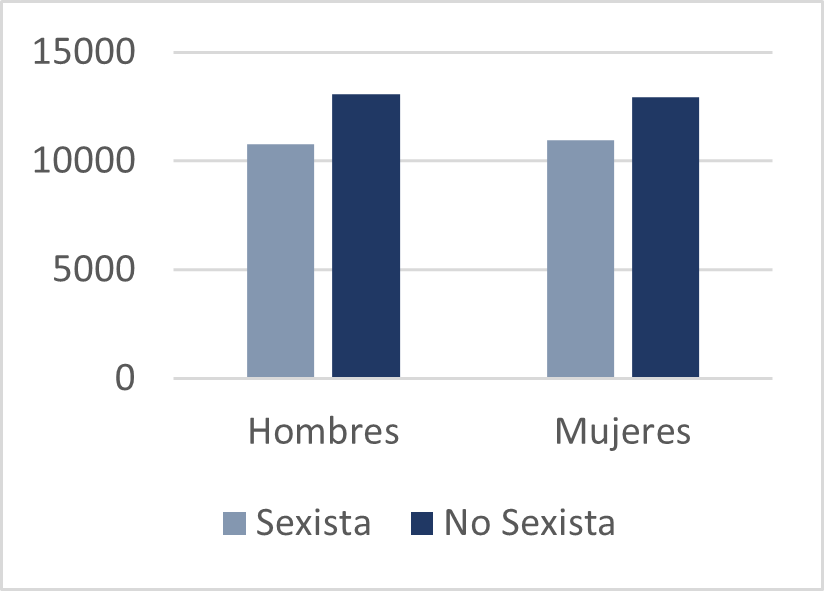
\includegraphics[width=8cm]{imagenes/Evaluacion/dataset_study/gender_task1.png}
    \caption{\centering Distribución de clases para la tarea 1 respecto del género}
    \label{gender-distribution}
\end{figure}

Se puede observar claramente que no existe un sesgo evidente desde una perspectiva del género del anotador con un total de 10.790 y 10.961 de instancias clasificadas como sexistas por hombres y mujeres respectivamente. 

A continuación se muestra la gráfica del balance de clases respecto de la edad para observar si tampoco cumple la hipótesis planteada:

\begin{figure}[H]
    \centering
    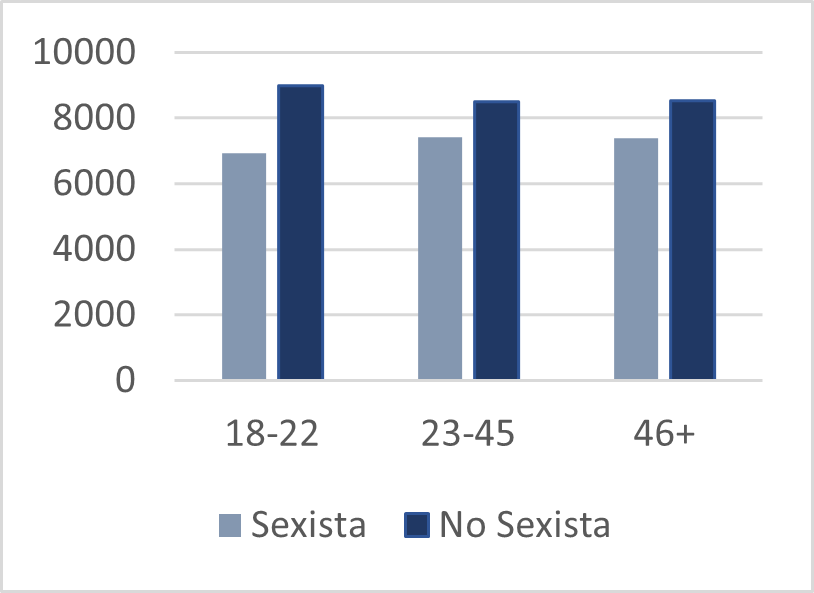
\includegraphics[width=8cm]{imagenes/Evaluacion/dataset_study/age_task1.png}
    \caption{\centering Distribución de clases para la tarea 1 respecto de la edad}
    \label{age-distribution}
\end{figure}

Si bien en este caso se observa una muy ligera tendencia por parte del grupo de edades comprendido entre 18 y 22 años a clasificar más instancias como no, no es lo suficientemente grande como para afirmar que exista un sesgo en base a la edad. Concretamente un total de 8.983 instancias fueron clasificadas como no sexistas respecto de las 8.494 y 8.520 instancias clasificadas como no sexistas por parte de los grupos de edad de 23-45 y 46+ respectivamente.

Por tanto, como se muestra claramente en \autoref{age-distribution} y en \autoref{gender-distribution} el dataset no se encuentra desbalanceado al menos desde una perspectiva de la edad o el género, desmintiendo mi hipótesis inicial.

El siguiente análisis es desde un punto de vista general de la tarea 1 y la tarea 2, como ya se ha mostrado en las tablas \autoref{reduced-data} y \autoref{not-reduced-data} la conversión de las instancias del dataset implica que para cada entrada se simplifica la opinión de 6 anotadores en una media de los mismos para ambas tareas.

Desde un punto de vista analítico esto puede favorecer el desequilibrio de las diferentes clases para cada tarea. Para realizar este análisis vamos a considerar dos datasets, uno en el que se cuenta el valor de cada anotador de forma individual (dataset base) y otro en el que se aplica la reducción ya mencionada y se compacta en una sola instancia la opinión de los 6 anotadores (dataset reducido).

Primero se analiza la distribución de clases para la tarea 1 antes y después de la reducción:

\begin{figure}[H]
    \centering
   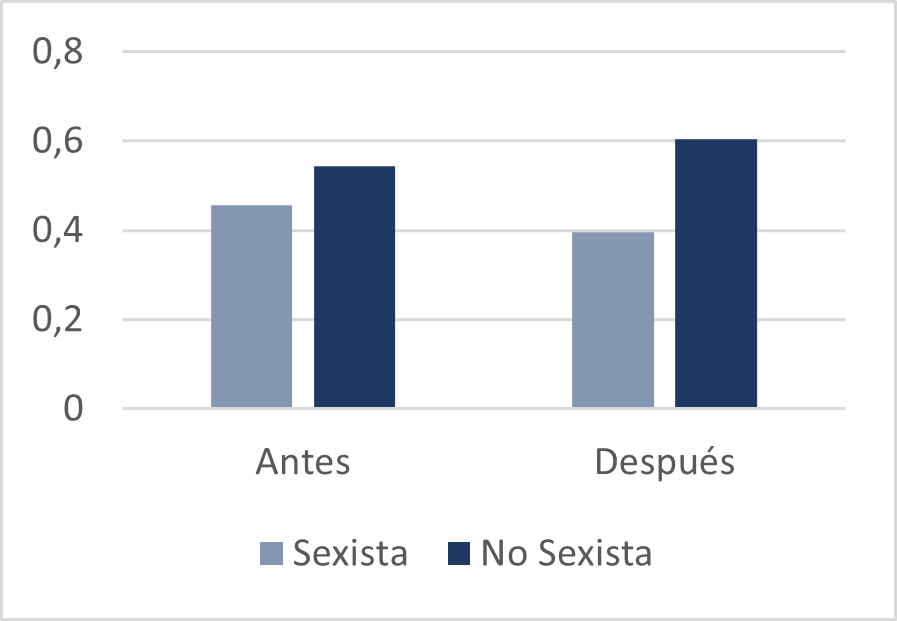
\includegraphics[width=10cm]{imagenes/Evaluacion/dataset_study/task1.png}
    \caption{\centering Distribución de clases antes y después de la reducción del dataset}
    \label{data-distribution-reducing}
\end{figure}

Una vez se realiza la reducción se pasan de tener 6 anotadores a 1 por tweet por lo que los números totales decrecen, es por eso que en lugar de mostrar en el gráfico los valores absolutos para ambas clases se muestran los valores relativos del total en cada dataset, siendo de 47.748 anotaciones respecto de las 7958 obtenidas al reducir (47.748 / 6 = 7958).

Por un lado, antes de la reducción se puede observar que ya existe un ligero desbalance en el dataset con total de 21.751 anotadores que han marcado como sexistas sus tweets respecto de los 25.997 que han marcado como no sexista sus respectivos tweets,  representando los sexistas un 45.55\% del total. Por otro lado, ese desequilibrio se incrementa al realizar la reducción (tiene sentido teniendo en cuenta el algoritmo usado para ello ejemplificado en \autoref{not-reduced-data} y \autoref{reduced-data}, obteniendo un total de 3.152 instancias clasificadas como sexistas frente a las 4.806 instancias clasificadas como no sexistas representando las sexistas un 39.6\% del total.

Es decir, de cara a la evaluación se deberá tener en cuenta el desbalance para la tarea 1 a la hora de analizar las métricas obtenidas para los modelos entrenados.

%Una vez estudiado el balance en la clase 1 se realiza el estudio para la clase 2.

Si bien para la primera tarea se plantea la hipótesis del sesgo de género o edad en base al desequilibrio de los datos, para la tarea 2 no se va a plantear ese mismo análisis. Por otro lado, si se va a estudiar el equilibrio de las diferentes clases que componen la segunda tarea, eliminando todas las instancias que pertenecen a la clase Unknown ya que como se especifica en la descripción de la tarea en \cite{EXIST2023} solo sirven para marcar cuando no se ha podido identificar el subtipo y al tratarse de una clase con solo 82 anotaciones de un total de 21.751 se consideraría ruido.

Además, se debe aclarar que los datos para la tarea 2 solo cuentan con aquellas anotaciones e instancias que hayan sido clasificadas como sexistas en la primera tarea, ya que las que no lo fueron no aportarían información al clasificar la segunda tarea como valor nulo.

De nuevo se va a estudiar el posible desequilibrio de los datos usando un gráfico con los datos antes y después de la reducción como ya se ha explicado anteriormente:

\begin{figure}[H]
    \centering
    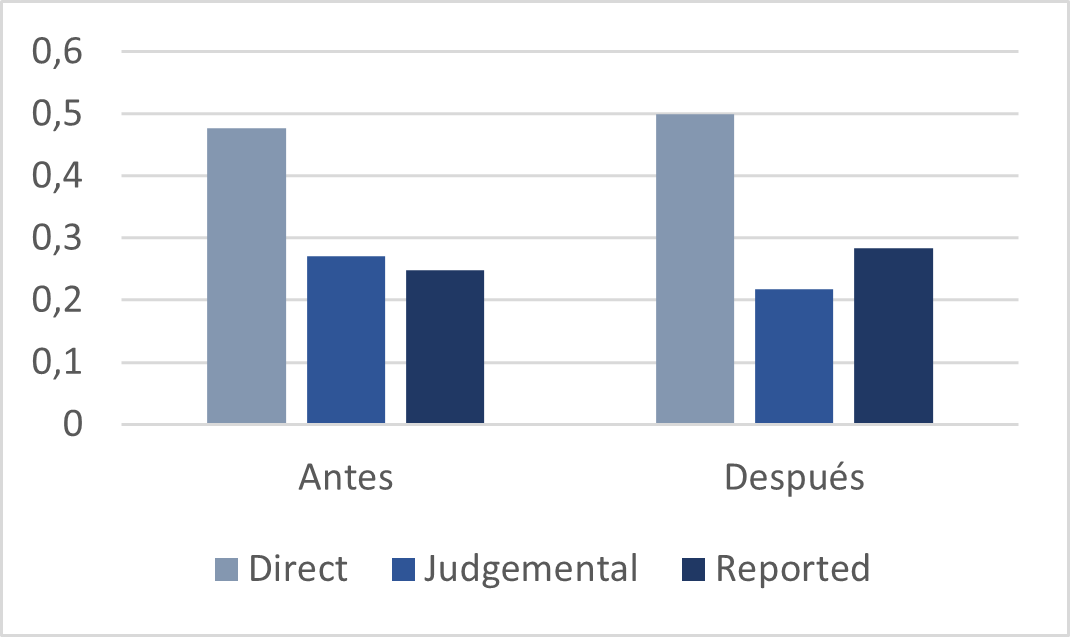
\includegraphics[width=10cm]{imagenes/Evaluacion/dataset_study/task2.png}
    \caption{\centering Balance de clases para la tarea 2 antes y después de la reducción del dataset base}
    \label{balance-task2}
\end{figure}

Por un lado, para los datos antes de la reducción se observa que la clase mayoritaria es claramente la clase Direct con un total de 10.382 anotaciones respecto de las 5.878 y 5.409 anotaciones de las clases Judgemental y Reported respectivamente. Estos resultados representan las siguientes proporciones del total: Un 47,73\% para Direct, un 27,02\% para Judgemental y un 24,86\% para Reported.

Por otro lado, una vez realizada la reducción se observa que la clase mayoritaria sigue siendo la clase Direct con un total de 1575 instancias, seguido de la clase Reported con 892 instancias y Judgemental con 684 instancias. Estos resultados representan las siguientes proporciones del total: Un 49,96\% para Direct, un 21,70\% para Judgemental y un 28,29\% para Reported.

Es decir, antes y después de la reducción la clase Direct compone alrededor del 50\% de los datos, mientras que las otras dos clases componen alrededor del 25\% cada una, sin embargo después de la reducción se ha observado que las clases Judgemental y Reported cambian sus porcentajes pasando Reported de un 24.86\% a un 28.29\% y Judgemental de un 27,02\% a un 21,70\%.

De nuevo habrá que tener en cuenta a la hora de evaluar los resultados obtenidos para los diferentes modelos el desequilibrio entre las diferentes clases para analizar un correcto estudio de los resultados.

%\subsection{Tamaño de tweets}

Además de estudiar la distribución de las clases, se desea estudiar el tamaño de los tweets, considerando como tamaño el número de tokens en el tweet. 

La tabla \ref{tab:lengthtexts} muestra un histograma con la distribución de los tamaños de los tweets. Siendo los valores máximos y mínimos 3 y 78 respectivamente, además de la media de 28,19 tokens. Se puede observar claramente que aproximadamente el 75\% de los tweets se encuentran alrededor de los 40 tokens. 

\begin{figure}[H]
    \centering
    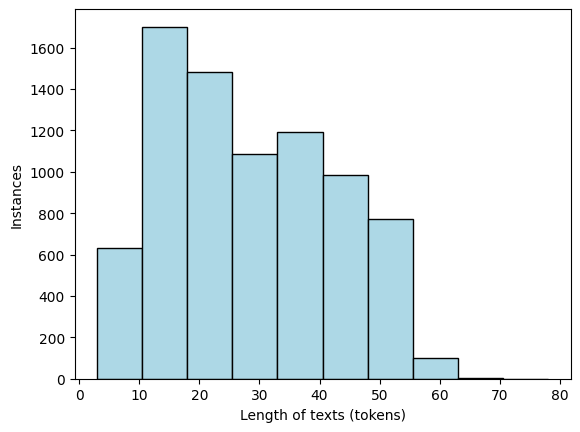
\includegraphics[width=10cm]{imagenes/Evaluacion/dataset_study/lenght_all_tokens.png}
    \caption{\centering Histograma de la longitud de los textos (número de tokens)}
    \label{tab:lengthtexts}
\end{figure}

También se pueden observar unos valores alejados de la media y del centro de gravedad del histograma, pero no se consideran destacables al representar una clara minoría del dataset.

A continuación, se estudia el tamaño de los tweets en base a su clasificación, tanto para la tarea 1 como para la tarea 2. Nuestro objetivo es estudiar si el tamaño de los textos está relacionado con si el tweet es o no sexista, y en el caso de la tarea 2, si está relacionado con el tipo de contenido sexista. Para la tarea 2, la distribución se estudia únicamente sobre el conjunto de tweets clasificados como sexistas como ya se ha comentado anteriormente. 


\begin{figure}[H]
    \centering
    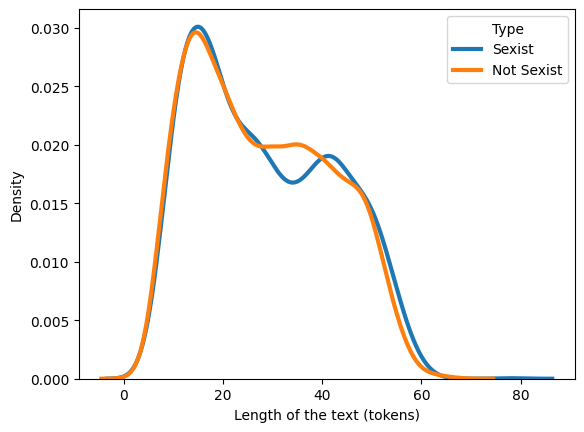
\includegraphics[width=10cm]{imagenes/Evaluacion/dataset_study/sexist_not_sexist_tokens.png}
    \caption{\centering Distribución del tamaño de los tweets (tokens) diferenciando entre tweets sexistas y no sexistas}
    \label{fig:sexist_not_sexist}
\end{figure}

Se puede observar que no existen diferencias destacables en el tamaño de los tweets en relación a si son sexistas o no (Figura \ref{fig:sexist_not_sexist}).

\begin{figure}[H]
    \centering
    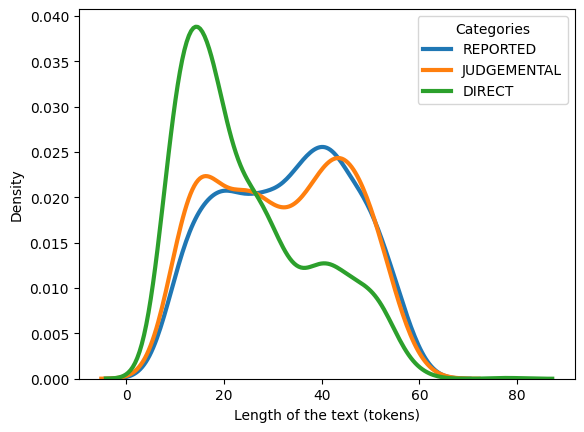
\includegraphics[width=10cm]{imagenes/Evaluacion/dataset_study/task2_lenght_tokens.png}
    \caption{\centering Distribución del tamaño de los tweets (tokens) con contenido sexista en relación a las clases de la tarea 2}
    \label{fig:task2_lenght}

\end{figure}

En la figura \ref{fig:task2_lenght} podemos observar que los tweets clasificados como Direct tienen una tendencia bastante clara a ser más cortos en comparación con los tweets Judgemental y los Reported. Dicho eso, se plantea la siguiente hipótesis: probablemente se debe al carácter inherente de los tweets clasificados como Direct, cuyo objetivo probablemente es simplemente ofender o buscar el agravio sexista, a diferencia de los otros dos que buscan hablar sobre el tema de manera más extendida, aunque esto es solo una hipótesis, y se debería realizar un análisis más detallado sobre los tweets de cada tipo, para poder comprender esta diferencia. 

Para ejemplificar esto se muestran los siguientes tweets, tanto en español como en inglés, donde se puede ver que el tamaño de los tweets Direct es significativamente menor que el de las clases Reported y Judgemental:

\begin{itemize}
    \item Tweet 201073 (Direct): White liberal feminism is a cancer {URL}
    \item Tweet 201075 (Reported): @User1 @User2 No he's just perpetuating the lie that feminism is funded by  Catholic evangelilical sponsors from the US sic. This lie is a direct assault on womens right and ability to self organise. The attack on Catholism is more to do with the Church's history of  rape of its flock.
    \item Tweet 201089 (Judgemental): I laugh at how Celia and her clan pretend to be these great Feminists when in reality they’ve excluded and bullied other women in the house (i.e. Anahi and Alicia)…In celia’s words to Alicia 'I hope that bitch vomits blood' who the fuck even says that unprovoked \#LCDLF
    \item Tweet 100008 (Direct): @User Esta gringa sigue llorando por el gamergate, que 'coincidencia' que tenga pronombres en su perfil
    \item Tweet (Reported): @User1 @User2 @User3 Pues mira no, son hombres, cada uno con su familia, amistades y haciendo vida normal. Igual que los de LaManada, y los que asesinan a diario a sus parejas. Por eso deberíamos preguntarnos qué coño está pasando con los hombres para q actúen así, y qué clase de sociedad queremos.
    \item Tweet (Judgemental): @User1 @User2 @User3 Entonces como así es el mercado lo mejor no es hacer algo para cambiarlo y seguir alimentando el machismo en los consumidores en lugar apoyar a gente como las víctimas del gamergate.Acerca de lo otro, el 'tenían' implica un imperativo entonces no entiendo lo del buscaban.
\end{itemize}



Una vez realizado el preprocesado de los datos siguiendo el esquema planteado en \autoref{preprocesado}, se podrían estudiar de nuevo las diferentes distribuciones dentro del dataset. Sin embargo, se ha observado que las proporciones no varían por lo que solo se va a mostrar el gráfico con el número de tokens al considerar los otros redundantes.

\begin{figure}[H]
    \centering
    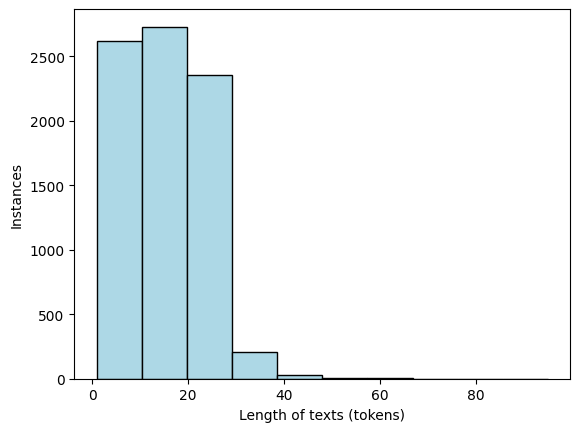
\includegraphics[width=10cm]{imagenes/Evaluacion/dataset_study/preprocessed_text_lenght_tokens.png}
    \caption{\centering Distribución de tamaños en función del número de caracteres preprocesada}
\end{figure}

Lo primero que se puede observar es la bajada en los valores, por un lado sus valores mínimo y máximo se sitúa en 1 y 95 así como su media se sitúa en 15,53 tokens. En segundo lugar, los tweets se han equilibrado alrededor de los valores 9 y 20 a diferencia de \autoref{tab:lengthtexts} cuyos tamaños se encontraban más distribuidos.

\section{Resultados para la tarea de clasificación binaria}
Durante esta sección se van a explicar los diferentes resultados obtenidos para los diferentes modelos planteados en \autoref{cap:modelos}. Realizando de manera adicional un breve análisis sobre aquellos mejores modelos, sus fortalezas, debilidades y posibles razones por las que han obtenido esos resultados.

Tal y como se explicó en el capítulo \ref{cap:modelos}, cada uno de los modelos fue entrenado con distintas versiones del conjunto de entrenamiento: todos los tweets tanto en español como en inglés, ii) únicamente tweets en inglés, iii) todos los tweets preprocesados, y iv) tweets en inglés preprocesados. El objetivo es comparar resultados entre entrenar un modelo utilizando todos los textos disponibles en el dataset (tanto en inglés como en español), y además estudiar el efecto del preprocesado sobre los resultados finales. 

Antes de comenzar es importante destacar el objetivo de este estudio, se desean comparar los modelos para textos en inglés aplicados a una tarea multilingüe respecto de modelos multilingües, para ello se proporcionan resultados tanto solo para los textos en inglés (como referencia) así como para la totalidad de los textos.

\subsection{Bert Base Cased}
El primero de los modelos elegidos es el modelo base de Bert con la variante Cased, la cual recordando, esencialmente trabaja con el dataset original sin quitar todas las mayúsculas. Este modelo suele ser utilizado para tareas como reconocimiento de entidades, donde las mayúsculas y minúsculas si son importantes para discernir si un token o frase son una entidad. Además, es necesario recordar que este modelo fue preentrenado únicamente utilizando textos en inglés. A continuación, se muestran los resultados obtenidos para las cuatro variantes ya mencionadas:

\begin{table}[H]
\begin{tabular}{|c|l|l|l|l|}
\hline
\rowcolor[HTML]{9B9B9B} 
{\color[HTML]{000000} \textbf{Versión}} 
& \multicolumn{1}{c|}{\cellcolor[HTML]{9B9B9B}{\color[HTML]{000000} \textbf{Accuracy}}} 
& \multicolumn{1}{c|}{\cellcolor[HTML]{9B9B9B}{\color[HTML]{000000} \textbf{F1}}} 
& \multicolumn{1}{c|}{\cellcolor[HTML]{9B9B9B}{\color[HTML]{000000} \textbf{Precisión}}} 
& \multicolumn{1}{c|}{\cellcolor[HTML]{9B9B9B}{\color[HTML]{000000} \textbf{Recall}}} 
\\ \hline
\rowcolor[HTML]{E7E6E6} 
\cellcolor[HTML]{9B9B9B}{\color[HTML]{000000} \textbf{Todos los tweets sin preprocesar}}  
& {\color[HTML]{000000} 0.785}  
& {\color[HTML]{000000} 0.775}  
& {\color[HTML]{000000} 0.771}  
& {\color[HTML]{000000} 0.780}                                                     
\\ \hline
\rowcolor[HTML]{E7E6E6} 
\cellcolor[HTML]{9B9B9B}{\color[HTML]{000000} \textbf{Tweets en ingles sin preprocesar}}  
& {\color[HTML]{000000} 0.810} 
& {\color[HTML]{000000} 0.797}                                                 
& {\color[HTML]{000000} 0.794} 
& {\color[HTML]{000000} 0.801}                                                     
\\ \hline
\rowcolor[HTML]{E7E6E6} 
\cellcolor[HTML]{9B9B9B}{\color[HTML]{000000} \textbf{Todos los tweets preprocesados}} 
& {\color[HTML]{000000} 0.765} 
& {\color[HTML]{000000} 0.752}                                                 
& {\color[HTML]{000000} 0.750}                                                    
& {\color[HTML]{000000} 0.756}                                                     
\\ \hline
\rowcolor[HTML]{E7E6E6} 
\cellcolor[HTML]{9B9B9B}{\color[HTML]{000000} \textbf{Tweets en inglés preprocesados}}                                                  
& {\color[HTML]{000000} 0.760}                                                    
& {\color[HTML]{000000} 0.748}                                                 
& {\color[HTML]{000000} 0.744}                                                    
& {\color[HTML]{000000} 0.759}                                                    
\\ \hline
\end{tabular}
\caption{Resultados para Bert-base-cased sobre el conjunto de test.}
\label{bert-base-cased-results}
\end{table}

Se observa una clara tendencia por parte de los modelos no preprocesados a obtener mejores resultados respecto de sus contrapartes con preprocesamiento con unos valores de accuracy 0.785 y 0.810 para los sin preprocesar bilingües e ingleses respectivamente frente a los valores de 0.765 y 0.760 de sus versiones con preprocesado.

En general queda claro que el mejor modelo generado con esta variante es el modelo que solo contiene tweets en inglés lo cual es coherente al tratarse Bert-base de un modelo preentrenado únicamente con textos en inglés. Por tanto, ajustar el modelo para la tarea con también tweets en español no ayuda a mejorar los resultados. 


Además, cabe destacar que, pese a no estar entrenado con textos en castellano, los resultados son bastante buenos respecto de los resultados en inglés, con diferencias muy pequeñas entre los resultados utilizando la colección completa o únicamente utilizando los tweets en inglés. La misma conclusión se obtienen cuando los tweets son preprocesados.

\subsection{Bert Base Uncased}
El segundo de los modelos elegidos es la variación del anterior para el formato uncased donde se ignoraban las mayúsculas y se procesaba todo el texto en minúsculas sin hacer distinción entre palabras iguales con o sin mayúsculas. Posee también un entrenamiento solo en inglés, pero con un uso más genérico y no especializado en entidades como su contraparte.

\begin{table}[H]
\begin{tabular}{|c|l|l|l|l|}
\hline
\rowcolor[HTML]{9B9B9B} 
{\color[HTML]{000000} \textbf{Versión}}  
& \multicolumn{1}{c|}{\cellcolor[HTML]{9B9B9B}{\color[HTML]{000000} \textbf{Accuracy}}} 
& \multicolumn{1}{c|}{\cellcolor[HTML]{9B9B9B}{\color[HTML]{000000} \textbf{F1}}} 
& \multicolumn{1}{c|}{\cellcolor[HTML]{9B9B9B}{\color[HTML]{000000} \textbf{Precision}}} 
& \multicolumn{1}{c|}{\cellcolor[HTML]{9B9B9B}{\color[HTML]{000000} \textbf{Recall}}} 
\\ \hline
\rowcolor[HTML]{E7E6E6} 
\cellcolor[HTML]{9B9B9B}{\color[HTML]{000000} \textbf{Todos los tweets sin preprocesar}}                                                                 
& {\color[HTML]{000000} 0.765}                                                    
& {\color[HTML]{000000} 0.750}                                                 
& {\color[HTML]{000000} 0.749}                                                    
& {\color[HTML]{000000} 0.750}                                                     
\\ \hline
\rowcolor[HTML]{E7E6E6} 
\cellcolor[HTML]{9B9B9B}{\color[HTML]{000000} \textbf{Tweets en ingles sin preprocesar}}                                                  
& {\color[HTML]{000000} 0.741}                                                       
& {\color[HTML]{000000} 0.723}                                                 
& {\color[HTML]{000000} 0.724}                                                        
& {\color[HTML]{000000} 0.721}                                                     
\\ \hline
\rowcolor[HTML]{E7E6E6} 
\cellcolor[HTML]{9B9B9B}{\color[HTML]{000000} \textbf{Todos los tweets preprocesados}}                                                  
& {\color[HTML]{000000} 0.808}                                                   
& {\color[HTML]{000000} 0.800}                                                
& {\color[HTML]{000000} 0.797}                                                    
& {\color[HTML]{000000} 0.819}                                                    
\\ \hline
\rowcolor[HTML]{E7E6E6} 
\cellcolor[HTML]{9B9B9B}{\color[HTML]{000000} \textbf{Tweets en inglés preprocesados}}                                                 
& {\color[HTML]{000000} 0.808}                                                   
& {\color[HTML]{000000} 0.797}                                                 
& {\color[HTML]{000000} 0.792}                                                    
& {\color[HTML]{000000} 0.807}                                                    
\\ \hline
\end{tabular}
\caption{Resultados para Bert-base-uncased sobre el conjunto de test.}
\label{bert-base-uncased-results}
\end{table}


El modelo uncased obtiene mejores resultados que el modelo cased, lo cual es consistente con nuestras conclusiones anteriores. Por tanto, transformar los textos de entrada a minúsculas, permite generalizar mejor y obtener mejores resultados en una tarea de clasificación como esta. En contraposición con los modelos generados para la variante Cased, para Bert uncased se observa que aquellos modelos con preprocesado obtienen resultados significativamente mejores, superándolos con una clara mejora en sus valores de F1 del 5\% para el modelo base y un 7.4\% para el modelo en inglés.

Si bien dentro de los preprocesados, parece que el base obtiene mejores resultados respecto del inglés, cabe destacar un doble factor a tener en cuenta. Por un lado, el dataset para tweets en inglés es significativamente más pequeño por lo que eso puede afectar ligeramente al aprendizaje al tener menor capacidad de generalización y por otro lado las diferencias en resultados no alcanzan ni el 1\% por lo que no se pueden considerar realmente significativas.

\subsection{Bert Base Multilingual}
Los siguientes modelos buscan mejorar los resultados respecto de los modelos de bert-base que contienen tanto los tweets en español como en inglés. Para ello se plantea Bert Base Multilingual usando tanto la variante cased \cite{bert-base-multilingual-cased} como la variante uncased \cite{bert-base-multilingual-uncased} para tener una mayor fuente de datos para analizar. 

En este caso solo se estudian los datasets que contienen todos los tweets ya que no se busca observar las mejoras respecto del inglés, sino las mejoras respecto del total que incluye los tweets en español realizando así el análisis de capacidades multilingües ya mencionado.

\begin{table}[H]
\begin{tabular}{|c|l|l|l|l|}
\hline
\rowcolor[HTML]{9B9B9B} 
{\color[HTML]{000000} \textbf{Versión}} 
& \multicolumn{1}{c|}{\cellcolor[HTML]{9B9B9B}{\color[HTML]{000000} \textbf{Accuracy}}} 
& \multicolumn{1}{c|}{\cellcolor[HTML]{9B9B9B}{\color[HTML]{000000} \textbf{F1}}} 
& \multicolumn{1}{c|}{\cellcolor[HTML]{9B9B9B}{\color[HTML]{000000} \textbf{Precision}}}
& \multicolumn{1}{c|}{\cellcolor[HTML]{9B9B9B}{\color[HTML]{000000} \textbf{Recall}}} 
\\ \hline
\rowcolor[HTML]{E7E6E6} 
\cellcolor[HTML]{9B9B9B}{\color[HTML]{000000} \textbf{Cased}}                           
& {\color[HTML]{000000} 0.767}                                                  
& {\color[HTML]{000000} 0.753}                                      
& {\color[HTML]{000000} 0.752}                                               
& {\color[HTML]{000000} 0.754}                                                     
\\ \hline
\rowcolor[HTML]{E7E6E6} 
\cellcolor[HTML]{9B9B9B}{\color[HTML]{000000} \textbf{Preprocesado Cased}}   
                                               
& {\color[HTML]{000000} 0.772}                                                       
& {\color[HTML]{000000} 0.763}                                                 
& {\color[HTML]{000000} 0.759}                                                        
& {\color[HTML]{000000} 0.770}                                                     
\\ \hline
\rowcolor[HTML]{E7E6E6} 
\cellcolor[HTML]{9B9B9B}{\color[HTML]{000000} \textbf{Uncased}}              
                                                  
& {\color[HTML]{000000} 0.788}                                                       
& {\color[HTML]{000000} 0.774}                                                 
& {\color[HTML]{000000} 0.775}                                                        
& {\color[HTML]{000000} 0.773}                                                     
\\ \hline
\rowcolor[HTML]{E7E6E6} 
\cellcolor[HTML]{9B9B9B}{\color[HTML]{000000} \textbf{Preprocesado Uncased}} 
                                               
& {\color[HTML]{000000} 0.746}                                                      
& {\color[HTML]{000000} 0.730}                                                 
& {\color[HTML]{000000} 0.729}                                                        
& {\color[HTML]{000000} 0.731}                                                     
\\ \hline
\end{tabular}
\caption{Resultados para Bert-base-multilingual sobre el conjunto de test.}
\end{table}

Se observa una caída en los resultados para el dataset preprocesado para el modelo uncased siendo completamente al revés para el modelo cased, algo que ya se había podido observar en \autoref{bert-base-cased-results} y \autoref{bert-base-uncased-results}. Adicionalmente se observa claramente que el mejor modelo es el que no recibe preprocesamiento y se genera usando el modelo Uncased con unos valores F1 de 0.774 y accuracy de 0.788, además de unos valores en las demás métricas muy similares.

Por otro lado, para los dos modelos generados con Cased se observan apenas ninguna diferencia entre ambos (alrededor del 1\%). 

Queda por tanto claro que el mejor modelo generado con la versión multilingüe es creado usando el modelo uncased sin preprocesamiento, pudiendo observar quizás una ligera tendencia por parte de los modelos a obtener mejores resultados cuando no se preprocesa el dataset. Esto se estudiará más adelante.


\subsection{Roberta Base}
El siguiente modelo es Roberta, como ya se ha comentado Roberta es un modelo basado en BERT, que fue entrenado usando grandes colecciones de textos que incluían textos de redes sociales. Por ello se considera que se pueden obtener resultados interesantes en la tarea planteada, aunque sus textos de entrenamiento sean exclusivamente en inglés.

\begin{table}[H]
\begin{tabular}{|c|l|l|l|l|}
\hline
\rowcolor[HTML]{9B9B9B} 
{\color[HTML]{000000} \textbf{Versión}}                                     
& \multicolumn{1}{c|}{\cellcolor[HTML]{9B9B9B}{\color[HTML]{000000} \textbf{Accuracy}}}
& \multicolumn{1}{c|}{\cellcolor[HTML]{9B9B9B}{\color[HTML]{000000} \textbf{F1}}}
& \multicolumn{1}{c|}{\cellcolor[HTML]{9B9B9B}{\color[HTML]{000000} \textbf{Precision}}} 
& \multicolumn{1}{c|}{\cellcolor[HTML]{9B9B9B}{\color[HTML]{000000} \textbf{Recall}}} 
\\ \hline
\rowcolor[HTML]{E7E6E6} 
\cellcolor[HTML]{9B9B9B}{\color[HTML]{000000} \textbf{Todos los tweets sin preprocesar}}                                                             
& {\color[HTML]{000000} 0.783}                                                     
& {\color[HTML]{000000} 0.772}                                               
& {\color[HTML]{000000} 0.770}                                           
& {\color[HTML]{000000} 0.776}                                                  
\\ \hline
\rowcolor[HTML]{E7E6E6} 
\cellcolor[HTML]{9B9B9B}{\color[HTML]{000000} \textbf{Tweets en inglés sin preprocesar}}                                                
& {\color[HTML]{000000} 0.781}                                                     
& {\color[HTML]{000000} 0.777}                                              
& {\color[HTML]{000000} 0.785}                                                   
& {\color[HTML]{000000} 0.809}                                                 
\\ \hline
\rowcolor[HTML]{E7E6E6} 
\cellcolor[HTML]{9B9B9B}{\color[HTML]{000000} \textbf{Todos los tweets preprocesados}}                                                        
& {\color[HTML]{000000} 0.767}                                                     
& {\color[HTML]{000000} 0.740}                                                
& {\color[HTML]{000000} 0.760}                                                  
& {\color[HTML]{000000} 0.731}                                                    
\\ \hline
\rowcolor[HTML]{E7E6E6} 
\cellcolor[HTML]{9B9B9B}{\color[HTML]{000000} \textbf{Tweets en inglés preprocesados}}                                            
& {\color[HTML]{000000} 0.797}                                                    
& {\color[HTML]{000000} 0.785}                                                
& {\color[HTML]{000000} 0.780}                                                      
& {\color[HTML]{000000} 0.793}                                                  
\\ \hline
\end{tabular}
\caption{Resultados para Roberta-base sobre el conjunto de test.}
\label{roberta-base-results}
\end{table}

En estos resultados se puede observar claramente que de nuevo los modelos sin preprocesamiento se comportan mejor que los que si tienen preprocesamiento como ya ha pasado anteriormente. Por un lado, el modelo para los tweets en ingles sin preprocesar obtiene unos valores de F1 de 0.777 y Accuracy de 0.781, y el modelo multilingüe obtiene unos cercanos 0.772 y 0.783 de F1 y Accuracy respectivamente. Sin embargo, sus valores de recall se encuentran algo separados con un 0.775 para el base y un 0.809 para el base en inglés, es decir, el modelo en inglés tiene una mayor capacidad para identificar positivos y no pasarlos por alto como falsos negativos respecto del otro.

Se puede determinar que el mejor modelo para RoBERTa es el modelo base en inglés con unos valores de accuracy y precisión de 0.781 y 0.785 respectivamente lo cual se mantiene coherente al tratarse de un modelo de nuevo creado para tareas en inglés.

\subsection{Twitter RoBERTa base emotion}
El siguiente modelo, Twitter RoBERTa base emotion \cite{twitter-roberta-base-emotion} es una variante de RoBERTa que como ya se ha comentado ha sido ajustada específicamente para el análisis de sentimientos con datos de Twitter. Por ello se considera que puede ofrecer resultados interesantes para nuestra tarea y se ha usado como modelo adicional dentro de Roberta.

\begin{table}[H]
\begin{tabular}{|c|l|l|l|l|}
\hline
\rowcolor[HTML]{9B9B9B} 
{\color[HTML]{000000} \textbf{Versión}}                                    
& \multicolumn{1}{c|}{\cellcolor[HTML]{9B9B9B}{\color[HTML]{000000} \textbf{Accuracy}}}
& \multicolumn{1}{c|}{\cellcolor[HTML]{9B9B9B}{\color[HTML]{000000} \textbf{F1}}}
& \multicolumn{1}{c|}{\cellcolor[HTML]{9B9B9B}{\color[HTML]{000000} \textbf{Precision}}}
& \multicolumn{1}{c|}{\cellcolor[HTML]{9B9B9B}{\color[HTML]{000000} \textbf{Recall}}} 
\\ \hline
\rowcolor[HTML]{E7E6E6} 
\cellcolor[HTML]{9B9B9B}{\color[HTML]{000000} \textbf{Todos los tweets sin preprocesar}}                                                           
& {\color[HTML]{000000} 0.771}                                                     
& {\color[HTML]{000000} 0.754}                                             
& {\color[HTML]{000000} 0.756}                                                    
& {\color[HTML]{000000} 0.752}                                                
\\ \hline
\rowcolor[HTML]{E7E6E6} 
\cellcolor[HTML]{9B9B9B}{\color[HTML]{000000} \textbf{Tweets en inglés sin preprocesar}}                                             
& {\color[HTML]{000000} 0.829}                                                    
& {\color[HTML]{000000} 0.816}                                            
& {\color[HTML]{000000} 0.813}                                                   
& {\color[HTML]{000000} 0.819}                                                   
\\ \hline
\rowcolor[HTML]{E7E6E6} 
\cellcolor[HTML]{9B9B9B}{\color[HTML]{000000} \textbf{Todos los tweets preprocesados}}                                                       
& {\color[HTML]{000000} 0.766}                                                   
& {\color[HTML]{000000} 0.742}                                            
& {\color[HTML]{000000} 0.755}                                                      
& {\color[HTML]{000000} 0.735}                                               
\\ \hline
\rowcolor[HTML]{E7E6E6} 
\cellcolor[HTML]{9B9B9B}{\color[HTML]{000000} \textbf{Tweets en inglés sin preprocesados}}                                           
& {\color[HTML]{000000} 0.784}                                                      
& {\color[HTML]{000000} 0.762}                                                
& {\color[HTML]{000000} 0.766}                                                     
& {\color[HTML]{000000} 0.759}                                                     
\\ \hline
\end{tabular}
\caption{Resultados para Twitter-RoBERTa-base-emotion sobre el conjunto de test.}
\end{table}

Lo primero que se puede observar de manera clara y directa es que los resultados el modelo base en inglés son los mejores hasta el momento con unos valores de 0.829 y 0.816 de Accuracy y F1 respectivamente. Teniendo en cuenta que este modelo se ha entrenado con una base de datos de tweets en inglés tiene bastante sentido observar estos resultados.

Por otro lado, las métricas para el modelo base no son para nada malas, de hecho, se sitúan en la parte superior en calidad respecto del resto de modelos ya estudiados. Es interesante ver como modelos preentrenados con tweets son capaces claramente de adaptarse y trabajar con mayor facilidad con el dataset.

Además, de nuevo se vuelve a observar como aquellos modelos que no poseen preentrenamiento sobre los datos obtienen mejores resultados respecto de aquellos que sí.

\subsection{XLM-Roberta-base}
XLM-Roberta \cite{xlm-roberta} es el equivalente multilingüe de RoBERTa, ofreciendo en la teoría una capacidad de generar modelos con varios lenguajes a la vez, superior a la que ofrecía RoBERTa como ya se había comentado. El objetivo es observar si existen mejoras respecto de su contraparte para alguna de las 4 versiones generadas y en caso de existir considerarlas para la solución final.

Una característica reseñable de XLM es su entrenamiento, como ya se mencionó en apartados anteriores, basado en aproximadamente textos de 100 lenguajes diferentes, siendo el inglés y el castellano los idiomas con mayor número de textos.

\begin{table}[H]
\begin{tabular}{|c|l|l|l|l|}
\hline
\rowcolor[HTML]{9B9B9B} 
{\color[HTML]{000000} \textbf{Versión}}                                    
& \multicolumn{1}{c|}{\cellcolor[HTML]{9B9B9B}{\color[HTML]{000000} \textbf{Accuracy}}} 
& \multicolumn{1}{c|}{\cellcolor[HTML]{9B9B9B}{\color[HTML]{000000} \textbf{F1}}}
& \multicolumn{1}{c|}{\cellcolor[HTML]{9B9B9B}{\color[HTML]{000000} \textbf{Precision}}} 
& \multicolumn{1}{c|}{\cellcolor[HTML]{9B9B9B}{\color[HTML]{000000} \textbf{Recall}}} 
\\ \hline
\rowcolor[HTML]{E7E6E6} 
\cellcolor[HTML]{9B9B9B}{\color[HTML]{000000} \textbf{Todos los tweets sin preprocesar}}                                              
& {\color[HTML]{000000} 0.782}                                                    
& {\color[HTML]{000000} 0.775}                                             
& {\color[HTML]{000000} 0.772}                                   
& {\color[HTML]{000000} 0.786}                                                
\\ \hline
\rowcolor[HTML]{E7E6E6} 
\cellcolor[HTML]{9B9B9B}{\color[HTML]{000000} \textbf{Tweets en inglés sin preprocesar}}                                      
& {\color[HTML]{000000} 0.765}                                                      
& {\color[HTML]{000000} 0.751}                             
& {\color[HTML]{000000} 0.747}                            
& {\color[HTML]{000000} 0.759}                                         
\\ \hline
\rowcolor[HTML]{E7E6E6} 
\cellcolor[HTML]{9B9B9B}{\color[HTML]{000000} \textbf{Todos los tweets preprocesados}}                                    
& {\color[HTML]{000000} 0.736}                                                     
& {\color[HTML]{000000} 0.724}            
& {\color[HTML]{000000} 0.721}                                                   
& {\color[HTML]{000000} 0.729}                                                 
\\ \hline
\rowcolor[HTML]{E7E6E6} 
\cellcolor[HTML]{9B9B9B}{\color[HTML]{000000} \textbf{Tweets en inglés preprocesados}} 

& {\color[HTML]{000000} 0.757}                                                                                            
& {\color[HTML]{000000} 0.744}                                   
& {\color[HTML]{000000} 0.740}                                         
& {\color[HTML]{000000} 0.753}                                   
\\ \hline
\end{tabular}
\caption{Resultados para XLM-RoBERTa-base sobre el conjunto de test.}
\end{table}

En general los resultados obtenidos son peores en todos los aspectos respecto de los resultados de RoBERTa mostrados en la \autoref{roberta-base-results}. Concretamente el único que obtiene resultados similares es el modelo creado con todos los tweets sin preprocesar con unos valores de F1 y Accuracy de 0.754 y 0.771 respectivamente. 

Eso sí, de igual manera que para los demás modelos se observa que aquellos modelos generados con los datos preprocesados obtienen peores valores respecto de aquellos que no han recibido preprocesamiento.

\subsection{Mejores modelos}

Durante este apartado se van a comparar directamente los mejores modelos encontrados durante las diferentes pruebas realizadas para la tarea de clasificación binaria. Los modelos se han obtenidos de los ya analizados y por ende este apartado solo tiene como objetivo determinar de manera clara y analítica cuales son los 2 mejores modelos finales para su análisis. 

Cabe destacar que se realizará una subdivisión final en la que, de esos dos modelos, uno se elegirá entre los modelos bilingües y otro se elegirá de los modelos únicamente ingleses. De esta manera se tendrá una perspectiva clara sobre las capacidades de los modelos presentados basados en bert para trabajar con idiomas diferentes del inglés.

A continuación, se muestran los mejores modelos solo con tweets en inglés:

\begin{table}[H]
\begin{tabular}{|l|l|l|l|l|}
\hline
\rowcolor[HTML]{9B9B9B} 
\multicolumn{1}{|c|}{\cellcolor[HTML]{9B9B9B}{\color[HTML]{000000} \textbf{Versión}}}      
& \multicolumn{1}{c|}{\cellcolor[HTML]{9B9B9B}{\color[HTML]{000000} \textbf{Accuracy}}}
& \multicolumn{1}{c|}{\cellcolor[HTML]{9B9B9B}{\color[HTML]{000000} \textbf{F1}}} 
& \multicolumn{1}{c|}{\cellcolor[HTML]{9B9B9B}{\color[HTML]{000000} \textbf{Precision}}}
& \multicolumn{1}{c|}{\cellcolor[HTML]{9B9B9B}{\color[HTML]{000000} \textbf{Recall}}} 
\\ \hline
\rowcolor[HTML]{E7E6E6} 
\cellcolor[HTML]{9B9B9B}{\color[HTML]{000000} \textbf{Bert-base-cased inglés}}                                                           
& {\color[HTML]{000000} 0.8106}                                                
& {\color[HTML]{000000} 0.7973}                                             
& {\color[HTML]{000000} 0.7940}                                 
& {\color[HTML]{000000} 0.8018}                                                 
\\ \hline
\rowcolor[HTML]{E7E6E6} 
\cellcolor[HTML]{9B9B9B}{\color[HTML]{000000} \textbf{Bert-base-uncased Inglés}}                                                       
& {\color[HTML]{000000} 0.808}                                              
& {\color[HTML]{000000} 0.800}                                                
& {\color[HTML]{000000} 0.797}                                                    
& {\color[HTML]{000000} 0.819}                                                   
\\ \hline
\rowcolor[HTML]{E7E6E6} 
\cellcolor[HTML]{9B9B9B}{\color[HTML]{000000} \textbf{Roberta-base inglés}}                                                            
& {\color[HTML]{000000} 0.781}                                               
& {\color[HTML]{000000} 0.777}                                           
& {\color[HTML]{000000} 0.785}                                            
& {\color[HTML]{000000} 0.809}                                                   
\\ \hline
\rowcolor[HTML]{E7E6E6} 
\cellcolor[HTML]{9B9B9B}{\color[HTML]{000000} \textbf{Twitter-roberta-base-emotion inglés}}                                            
& {\color[HTML]{000000} 0.821}                                                       
& {\color[HTML]{000000} 0.809}                                              
& {\color[HTML]{000000} 0.805}                                                      
& {\color[HTML]{000000} 0.816}                                                   
\\ \hline
\end{tabular}
\caption{Mejores modelos primera tarea solo tweets en inglés.}
\end{table}

En general, podemos observar que los modelos se encuentran alrededor del 80\% de media para las diferentes métricas estudiadas. Esto se cumple salvo para un modelo, el mejor de ellos de hecho, el modelo basado en Roberta y twitter 'Twitter-roberta-base-emotion'. Este modelo de todos los planteados era de manera teórica el más consistente con el dataset de este trabajo y por ende era esperable que fuera el que mejor resultados obtuviera al menos de cara a los tweets en inglés. Concretamente ha obtenido unos valores de 0.821 y 0.809 para Accuracy y F1 respectivamente.

A continuación, se muestran sus diferentes métricas desglosadas en un formato donde poder analizar de manera más precisa sus resultados, mostrando los valores obtenidos tanto de forma general como para cada label de manera específica, así como la media ponderada de las mismas:

\begin{table}[H]
\begin{tabular}{|
>{\columncolor[HTML]{9B9B9B}}l |
>{\columncolor[HTML]{E7E6E6}}l |
>{\columncolor[HTML]{E7E6E6}}l |
>{\columncolor[HTML]{E7E6E6}}l |}
\hline
\multicolumn{1}{|c|}{\cellcolor[HTML]{9B9B9B}{\color[HTML]{000000} \textbf{Versión}}}
& \multicolumn{1}{c|}{\cellcolor[HTML]{9B9B9B}{\color[HTML]{000000} \textbf{F1}}} 
& \multicolumn{1}{c|}{\cellcolor[HTML]{9B9B9B}{\color[HTML]{000000} \textbf{Precision}}} 
& \multicolumn{1}{c|}{\cellcolor[HTML]{9B9B9B}{\color[HTML]{000000} \textbf{Recall}}}
\\ \hline
{\color[HTML]{000000} \textbf{No Sexista}}                                 
& {\color[HTML]{000000} 0.85}                                                
& {\color[HTML]{000000} 0.88}                                                            
& {\color[HTML]{000000} 0.81}                                                         
\\ \hline
{\color[HTML]{000000} \textbf{Sexista}}                                           
& {\color[HTML]{000000} 0.75}                                                 
& {\color[HTML]{000000} 0.71}                                                        
& {\color[HTML]{000000} 0.81}                                                         
\\ \hline
{\color[HTML]{000000} \textbf{Weighted Average}}                                   
& {\color[HTML]{000000} 0.81}                                                    
& {\color[HTML]{000000} 0.82}                                                     
& {\color[HTML]{000000} 0.81}                                                    
\\ \hline
\end{tabular}
\caption{Métricas desglosadas Twitter-roberta-base-emotion.}
\end{table}

Antes de comenzar es importante mencionar el uso de medias ponderadas para las métricas desglosadas con el objetivo de tener una visión en conjunto de los resultados desde un punto de vista relativo y no absoluto.

Los resultados del conjunto de pruebas indican que el modelo tiene un rendimiento bastante bueno para la tarea de clasificación binaria, con una puntuación de F1 de 0.75 para sexista y 0.85 para No Sexista. Además, la precisión es razonablemente alta para ambos casos, con una precisión de 0.71 para sexista y 0.88 para No Sexista. El recall también es bastante bueno para ambos casos, con un recall de 0.78 para sexista y 0.76 para No Sexista.

Se puede observar una ligera tendencia hacia clasificar el 'no' correctamente, esto se puede deber al tratarse de la clase mayoritaria en el dataset. De no tenerse en cuenta esto podría llevar a mayores errores en el futuro como sobre entrenamiento, pero de cara a estas pruebas no se considera una tara lo suficientemente grande como para considerarla un problema.

Por último, para comprobar la teoría planteada se va a estudiar brevemente la matriz de confusión generada usando YES para sexista y NO para No Sexista:

\begin{figure}[H]
    \centering
    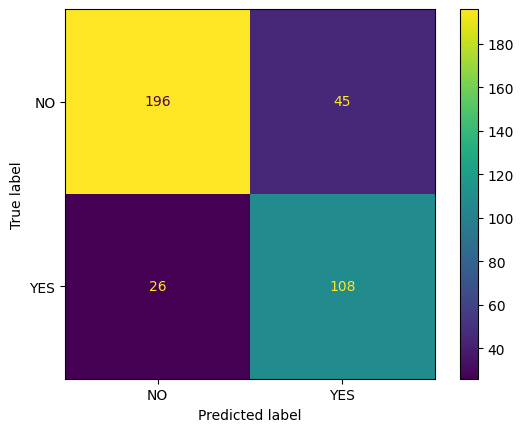
\includegraphics[width=10cm]{imagenes/Evaluacion/confusion_matrix/twitter_roberta_base_emotion-english-dirty.png}
    \caption{\centering matriz de confusión para TWITTER-ROBERTA-BASE-EMOTION}
\end{figure}


Se puede observar inmediatamente que se han clasificado correctamente 196 instancias de la etiqueta No Sexista, así como 108 de Sexista. Por el otro lado, para Sexista se observan un total de 26 instancias mal clasificadas respecto del total de 134 (un 19\%) y para No Sexista se observan 45 instancias mal clasificadas de un total de 241 (un 19\%) pudiendo determinar que si bien en las métricas se observan ciertas tendencias al No Sexista como ya se teorizaba, en la matriz de confusión no se observan evidencias de ello. En conclusión, tras analizar la matriz de confusión, así como las diferentes métricas se obtiene para este modelo un accuracy del 81.06\%.

Por el otro lado tenemos los mejores modelos para la tarea en su formato bilingüe:

\begin{table}[H]
\begin{tabular}{|l|l|l|l|l|}
\hline
\rowcolor[HTML]{9B9B9B} 
\multicolumn{1}{|c|}{\cellcolor[HTML]{9B9B9B}{\color[HTML]{000000} \textbf{Versión}}} 
& \multicolumn{1}{c|}{\cellcolor[HTML]{9B9B9B}{\color[HTML]{000000} \textbf{Accuracy}}} 
& \multicolumn{1}{c|}{\cellcolor[HTML]{9B9B9B}{\color[HTML]{000000} \textbf{F1}}} 
& \multicolumn{1}{c|}{\cellcolor[HTML]{9B9B9B}{\color[HTML]{000000} \textbf{Precision}}} 
& \multicolumn{1}{c|}{\cellcolor[HTML]{9B9B9B}{\color[HTML]{000000} \textbf{Recall}}} 
\\ \hline
\rowcolor[HTML]{E7E6E6} 
\cellcolor[HTML]{9B9B9B}{\color[HTML]{000000} \textbf{Bert-base-cased}}                                                              
& {\color[HTML]{000000} 0.785}                                                     
& {\color[HTML]{000000} 0.775}                                                 
& {\color[HTML]{000000} 0.771}                                                       
& {\color[HTML]{000000} 0.780}                                                   
\\ \hline
\rowcolor[HTML]{E7E6E6} 
\cellcolor[HTML]{9B9B9B}{\color[HTML]{000000} \textbf{Bert-base-multilingual-uncased}}                                                  
& {\color[HTML]{000000} 0.788}                                                    
& {\color[HTML]{000000} 0.774}                                                
& {\color[HTML]{000000} 0.775}                                                          
& {\color[HTML]{000000} 0.773}                                                   
\\ \hline
\rowcolor[HTML]{E7E6E6} 
\cellcolor[HTML]{9B9B9B}{\color[HTML]{000000} \textbf{Twitter-roberta-base-emotion}}                                               
& {\color[HTML]{000000} 0.771}                                        
& {\color[HTML]{000000} 0.754}                                               
& {\color[HTML]{000000} 0.756}                         
& {\color[HTML]{000000} 0.752}                                         
\\ \hline
\rowcolor[HTML]{E7E6E6} 
\cellcolor[HTML]{9B9B9B}{\color[HTML]{000000} \textbf{XLM-roBERTa}}                                       
& {\color[HTML]{000000} 0.782}                                              
& {\color[HTML]{000000} 0.775}                                            
& {\color[HTML]{000000} 0.772}                                                
& {\color[HTML]{000000} 0.786}                                                 
\\ \hline
\end{tabular}
\caption{Mejores modelos primera tarea bilingüe.}
\end{table}

Para estos resultados observamos unos números muy similares entre los modelos salvo para el modelo generado con twitter-roberta-base-emotion que se obtienen peores resultados, todos los demás rondando el 78\% en todas las métricas. Es decir, se sitúan algo por debajo de los mejores en inglés como era de esperar. 

Si hubiera que elegir un mejor modelo, aunque no sea por mucho el mejor modelo es el generado por Bert multilingüe uncased, probablemente debido a su arquitectura y su capacidad de generalizar en varios idiomas es lo que le permite obtener unos mejores resultados, aunque estos no sean significativamente mejores que los demás modelos.

A continuación, se muestran sus diferentes métricas desglosadas en un formato donde poder analizar de manera más precisa sus resultados, mostrando los valores obtenidos tanto de forma general como para cada label de manera específica, así como la media ponderada de las mismas:

\begin{table}[H]
\begin{tabular}{|
>{\columncolor[HTML]{9B9B9B}}l |
>{\columncolor[HTML]{E7E6E6}}l |
>{\columncolor[HTML]{E7E6E6}}l |
>{\columncolor[HTML]{E7E6E6}}l |}
\hline
\multicolumn{1}{|c|}{\cellcolor[HTML]{9B9B9B}{\color[HTML]{000000} \textbf{Versión}}} 
& \multicolumn{1}{c|}{\cellcolor[HTML]{9B9B9B}{\color[HTML]{000000} \textbf{F1}}} 
& \multicolumn{1}{c|}{\cellcolor[HTML]{9B9B9B}{\color[HTML]{000000} \textbf{Precision}}} 
& \multicolumn{1}{c|}{\cellcolor[HTML]{9B9B9B}{\color[HTML]{000000} \textbf{Recall}}} 
\\ \hline
{\color[HTML]{000000} \textbf{No Sexista}}                                              
& {\color[HTML]{000000} 0.82}                                                    
& {\color[HTML]{000000} 0.79}                                                        
& {\color[HTML]{000000} 0.85}                                                        
\\ \hline
{\color[HTML]{000000} \textbf{Sexista}}                                             
& {\color[HTML]{000000} 0.71}                                                    
&{\color[HTML]{000000} 0.75}                                                    
& {\color[HTML]{000000} 0.68}                                               
\\ \hline
{\color[HTML]{000000} \textbf{Weighted Average}}                                  
& {\color[HTML]{000000} 0.78}                                              
& {\color[HTML]{000000} 0.78}                                                  
& {\color[HTML]{000000} 0.78}                                                         
\\ \hline
\end{tabular}
\caption{Métricas Bert-multilingual-uncased.}
\end{table}

Se puede ver claramente en la tabla como el modelo tiende a clasificar mejor los textos no sexistas respecto de los sexistas con unos valores de F1 de 0.82 y 0.71 respectivamente. También es interesante destacar como la clase Sexista tiene un recall muy bajo de 0.68 por lo que se asume que tiene una alta tendencia a clasificar falsos sexistas.

En resumen, el modelo tiene una clara tendencia a clasificar mejor los tweets no sexistas que los sexistas, esto tiene sentido recordando las proporciones del dataset y el posible mayor aprendizaje para detectar no sexistas. Esto además se puede observar aún mejor con el valor de recall de 0.85.

Por último, para comprobar las conclusiones planteadas, se va a estudiar brevemente la matriz de confusión generada del conjunto de test:

\begin{figure}[H]
    \centering
    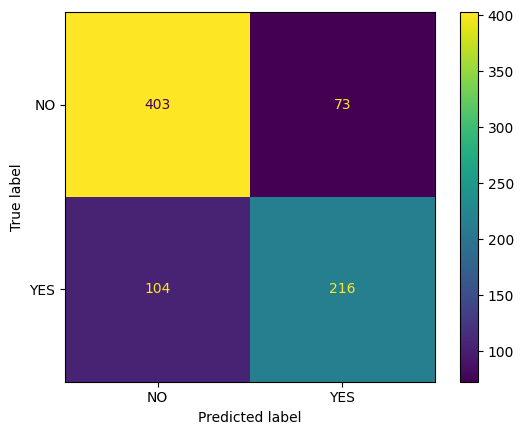
\includegraphics[width=10cm]{imagenes/Evaluacion/confusion_matrix/bert_base_multilingual-uncased-all-dirty.png}
    \caption{\centering matriz de confusión para bert-multilingual-uncased}
\end{figure}

En comparación con la matriz de confusión para la versión inglesa se observan ciertas disparidades en los resultados. En primera instancia si bien la clase No Sexista tiene un total de 73 instancias mal clasificadas de un total de 476 (un 15\%), la clase Sexista posee 104 instancias mal clasificadas de un total de 320, presentando un 33\% de error doblando al producido con su contraparte. 

Con toda esta información, se demuestra que en este entrenamiento sí que ha habido desequilibrio de clases con una clara tendencia a la clase 'No' lo cual se puede deber al aumento significativo en el número de instancias de entrenamiento lo que puede favorecer el desequilibrio hacia la clase mayoritaria. En conclusión, tras analizar la matriz de confusión, así como las diferentes métricas se obtiene para este modelo un accuracy del 77.76\%.


\section{Modelos segunda tarea}

Para la segunda tarea se plantea un estudio a menor escala en comparación usando los modelos ya marcados como buenos para este dataset en la tarea 1. Estos modelos servirán para ofrecer una perspectiva de las limitaciones y capacidades de los modelos bert para generar resultados una vez la tarea se complica como pasa con la segunda tarea.


\subsection{Análisis previo}
El principal hándicap de la segunda tarea consiste en la subclasificación dentro de las clases Judgemental y Reported. Estas dos clases poseen un parecido intrínseco en su composición y características al menos desde un punto de vista humano.

A continuación, se realiza una pequeña demostración del problema principal planteado mostrando una serie de tweets, sin decir cuál es su clasificación dentro de Judgemental y Reported. En primera instancia se usarán 4 tweets en español para ejemplificarlo: 

\begin{enumerate}
        \item Tweet 100038: Encima siempre a la misma pobre tisi she’s being harassed
        \item Tweet 100005: Entonces como así es el mercado lo mejor no es hacer algo para cambiarlo y seguir alimentando el machismo en los consumidores en lugar apoyar a gente como las víctimas del gamergate.Acerca de lo otro, el 'tenían' implica un imperativo entonces no entiendo lo del buscaban.
        \item Tweet 100042: Pues mira no, son hombres, cada uno con su familia, amistades y haciendo vida normal. Igual que los de LaManada, y los que asesinan a diario a sus parejas. Por eso deberíamos preguntarnos qué coño está pasando con los hombres para q actúen así, y qué clase de sociedad queremos.
        \item Tweet 100060: Lo de Lopetegui en rueda de prensa diciendo no sé qué de la minifalda y tal... Era por los de \#LaManada... No?.
\end{enumerate}

%Esos 4 tweets pertenecen 2 a una clase y 2 a la otra y, sin embargo, parecen pertenecer a las dos clases de manera simultánea al no ser realmente capaz de diferenciar que los convierte en Judgemental o en Reported. 

Podemos ver que entre los seis anotadores existen discrepancias a la hora de anotar cada uno de los tweets anteriores.
%Si matizamos en el problema de base y se analiza el dataset original con los 6 anotadores originales se empiezan a observar cosas interesantes. 

Por ejemplo, el tweet 100005 posee cuatro anotadores que detectan como sexismo el tweet, de esos cuatro anotadores, uno declara que es sexismo directo, mientras otros dos declaran que es sexismo de juicio (Judgemental) y uno que es una situación de reporte.

Con el resto de tweets, podemos observar que tampoco  hay una unanimidad clara respecto de esas dos subclases. Por lo que cabe preguntarse si realmente existen tantas diferencias sustanciales entre ambas clases.

A continuación, se realiza el mismo estudio, pero con 4 tweets en inglés:


\begin{enumerate}
        \item Tweet 200623: Even most women who are having trouble because they put off kids for too long weren't riding the cock carousel, they were hyperfocused on their careers. Often were married the whole time.
        \item Tweet 200709: You are a woman and you are allowing another woman cook for your husband and wash his clothes too, even as far as clean and dress the room, some women don't like their marriages sha
        \item Tweet 200714: Hardest thing about being a wife is figuring out what to cook for your husband. And he said no Asian food sad face emoji
        \item Tweet 200766: There aren't. In your study they were 31\%, in mine there were 44.9\%.I don't know that they do, what does it have to do with me?Trans men are much less visible than trans women due to discrimination. I don't see how that proves we're the bad guys.
\end{enumerate}

De nuevo se observa el patrón ya mencionado siendo realmente complicado identificar la clase de cada tweet, y dar argumentos sólidos de por qúe. No solo eso, si observamos de nuevo qué valores dan los 6 anotadores se puede observar, por ejemplo, que para el tweet 200623, 5 anotadores que detectaron sexismo, dos marcaron que era de juicio, otros 2 que era un reporte y uno solo que era directo.

En conclusión, existen claras discrepancias entre los anotadores, y por tanto, es normal que los modelos tengan dificultades a la hora de distinguir entre Judgemental y Reported. Esto se suma al desequilibrio ya comentado dentro de las 3 clases donde alrededor del 50\% de las instancias pertenecen a Direct donde Judgemental y Reported tienen alrededor de un 25\% de las instancias (ver análisis de datos).

\subsection{Modelos en inglés}

A continuación, se muestran los 4 modelos escogidos para el estudio de clasificación sobre el dataset con solo tweets en inglés. Estos 4 modelos se han escogido como ya se ha mencionado en base a los 4 mejores para la anterior tarea para los tweets en inglés. En teoría se esperan resultados significativamente peores que para la primera tarea y una clara tara a la hora de clasificar las dos subclases ya mencionadas:

\begin{table}[H]
\begin{tabular}{|l|l|l|l|l|}
\hline
\rowcolor[HTML]{9B9B9B} 
\multicolumn{1}{|c|}{\cellcolor[HTML]{9B9B9B}{\color[HTML]{000000} \textbf{Versión}}} 
& \multicolumn{1}{c|}{\cellcolor[HTML]{9B9B9B}\textbf{Accuracy}} 
& \multicolumn{1}{c|}{\cellcolor[HTML]{9B9B9B}\textbf{F1}}
& \multicolumn{1}{c|}{\cellcolor[HTML]{9B9B9B}\textbf{Precision}} 
& \multicolumn{1}{c|}{\cellcolor[HTML]{9B9B9B}\textbf{Recall}} 
\\ \hline
\rowcolor[HTML]{E7E6E6} 
\cellcolor[HTML]{9B9B9B}\textbf{bert\_base-cased}                                                            
& {\color[HTML]{000000} 0.609}                              
& {\color[HTML]{000000} 0.533}                         
& {\color[HTML]{000000} 0.536}                              
& {\color[HTML]{000000} 0.531}                            
\\ \hline
\rowcolor[HTML]{E7E6E6} 
\cellcolor[HTML]{9B9B9B}\textbf{bert\_base-uncased}                                                          
& {\color[HTML]{000000} 0.616}                               
& {\color[HTML]{000000} 0.619}                        
& {\color[HTML]{000000} 0.620}                              
& {\color[HTML]{000000} 0.619}                           
\\ \hline
\rowcolor[HTML]{E7E6E6} 
\cellcolor[HTML]{9B9B9B}\textbf{roberta-base}                                                               
& {\color[HTML]{000000} 0.601}                               
& {\color[HTML]{000000} 0.541}                         
& {\color[HTML]{000000} 0.541}                               
& {\color[HTML]{000000} 0.541}                            
\\ \hline
\rowcolor[HTML]{E7E6E6} 
\cellcolor[HTML]{9B9B9B}\textbf{twitter\_roberta\_base\_emotion}                                           
& {\color[HTML]{000000} 0.609}                             
& {\color[HTML]{000000} 0.521}                       
& {\color[HTML]{000000} 0.530}                               
& {\color[HTML]{000000} 0.513}                             
\\ \hline
\end{tabular}
\caption{Métricas de los modelos en inglés segunda tarea.}
\end{table}

Para una tarea con tanto desbalance de datos como se pudo observar en la \autoref{balance-task2}, es imperativo usar como referencia para la calidad de los modelos el valor de F1 al ofrecer una perspectiva conjunta de tanto el Recall como la Precision como ya se explicó en la \autoref{metricas}.

De primeras se puede observar claramente que el mejor modelo en todas las métricas es bert\_base\_uncased con u valor de F1 de 0.619. Sin embargo, el modelo twitter\_roberta\_base\_emotion del cual se esperarían resultados al menos mínimamente aceptables obtiene el peor valor de F1 de todos los modelos con un 0.521.

Durante el entrenamiento se observó algo inusual que se desea estudiar, el valor de loss para el modelo generado con bert\_base\_uncased estaba muy por encima del valor de los demás a diferencia del modelo twitter\_roberta\_base\_emotion cuyo valor de loss se encontraba radicalmente por debajo del resto. Si bien en modelos con el mismo dataset esto debería indicar que el mejor modelo es el segundo, en la tabla se observan resultados completamente distintos.

Es por esto que en lugar de analizar exclusivamente el modelo bert\_base\_uncased se van a estudiar tanto ese modelo como el twitter\_roberta\_base\_emotion para tratar de entender a qué se puede deber esa clara disparidad en su entrenamiento.

\subsection{Mejores modelos inglés: Bert\_base-uncased}

Estas secciones tienen como objetivo analizar las diferencias entre los dos modelos seleccionados en el apartado anterior, bert\_base-uncased y twitter\_roberta\_base\_emotion. Con ello se pretende esclarecer las diferentes incógnitas generadas con la primera aproximación al estudio de la segunda tarea como las diferencias en los valores de loss y las diferentes métricas.

En primer lugar, se analizan los resultados obtenidos para el modelo bert\_base-uncased sobre el set de test, de nuevo usando la media ponderada ya mencionada en apartados anteriores: 

\begin{table}[H]
\begin{tabular}{|l|c|c|c|c|}
\hline
\rowcolor[HTML]{9B9B9B} 
\multicolumn{1}{|c|}{\cellcolor[HTML]{9B9B9B}{\color[HTML]{000000} \textbf{Versión}}} 
& \multicolumn{1}{l|}{\cellcolor[HTML]{9B9B9B}{\color[HTML]{000000} \textbf{Direct}}} 
& \multicolumn{1}{l|}{\cellcolor[HTML]{9B9B9B}{\color[HTML]{000000} \textbf{Judgemental}}}
& \multicolumn{1}{l|}{\cellcolor[HTML]{9B9B9B}{\color[HTML]{000000} \textbf{Reported}}}
& \multicolumn{1}{l|}{\cellcolor[HTML]{9B9B9B}{\color[HTML]{000000} \textbf{Weighted Average}}} 
\\ \hline
\rowcolor[HTML]{E7E6E6} 
\cellcolor[HTML]{9B9B9B}{\color[HTML]{000000} \textbf{F1}}                           
& {\color[HTML]{000000} 0.66}                                                        
& {\color[HTML]{000000} 0.40}                                                         
& {\color[HTML]{000000} 0.32}                                                             
& {\color[HTML]{000000} 0.52}                                                          
\\ \hline
\rowcolor[HTML]{E7E6E6} 
\cellcolor[HTML]{9B9B9B}{\color[HTML]{000000} \textbf{Precision}}                    
& {\color[HTML]{000000} 0.74}                                                       
& {\color[HTML]{000000} 0.30}                                                      
& {\color[HTML]{000000} 0.47}                                                        
& {\color[HTML]{000000} 0.57}                                                     
\\ \hline
\rowcolor[HTML]{E7E6E6} 
\cellcolor[HTML]{9B9B9B}{\color[HTML]{000000} \textbf{Recall}}                      
& {\color[HTML]{000000} 0.59}                                                       
& {\color[HTML]{000000} 0.60}                                                        
& {\color[HTML]{000000} 0.24}                                                         
& {\color[HTML]{000000} 0.51}                                                        
\\ \hline
\end{tabular}
\caption{Métricas segunda tarea bert\_base-uncased inglés.}
\end{table}

De nuevo para observar los resultados globales la métrica interesante es F1, sin embargo tanto Precision como Recall nos ofrecen información muy útil del modelo. Por un lado, la clase Direct, claramente la mejor clase en cuanto a resultados ofrece un valor de precisión de 0.74, es decir con una tasa de acierto alta cuando predice que un valor pertenece a su clase, pero por el contrario su valor de recall cae a 0.59 sugiriendo que confunde muchas entradas como si fueran de otra de las clases.

Se acaba de mencionar que la clase Direct tiene una razonable tendencia a clasificar como otra clase las entradas que le pertenecen. La clase Judgemental tiene unos valores de Precision y recall de 0.47 y 0.24 respectivamente, así como la clase Reported tiene 0.30 y 0.60 respectivamente. 

Estos valores tan bajos sugieren dos cosas, por un lado que efectivamente muchos de los valores de la clase mayoritaria Direct se están clasificando como una de estas dos y por otro lado que este modelo tiene un claro desajuste a la hora de clasificar con una alta calidad comparado con las otras dos clases para Direct.

Para poder avanzar en el análisis se ofrece a continuación una perspectiva distinta con la matriz de confusión:

\begin{figure}[H]
    \centering
    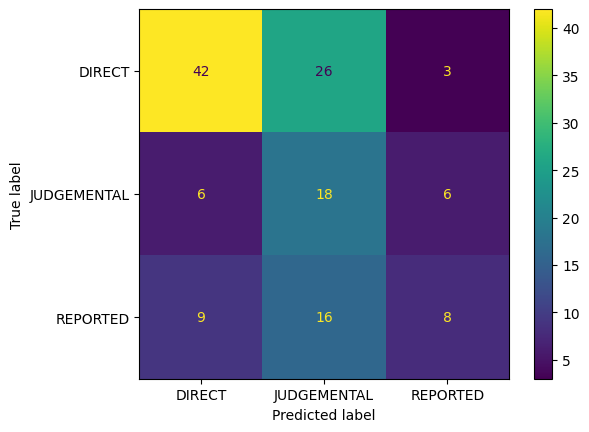
\includegraphics[width=10cm]{imagenes/Evaluacion/confusion_matrix/bert_base-uncased-english-dirty_task2.png}
    \caption{\centering matriz de confusión para bert-base-uncased}
\end{figure}

Para la primera clase se observan un total de 42 instancias bien clasificadas frente al total de 71, es decir un 59.15\%. Por el otro lado las clases Reported y Judgemental tienen 18 y 8 instancias bien clasificadas lo que supone un 60\% y 24.24\% respectivamente. 

Es decir, se puede observar una tendencia por parte del modelo a clasificar hacia la clase Reported con un total de 60 instancias clasificadas como Reported frente a las solo 15 instancias de Judgemental. Esto se puede deber a diversos factores como por ejemplo la hipótesis planteada al inicio sobre la similitud intrínseca de las entradas de tipo Judgemental y de tipo Reported. Es, por tanto, sin duda una tara característica del modelo. Adicionalmente cabe destacar que de manera global el modelo obtiene un 50.7\% de tasa de acierto.


\subsection{Mejores modelos inglés: Twitter\_roberta\_base\_emotion}

A continuación, se ofrecen los resultados para el modelo generado con twitter\_roberta\_base\_emotion, con el cual se desea observar sus valores respecto del modelo  bert\_base-uncased para tratar de determinar si existe alguna causa para esos valores tan dispares.

\begin{table}[H]
\begin{tabular}{|l|c|c|c|c|}
\hline
\rowcolor[HTML]{9B9B9B} 
\multicolumn{1}{|c|}{\cellcolor[HTML]{9B9B9B}{\color[HTML]{000000} \textbf{Versión}}} 
& \multicolumn{1}{l|}{\cellcolor[HTML]{9B9B9B}{\color[HTML]{000000} \textbf{Direct}}} 
& \multicolumn{1}{l|}{\cellcolor[HTML]{9B9B9B}{\color[HTML]{000000} \textbf{Judgemental}}}
& \multicolumn{1}{l|}{\cellcolor[HTML]{9B9B9B}{\color[HTML]{000000} \textbf{Reported}}}
& \multicolumn{1}{l|}{\cellcolor[HTML]{9B9B9B}{\color[HTML]{000000} \textbf{Weighted Average}}} 
\\ \hline
\rowcolor[HTML]{E7E6E6} 
\cellcolor[HTML]{9B9B9B}{\color[HTML]{000000} \textbf{F1}}                           
& {\color[HTML]{000000} 0.66}                                                        
& {\color[HTML]{000000} 0.21}                                                         
& {\color[HTML]{000000} 0.42}                                                         
& {\color[HTML]{000000} 0.50}                                                         
\\ \hline
\rowcolor[HTML]{E7E6E6} 
\cellcolor[HTML]{9B9B9B}{\color[HTML]{000000} \textbf{Precision}}                    
& {\color[HTML]{000000} 0.65}                                                        
& {\color[HTML]{000000} 0.28}                                                        
& {\color[HTML]{000000} 0.36}                                                       
& {\color[HTML]{000000} 0.50}
\\ \hline
\rowcolor[HTML]{E7E6E6} 
\cellcolor[HTML]{9B9B9B}{\color[HTML]{000000} \textbf{Recall}}                       
& {\color[HTML]{000000} 0.66}                                                        
& {\color[HTML]{000000} 0.17}                                                        
& {\color[HTML]{000000} 0.48}                                                         
& {\color[HTML]{000000} 0.51}                                                        
\\ \hline
\end{tabular}
\caption{Métricas segunda tarea para twitter\_roberta\_base\_emotion inglés.}
\end{table}

Una primera vista a los datos sugiere que efectivamente parece que ambos modelos tienen unos resultados similares, al menos en el plano general. Se observan valores muy equilibrados en las diferentes métricas para la clase Direct donde las clases Judgemental y Reported se encuentran significativamente por debajo.

Específicamente se observan unos valores de media de 0.66 para la clase Direct donde Judgemental obtiene para F1, Precision y recall unos valores de 0.21, 0.28 y 0.17 respectivamente. Estos valores se sitúan en la tabla baja comparados con los obtenidos en la clase Reported con 0.42, 0.36 y 0.48 respectivamente.

De manera interesante se observan que los valores medios ponderados son algo bajos comparados con los del modelo anterior salvo para el recall donde este modelo pasa del 0.24 anterior a un 0.50. Con toda esta información se procede a mostrar la matriz de confusión para observar si efectivamente ambos modelos se encuentran prácticamente igual en cuanto a resultados generales como sugieren los datos recién analizados:




\begin{figure}[H]
    \centering
    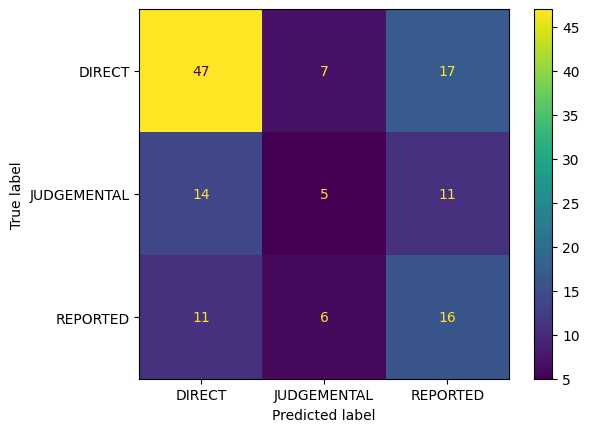
\includegraphics[width=10cm]{imagenes/Evaluacion/confusion_matrix/twitter_roberta_base_emotion-english-dirty_task2.png}
    \caption{\centering matriz de confusión para twitter\_roberta\_base\_emotion inglés}
\end{figure}

Lo primero que se puede observar de manera bastante clara es que el modelo tiene tendencia hacia la clase Direct de manera mayoritaria con un total de 47 instancias del total de 134 donde las siguientes clases son la Judgemental y Reported con un total de 18 y 44 respectivamente. De nuevo se observa esa tendencia a sobre clasificar una de las clases Judgemental o Reported por parte del modelo. En este caso Reported.

Por un lado, la primera clase tiene una tasa de acierto del 66.2\% donde las otras dos clases bajan radicalmente con unos valores del 16.7\% y 48.5\% respectivamente. Sin embargo, pese a estos valores tan bajos para ambas clases el modelo mantiene de manera global unos valores de tasa de acierto casualmente idénticos a los del modelo anterior con un 50.7\%.

Es decir, parece que efectivamente ese valor de loss tan dispar sugería correctamente que existía alguna tara con el modelo bert\_base\_uncased, concretamente parece que estaba sobreentrenado.

\subsection{Modelos bilingües}

A continuación, se realizará el análisis complementario, pero de los cuatro mejores modelos bilingües con el objetivo de determinar de nuevo sus capacidades, características y en general resultados respecto tanto de los modelos en inglés como de los modelos en la primera tarea.


\begin{table}[H]
\begin{tabular}{|l|l|l|l|l|}
\hline
\rowcolor[HTML]{9B9B9B} 
\multicolumn{1}{|c|}{\cellcolor[HTML]{9B9B9B}{\color[HTML]{000000} \textbf{Versión}}}           
& \multicolumn{1}{c|}{\cellcolor[HTML]{9B9B9B}{\color[HTML]{000000} \textbf{Accuracy}}} 
& \multicolumn{1}{c|}{\cellcolor[HTML]{9B9B9B}{\color[HTML]{000000} \textbf{F1}}} 
& \multicolumn{1}{c|}{\cellcolor[HTML]{9B9B9B}{\color[HTML]{000000} \textbf{Precision}}}
& \multicolumn{1}{c|}{\cellcolor[HTML]{9B9B9B}{\color[HTML]{000000} \textbf{Recall}}} 
\\ \hline
\rowcolor[HTML]{E7E6E6} 
\cellcolor[HTML]{9B9B9B}{\color[HTML]{000000} \textbf{bert\_base-cased}}                                                         
& {\color[HTML]{000000} 0.555}                                                     
& {\color[HTML]{000000} 0.463}                                            
& {\color[HTML]{000000} 0.495}                                                    
& {\color[HTML]{000000} 0.496}                                           
\\ \hline
\rowcolor[HTML]{E7E6E6} 
\cellcolor[HTML]{9B9B9B}{\color[HTML]{000000} \textbf{bert\_base\_multilingual-uncased}}                                             
& {\color[HTML]{000000} 0.587}                                                      
& {\color[HTML]{000000} 0.549}                                               
& {\color[HTML]{000000} 0.556}                                                        
& {\color[HTML]{000000} 0.561}                                                   
\\ \hline
\rowcolor[HTML]{E7E6E6} 
\cellcolor[HTML]{9B9B9B}{\color[HTML]{000000} \textbf{twitter\_roberta\_base\_emotion}}                                                   
& {\color[HTML]{000000} 0.590}                                                      
& {\color[HTML]{000000} 0.547}                                                
& {\color[HTML]{000000} 0.552}                                                  
& {\color[HTML]{000000} 0.548}                                                
\\ \hline
\rowcolor[HTML]{E7E6E6} 
\cellcolor[HTML]{9B9B9B}{\color[HTML]{000000} \textbf{XLM\_roBERTa}}                                                                   
& {\color[HTML]{000000} 0.580}                                                    
& {\color[HTML]{000000} 0.537}                                                
& {\color[HTML]{000000} 0.537}                                                  
& {\color[HTML]{000000} 0.548}                                                
\\ \hline
\end{tabular}
\caption{Métricas de los modelos bilingües segunda tarea.}
\end{table}

Lo primero que se puede observar es que los valores de accuracy son claramente inferiores a los de los modelos ingleses con un valor medio alrededor del 57.5\% frente al 60.5\% que mostraban los otros. En general resultados así son de esperar al tratarse de una tarea con mayor complejidad para los modelos de base debido a la mezcla de idiomas, siendo bert un sistema de modelos predominantemente en inglés. Sin embargo, habrá que estudiarlo más en profundidad.

Por un lado el modelo Twitter\_roberta\_base\_emotion aparece de nuevo con un valor de F1  de 0.547 situándose como segundo mejor modelo en esta categoría y con un accuracy del 0.59, en este caso como mejor modelo. En primer lugar, se encuentra el modelo bert\_base\_multilingual-uncased con un valor de F1 realmente similar de 0.549 y lo mismo para su accuracy con un valor de 0.587.

Para esta sección se van a comparar de nuevo dos modelos, concretamente los dos ya mencionados, en este caso por su extrema similitud en las métricas y adicionalmente debido a que el modelo Twitter\_roberta\_base\_emotion sigue siendo una buena comparativa al tratarse del mejor modelo en general hasta el momento durante todo el trabajo.

\subsection{Mejores modelos bilingües: Twitter\_roberta\_base\_emotion}

Estas secciones tienen como objetivo analizar las diferencias entre ambos modelos de tal manera que se puedan observar sus características internas más allá de sus resultados globales. En este caso no hubo ningún resultado anómalo durante el entrenamiento por lo que el estudio se centra en observar su comportamiento.

A continuación, se muestra la tabla con los diferentes resultados y métricas obtenidas:

\begin{table}[H]
\begin{tabular}{|l|c|c|c|c|}
\hline
\rowcolor[HTML]{9B9B9B} 
\multicolumn{1}{|c|}{\cellcolor[HTML]{9B9B9B}{\color[HTML]{000000} \textbf{Versión}}}
& \multicolumn{1}{l|}{\cellcolor[HTML]{9B9B9B}{\color[HTML]{000000} \textbf{Direct}}} 
& \multicolumn{1}{l|}{\cellcolor[HTML]{9B9B9B}{\color[HTML]{000000} \textbf{Judgemental}}} 
& \multicolumn{1}{l|}{\cellcolor[HTML]{9B9B9B}{\color[HTML]{000000} \textbf{Reported}}} 
& \multicolumn{1}{l|}{\cellcolor[HTML]{9B9B9B}{\color[HTML]{000000} \textbf{Average}}} 
\\ \hline
\rowcolor[HTML]{E7E6E6} 
\cellcolor[HTML]{9B9B9B}{\color[HTML]{000000} \textbf{F1}}                          
& {\color[HTML]{000000} 0.75}                                                        
& {\color[HTML]{000000} 0.37}                                                           
& {\color[HTML]{000000} 0.47}                                                           
& {\color[HTML]{000000} 0.60}                                            
\\ \hline
\rowcolor[HTML]{E7E6E6} 
\cellcolor[HTML]{9B9B9B}{\color[HTML]{000000} \textbf{Precision}}       
& {\color[HTML]{000000} 0.70}                                                        
& {\color[HTML]{000000} 0.33}                                                         
& {\color[HTML]{000000} 0.64}                                                           
& {\color[HTML]{000000} 0.62}                                                
\\ \hline
\rowcolor[HTML]{E7E6E6} 
\cellcolor[HTML]{9B9B9B}{\color[HTML]{000000} \textbf{Recall}}             
& {\color[HTML]{000000} 0.80}                                                     
& {\color[HTML]{000000} 0.43}                                                        
& {\color[HTML]{000000} 0.38}                                                           
& {\color[HTML]{000000} 0.61}                                          
\\ \hline
\end{tabular}
\caption{Métricas twitter\_roberta\_base\_emotion bilingüe.}
\end{table}

Inmediatamente se observan unos valores razonablemente buenos para la clase Direct de alrededor del 0.75 para las 3 métricas, lo cual representa los mejores resultados sobre el set de test hasta la fecha. Además, se ha observado que los resultados para las demás clases no son tan radicalmente malos como en los demás modelos con valores de F1, Precision y recall de 0.37, 0.33 y 0.43 respectivamente para Judgemental y de 0.47, 0.64 y 0.38 para Reported. 

A diferencia de en otros modelos, en esta tabla se observa algo más de equilibrio entre las dos clases minoritarias. Este factor puede deberse a que el modelo esta mejor entrenado bien sea por el mayor número de instancias o por el formato del dataset bilingüe.

En total estos resultados brindan alrededor de un 0.6 global de media ponderada para las 3 métricas en el set de test. Este resultado quedará contrastado una vez se realice un breve análisis de la matriz de confusión y se comparen las diferentes accuracy para las 3 clases.


\begin{figure}[H]
    \centering
    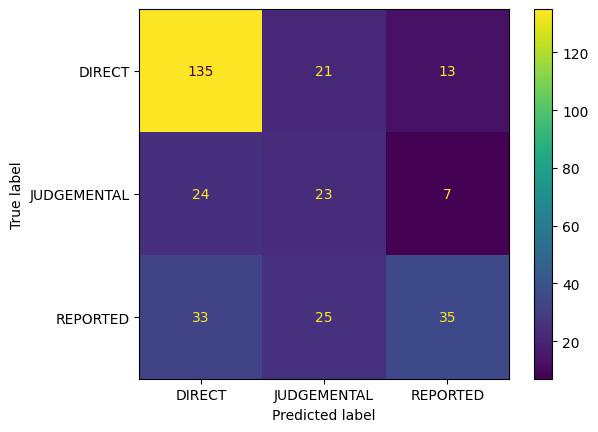
\includegraphics[width=10cm]{imagenes/Evaluacion/confusion_matrix/twitter_roberta_base_emotion-all-dirty.png}
    \caption{\centering matriz de confusión para twitter\_roberta\_base\_emotion bilingüe}
\end{figure}

Para la primera clase se observan buenos resultados con un total de 135 instancias bien clasificadas respecto de un total de 168 (un 80.36\%). Si bien la primera clase obtiene buenos resultados, las otras dos, Judgemental y Reported, no tanto. Por un lado, se tiene Judgemental con 23 instancias bien clasificadas (un 42.6\%) y por otro lado Reported con un total de 35 (un 37.63\%) instancias bien clasificadas.

En general este modelo parece mantener unos buenos resultados, mejores que ningún otro para como mínimo la primera de las clases y para las otras dos clases mantiene unos resultados bajos, pero en la media respecto de los otros modelos. Es decir, en general el modelo obtiene unos valores de accuracy del 61.08\%, siendo por tanto el mejor modelo hasta el momento analizado, aunque solo sea de manera general ya que realmente ese valor surge de los altos resultados para la clase Direct y no tanto para las otras dos clases como ya se ha comentado.


\subsection{Mejores modelos bilingües: Bert\_base\_multilingual-uncased}

Se estudia el siguiente modelo debido a sus resultados obtenidos en la fase previa y como comparativa respecto del modelo anterior. El objetivo es estudiar sus resultados y analizar su comportamiento para ver si se cumplen los mismos patrones que para modelos anteriores.

\begin{table}[H]
\begin{tabular}{|l|c|c|c|c|}
\hline
\rowcolor[HTML]{9B9B9B} 
\multicolumn{1}{|c|}{\cellcolor[HTML]{9B9B9B}{\color[HTML]{000000} \textbf{Versión}}} 
& \multicolumn{1}{l|}{\cellcolor[HTML]{9B9B9B}{\color[HTML]{000000} \textbf{Direct}}}
& \multicolumn{1}{l|}{\cellcolor[HTML]{9B9B9B}{\color[HTML]{000000} \textbf{Judgemental}}}
& \multicolumn{1}{l|}{\cellcolor[HTML]{9B9B9B}{\color[HTML]{000000} \textbf{Reported}}} 
& \multicolumn{1}{l|}{\cellcolor[HTML]{9B9B9B}{\color[HTML]{000000} \textbf{Average}}} 
\\ \hline
\rowcolor[HTML]{E7E6E6} 
\cellcolor[HTML]{9B9B9B}{\color[HTML]{000000} \textbf{F1}}                         
& {\color[HTML]{000000} 0.71 }                                            
& {\color[HTML]{000000} 0.27 }                                                        
& {\color[HTML]{000000} 0.63 }                                                          
& {\color[HTML]{000000} 0.61 }                                             
\\ \hline
\rowcolor[HTML]{E7E6E6} 
\cellcolor[HTML]{9B9B9B}{\color[HTML]{000000} \textbf{Precision}}                  
& {\color[HTML]{000000} 0.74 }                                                        
& {\color[HTML]{000000} 0.26 }                                                       
& {\color[HTML]{000000} 0.60 }                                                         
& {\color[HTML]{000000} 0.62 }                                                
\\ \hline
\rowcolor[HTML]{E7E6E6} 
\cellcolor[HTML]{9B9B9B}{\color[HTML]{000000} \textbf{Recall}}              
& {\color[HTML]{000000} 0.69 }                                                      
& {\color[HTML]{000000} 0.28 }                                                        
& {\color[HTML]{000000} 0.67 }                                                            
& {\color[HTML]{000000} 0.61 }                                                       
\\ \hline
\end{tabular}
\caption{Métricas segunda tarea bert\_base\_multilingual-uncased.}
\end{table}

En primer lugar, se observa de manera clara de nuevo que la clase Direct es la clase con mejores resultados de las 3, sin embargo de manera atípica, la clase Reported no se encuentran lejos con un valor de F1 de 0.63 respecto del 0.71 de la clase Direct.

Por otro lado, la clase Judgemental obtiene unos valores bajísimos para las 3 métricas con 0.27, 0.26 y 0.28 respectivamente para F1, Precision y recall. Esto va en concordancia con la hipótesis de que al ser dos clases muy similares los modelos iban a tener problemas a la hora de diferenciarlas y tenderían a una de las dos como ya se ha observado en anteriores modelos durante el análisis de la tarea 2.

Para poder tener una perspectiva más clara se va a observar la matriz de confusión generada por el modelo:

\begin{figure}[H]
    \centering
    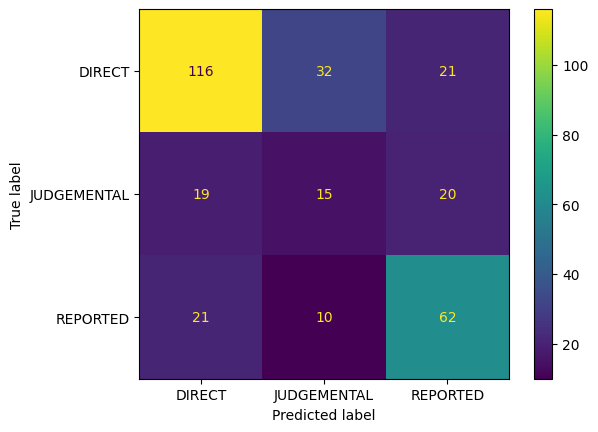
\includegraphics[width=10cm]{imagenes/Evaluacion/confusion_matrix/bert_base_multilingual-uncased-all-dirty_task2.png}
    \caption{\centering matriz de confusión para bert\_base\_multilingual-uncased}
\end{figure}

Como ya se comentaba tanto la clase Direct como la clase Reported obtienen buenos resultados con 116 y 62 instancias correctamente clasificadas para ambas clases frente a las solo 15 de la clase Judgemental.

Es decir, a diferencia del anterior modelo este obtiene valores más bajos para la clase Direct con 116 instancias de 169 (un 68,6\%) pero lo compensa con unos resultados mucho mejores para la clase Reported con 62 instancias de 93 (un 66,6\%) aunque es cierto que para la clase Judgemental cae con un total de 15 instancias de (un 27,7\%).

De nuevo se observa el patrón de clasificación para las dos clases Judgemental y Reported, generando un modelo que tiende a clasificar como una de las dos clases la mayor parte de las instancias de ambas.


\section{Conclusiones modelos}

Finalmente se va a dedicar una sección a cerrar los análisis de ambas tareas determinando que modelos son los mejores y que problemas y limitaciones se han ido encontrando. Si bien se pretende realizar unas conclusiones, estas solo serán sobre los modelos ya que las conclusiones del trabajo se realizarán al final de este.


\subsection{Primera tarea}

En primera instancia se decidió subdividir la tarea en dos versiones, una con un dataset solo con tweets en inglés y otra con todos los tweets (español e inglés), de tal manera que se pudiera observar cuales eran las diferencias entre ambas aproximaciones y ver que alcance tenían los diferentes modelos bert al enfrentarse a una tarea bilingüe.

Además del enfoque por idiomas también se planteó una subdivisión en base al preprocesamiento con el objetivo de observar si aplicar preprocesamiento a los textos mejoraba o empeoraba los resultados finales de los modelos. 

En general y de manera resumida se observó claramente que los modelos con preprocesamiento obtenían peores resultados que aquellos que no estaban preprocesados. Esto se puede deber a diversos factores desde la posibilidad de haber realizado un preprocesamiento que no favorezca si no que perjudique a los modelos hasta la conclusión de que preprocesar los textos hace que el tokenizador no recoja información que de otra manera si recoge y se pierda parte de esa información y por ende de su capacidad de clasificación. Esto se planteará en mejoras futuras.

Como se esperaba la tarea en inglés obtuvo mejores resultados en general convergiendo en el modelo generado con la variante twitter-roberta-base-emotion de roberta para la que se obtuvo un 81.06\% para la tarea 1. Este resultado se sitúa de hecho como el mejor resultado obtenido en todo el trabajo y sería el modelo final si no fuera por su limitación a la hora de trabajar con tweets en español.

Por ello se generó y estudió como ya se comentó una serie de modelos usando el dataset entero con el objetivo de poder realizar la tarea al completo. Para esta tarea se esperaban resultados significativamente peores que los obtenidos para la tarea únicamente inglesa.

Sin embargo, los resultados no son tan malos como se esperaba, convergiendo finalmente en el modelo generado con bert-multilingual-uncased con una tasa de acierto del 77.76\%.

Cabe destacar que si bien ambos modelos generan buenos resultados tienen ambos una tendencia a sobre clasificar hacia la clase No Sexista respecto de la Sexista. Esto probablemente se deba a su el desbalance de los datos del dataset y se deberá plantear en mejoras a futuro.


\subsection{Segunda tarea}

La segunda tarea tenía como objetivo realizar un estudio simplificado de las capacidades de los modelos bert, utilizando como ejemplo los mejores modelos de la anterior tarea. Si bien se sabe que esta aproximación no garantiza los mejores resultados sirve para hacer un estudio de la capacidad de generalizar de esos modelos.

En primera instancia se realizó un estudio con los modelos basados en el dataset en inglés para los que se obtuvieron resultados en general negativos y especialmente para las clases Judgemental y Reported, resultados bastante bajos. específicamente estas dos clases se plantearon de base como una muy probable problemática debido a sus grandes similitudes y discrepancias por parte de los propios anotadores durante todo el dataset. De hecho, se ejemplificó como para un mismo tweet era común encontrar división entre estas dos clases.

Una vez estudiados los diferentes modelos se alcanzó una conclusión sobre ellos, obteniendo para el modelo generado con twitter-roberta-base-emotion una tasa de acierto del 50\%. 

Para la segunda tanda de modelos se esperaba un comportamiento similar a la primera tarea, empeorando de forma ligera los resultados respecto de sus contrapartes en inglés. Sin embargo, los modelos bilingües obtuvieron para las pruebas sobre el test set unos resultados sorprendentemente mejores. Concretamente la tasa de acierto para twitter-roberta-base-emotion y XML-roberta fueron para ambos de un 60\%.

Probablemente estos resultados se deban al reducido tamaño del set de test por lo que con poco los resultados cambian radicalmente y no tanto a un factor de mejor entrenamiento, pero aun así es muy interesante observar cómo su comportamiento difirió completamente de lo esperado para ellos. De nuevo se deberá incluir en mejoras a futuro aumentar el set de test para obtener pruebas con valores más representativos.
\newpage

\chapter{Gestión del proyecto}
El objetivo de este capítulo será realizar una descripción y especificación de todas las características que componen este trabajo desde un punto de vista de la gestión del mismo. Desde la especificación de los requisitos, metodología de desarrollo, planificación y presupuesto. 

\section {Especificación de requisitos}

En el proceso de desarrollo de software, la especificación de requisitos es una etapa fundamental que establece las bases para el diseño y construcción de un sistema o aplicación \cite{mora2007especificacion}. Esta fase tiene como objetivo principal definir de manera clara y concisa tanto los requisitos.

Por un lado, se tienen los funcionales, que describen las funcionalidades específicas que el software debe ofrecer, y por otro lado los no funcionales, que se refieren a aspectos de rendimiento, seguridad, usabilidad y compatibilidadmora2007especificacion \cite{mora2007especificacion}.

A continuación se va a definir el formato en el que se presentarán estos requisitos. Este formato ha sido elegido al ser el más popular y utilizado durante nuestra formación, así como su alta capacidad de síntesis de la información y fácil comprensión. La tabla en cuestión tiene los siguientes campos:

\begin{itemize}
    \item Identificador: Sirve como identificador exclusivo de cada requisito, su formato se compone de los siguiente; RX-N, pudiendo tomar X los valores F (Funcional) o NF (No Funcional) y N como número del requisito dentro de su categoría (F o NF).
    \item Título: Describe de manera concisa el requisito.
    \item Prioridad: Define su nivel de importancia para el proyecto.
    \item Descripción: Describe el requisito de una manera más detallada.
\end{itemize}


\begin{table}[H] 
\begin{center}
\begin{tabular} {|P{4cm}|P{10cm}|}\hline
  \rowcolor{tables} {\bf Identificador} &{\bf RX - N}\\ \hline
  \cellcolor{tables}\textbf{Título}& \\ \hline
  \cellcolor{tables}\textbf{Prioridad}& Alta / Media / Baja  \\ \hline
  \cellcolor{tables}\textbf{Descripción}& \\ \hline
\end{tabular}
\end{center}
\vspace{-0.6cm}
\caption{Plantilla de requisitos}
\end{table}


\subsection {Requisitos Funcionales}
\begin{table}[H] 
\begin{center}
\begin{tabular} {|P{4cm}|P{10cm}|}\hline
  \rowcolor{tables} {\bf Identificador} &{\bf RF - 01}\\ \hline
  \cellcolor{tables}\textbf{Título}& Lectura del dataset\\ \hline
  \cellcolor{tables}\textbf{Prioridad}& Alta \\ \hline
  \cellcolor{tables}\textbf{Descripción}&
  El sistema deberá ser capaz de cargar y leer el dataset para su posterior uso y modificación durante el proyecto. \\ \hline
\end{tabular}
\end{center}
\vspace{-0.6cm}
\caption{Requisito Funcional 01}
\end{table}

\subsection {Requisitos Funcionales}
\begin{table}[H] 
\begin{center}
\begin{tabular} {|P{4cm}|P{10cm}|}\hline
  \rowcolor{tables} {\bf Identificador} &{\bf RF - 02}\\ \hline
  \cellcolor{tables}\textbf{Título}& Análisis de la distribución de clases\\ \hline
  \cellcolor{tables}\textbf{Prioridad}& Alta \\ \hline
  \cellcolor{tables}\textbf{Descripción}& 
  El sistema deberá analizar la distribución de las clases en el dataset para conocer las de mayor frecuencia, siendo las clases 'YES', 'NO' para la clasificación binaria, y 'Direct', 'Reported' y 'Judgmental' para la multi clase como se muestra en la introducción\\ \hline
\end{tabular}
\end{center}
\vspace{-0.6cm}
\caption{Requisito Funcional 02}
\end{table}

\subsection {Requisitos Funcionales}
\begin{table}[H] 
\begin{center}
\begin{tabular} {|P{4cm}|P{10cm}|}\hline
  \rowcolor{tables} {\bf Identificador} &{\bf RF - 03}\\ \hline
  \cellcolor{tables}\textbf{Título}& Procesamiento de la entrada de la tarea 1\\ \hline
  \cellcolor{tables}\textbf{Prioridad}& Alta  \\ \hline
  \cellcolor{tables}\textbf{Descripción}&  Supongamos que las seis anotaciones de un tweet fueron NO ,YES ,NO, YES ,YES ,YES , entonces el valor asignado al tweet será YES. Sin embargo, el número de etiquetas positivas (1 para indicar que el tweet es sexista) y el número de etiquetas negativas (0 para indicar que el tweet no tiene un contenido sexista), entonces se le asignará el valor X, porque es la clase más frecuente en el dataset\\ \hline
\end{tabular}
\end{center}
\vspace{-0.6cm}
\caption{Requisito Funcional 03}
\end{table}


\subsection {Requisitos Funcionales}
\begin{table}[H] 
\begin{center}
\begin{tabular} {|P{4cm}|P{10cm}|}\hline
  \rowcolor{tables} {\bf Identificador} &{\bf RF - 04}\\ \hline
  \cellcolor{tables}\textbf{Título}& Procesamiento de la entrada de la tarea 2\\ \hline
  \cellcolor{tables}\textbf{Prioridad}& Alta  \\ \hline
  \cellcolor{tables}\textbf{Descripción}&  La misma idea que aplicada a la tarea 1 solo que en lugar de elegir entre dos clases se elije entre 3\\ \hline
\end{tabular}
\end{center}
\vspace{-0.6cm}
\caption{Requisito Funcional 04}
\end{table}


\begin{table}[H] 
\begin{center}
\begin{tabular} {|P{4cm}|P{10cm}|}\hline
  \rowcolor{tables} {\bf Identificador} &{\bf RF- 05}\\ \hline
  \cellcolor{tables}\textbf{Título}& Preprocesado de los textos (tweets)\\ \hline
  \cellcolor{tables}\textbf{Prioridad}& Media \\ \hline
  \cellcolor{tables}\textbf{Descripción}& Antes de pasar los textos a nuestros modelos, es necesario procesarlos y transformarlos en vectores. En el preprocesamiento, también se eliminarán ciertas palabras del texto original como las palabras vacías (stop-words), signos de puntuación, números y otros tokens que pueden generar ruido en el entrenamiento del modelo, y que no ayudan en la tarea de clasificación porque no tienen contenido semántico. \\ \hline
\end{tabular}
\end{center}
\vspace{-0.6cm}
\caption{Requisito Funcional 05}
\end{table}

\begin{table}[H] 
\begin{center}
\begin{tabular} {|P{4cm}|P{10cm}|}\hline
  \rowcolor{tables} {\bf Identificador} &{\bf RF- 06}\\ \hline
  \cellcolor{tables}\textbf{Título}& Segmentación estratificada del dataset\\ \hline
  \cellcolor{tables}\textbf{Prioridad}& Alta  \\ \hline
  \cellcolor{tables}\textbf{Descripción}& Para poder entrenar y evaluar nuestros modelos, es necesario crear tres particiones del dataset original para obtener las particiones de training (80\% de los textos), validation (10\%) y test (10\%). Mientras que los dos primeros conjuntos se utilizan para entrenar y ajustar cada modelo, el último se utiliza para proporcionar una evaluación final del modelo. Esta división se realizará de forma aleatoria, pero garantizando que la distribución de clases en cada partición es similar a la del dataset original. \\ \hline
\end{tabular}
\end{center}
\vspace{-0.6cm}
\caption{Requisito Funcional 06}
\end{table}

\begin{table}[H] 
\begin{center}
\begin{tabular} {|P{4cm}|P{10cm}|}\hline
  \rowcolor{tables} {\bf Identificador} &{\bf RF- 07}\\ \hline
  \cellcolor{tables}\textbf{Título}& Tokenización de las entradas\\ \hline
  \cellcolor{tables}\textbf{Prioridad}& Alta  \\ \hline
  \cellcolor{tables}\textbf{Descripción}& Para que el sistema pueda usar los textos es imperativo llevar a cabo una tokenización adecuada de los mismos pasando de valores de texto a tokens, y estos a vectores con un valor asociado dentro de un espacio vectorial, que serán la entrada de nuestros modelos como se cuenta con detalle en la \autoref{tokenización}.\\ \hline
\end{tabular}
\end{center}
\vspace{-0.6cm}
\caption{Requisito Funcional 07}
\end{table}

\begin{table}[H] 
\begin{center}
\begin{tabular} {|P{4cm}|P{10cm}|}\hline
  \rowcolor{tables} {\bf Identificador} &{\bf RF- 08}\\ \hline
  \cellcolor{tables}\textbf{Título}& Entrenamiento y validación de modelos\\ \hline
  \cellcolor{tables}\textbf{Prioridad}& Media\\ \hline
  \cellcolor{tables}\textbf{Descripción}&  El sistema deberá ser capaz de para cada modelo entrenar con el dataset de entrenamiento proporcionado y realizar una posterior validación de los modelos con el dataset de validación\\ \hline
\end{tabular}
\end{center}
\vspace{-0.6cm}
\caption{Requisito Funcional 08}
\end{table}

\begin{table}[H] 
\begin{center}
\begin{tabular} {|P{4cm}|P{10cm}|}\hline
  \rowcolor{tables} {\bf Identificador} &{\bf RF- 09}\\ \hline
  \cellcolor{tables}\textbf{Título}& Clasificación de textos sexistas y no sexistas\\ \hline
  \cellcolor{tables}\textbf{Prioridad}& Alta  \\ \hline
  \cellcolor{tables}\textbf{Descripción}& En la tarea 1, el sistema (es decir, cada uno de los modelos propuestos) deberá inferir para cada texto, si su contenido es sexista.\\ \hline
\end{tabular}
\end{center}
\vspace{-0.6cm}
\caption{Requisito Funcional 09}
\end{table}

\begin{table}[H] 
\begin{center}
\begin{tabular} {|P{4cm}|P{10cm}|}\hline
  \rowcolor{tables} {\bf Identificador} &{\bf RF- 10}\\ \hline
  \cellcolor{tables}\textbf{Título}& Clasificación en la tarea 2\\ \hline
  \cellcolor{tables}\textbf{Prioridad}& Alta  \\ \hline
  \cellcolor{tables}\textbf{Descripción}& En la tarea 2,  el sistema (es decir, cada uno de los modelos propuestos) deberá inferir para cada texto, a qué clase pertenece: direct, Judgmental y reported. Estas clases fueron descritas en detalle en el \autoref{introducción}\\ \hline
\end{tabular}
\end{center}
\vspace{-0.6cm}
\caption{Requisito Funcional 10}
\end{table}

\begin{table}[H] 
\begin{center}
\begin{tabular} {|P{4cm}|P{10cm}|}\hline
  \rowcolor{tables} {\bf Identificador} &{\bf RF- 11}\\ \hline
  \cellcolor{tables}\textbf{Título}& Evaluación\\ \hline
  \cellcolor{tables}\textbf{Prioridad}& Alta  \\ \hline
  \cellcolor{tables}\textbf{Descripción}& Una vez entrenados los modelos, cada uno de ellos debe ser evaluado con las siguientes métricas sobre el conjunto test: Accuracy, Precisión, , Recall, F1 y sus versiones macros.\\ \hline
\end{tabular}
\end{center}
\vspace{-0.6cm}
\caption{Requisito Funcional 11}
\end{table}

\begin{table}[H] 
\begin{center}
\begin{tabular} {|P{4cm}|P{10cm}|}\hline
  \rowcolor{tables} {\bf Identificador} &{\bf RF- 12}\\ \hline
  \cellcolor{tables}\textbf{Título}& Matrices de confusión\\ \hline
  \cellcolor{tables}\textbf{Prioridad}& Alta  \\ \hline
  \cellcolor{tables}\textbf{Descripción}& Además de proporcionar los resultados de cada modelo sobre el conjunto test, el sistema también debe generar la matriz de confusión para cada uno de ellos.\\ \hline
\end{tabular}
\end{center}
\vspace{-0.6cm}
\caption{Requisito Funcional 12}
\end{table}

\subsection {Requisitos No Funcionales}

\begin{table}[H] 
\begin{center}
\begin{tabular} {|P{4cm}|P{10cm}|}\hline
  \rowcolor{tables} {\bf Identificador} &{\bf RNF- 01}\\ \hline
  \cellcolor{tables}\textbf{Título}& Uso de Google Collaboratory\\ \hline
  \cellcolor{tables}\textbf{Prioridad}& Alta \\ \hline
  \cellcolor{tables}\textbf{Descripción}& Se deberán poder usar las diferentes partes que componen al sistema en Google Collaboratory \\ \hline
\end{tabular}
\end{center}
\vspace{-0.6cm}
\caption{Requisito No Funcional 1}
\end{table}


\begin{table}[H] 
\begin{center}
\begin{tabular} {|P{4cm}|P{10cm}|}\hline
  \rowcolor{tables} {\bf Identificador} &{\bf RNF- 02}\\ \hline
  \cellcolor{tables}\textbf{Título}& Código Abierto\\ \hline
  \cellcolor{tables}\textbf{Prioridad}&  Media\\ \hline
  \cellcolor{tables}\textbf{Descripción}& El proyecto deberá ser de libre acceso garantizando el codigo abierto a través de la plataforma \href{https://github.com/ValenUC3M/-NLP-BachelorThesis-GonzaloValenti}{github}\\ \hline
\end{tabular}
\end{center}
\vspace{-0.6cm}
\caption{Requisito No Funcional 2}
\end{table}

\begin{table}[H] 
\begin{center}
\begin{tabular} {|P{4cm}|P{10cm}|}\hline
  \rowcolor{tables} {\bf Identificador} &{\bf RNF- 03}\\ \hline
  \cellcolor{tables}\textbf{Título}& Capacidades de uso\\ \hline
  \cellcolor{tables}\textbf{Prioridad}&  Alta\\ \hline
  \cellcolor{tables}\textbf{Descripción}& El sistema no deberá superar las capacidades ofrecidad por la herramienta Google Collaboratory descrita en la \autoref{entorno}\\ \hline
\end{tabular}
\end{center}
\vspace{-0.6cm}
\caption{Requisito No Funcional 3}
\end{table}

\begin{table}[H] 
\begin{center}
\begin{tabular} {|P{4cm}|P{10cm}|}\hline
  \rowcolor{tables} {\bf Identificador} &{\bf RNF- 04}\\ \hline
  \cellcolor{tables}\textbf{Título}& Python\\ \hline
  \cellcolor{tables}\textbf{Prioridad}&  Alta\\ \hline
  \cellcolor{tables}\textbf{Descripción}& El lenguaje de desarrollo debe ser Python\\ \hline
\end{tabular}
\end{center}
\vspace{-0.6cm}
\caption{Requisito No Funcional 4}
\end{table}


\section{Metodología de desarrollo}

Como ya se ha comentado anteriormente para este trabajo se ha optado por realizar el proceso estándar a la hora de desarrollar un proyecto de software. Como se ha estudiado en el Grado de Ingeniería Informática, la metodología iterativa e incremental conocida como Agile \cite{luna2019usabilidad} es una de las más adecuadas para este proyecto ya que es una metodología que trae consigo múltiples beneficios. Se destaca por su capacidad de adaptarse a los cambios y entregar incrementos de trabajo funcionales de forma continua. Fomenta la colaboración y la comunicación efectivas, así como un enfoque en la calidad y la mejora continua. Además, promueve la transparencia y la visibilidad en todas las etapas del proyecto. En resumen, Agile ofrece flexibilidad, entregas rápidas, colaboración, calidad, mejora constante y transparencia \cite{luna2019usabilidad} que se consideran fundamentales para el correcto desarrollo del proyecto.

De nuevo basándonos en lo aprendido la metodología de desarrollo será iterativa \cite{gutierrez2011metodos}, de tal manera que se siga un orden iterativo de desarrollo pudiendo regresar a anteriores fases del desarrollo para corregir y adaptar el proyecto conforme avance.

El proyecto se ha compuesto de las siguientes fases estándar para un proyecto de desarrollo de software:

\begin{itemize}
    \item Estudio del estado del arte: Estudiar de manera detallada las diferentes tareas asociadas con el proyecto para comprender bien el proceso y obtener posibles ideas y aplicaciones.
    \item Análisis del sistema: Analizar las diferentes características que debe tener el sistema para que funcione correctamente realizando una especificación de los requisitos tanto funcionales como no funcionales.
    \item Desarrollo del sistema: Crear, probar y adaptar un sistema informático capaz de realizar todas las tareas necesarias para realizar el proyecto.
    \item Evaluación del sistema: Una vez generado el sistema se deberá realizar una evaluación de los resultados obtenidos para los diferentes modelos con el objetivo de realizar a posteriori un análisis general de todos los resultados obtenidos.
    \item Desarrollo de la documentación: Para el correcto entendimiento del proyecto y con el objetivo de guardar un registro claro de todo lo requerido para realizar este proyecto se deberá realizar una documentación extensa y detallada que cubra todos los apartados del proyecto ya que la documentación en un proyecto de desarrollo de software es crucial al facilitar la comunicación efectiva entre las partes interesadas, registra las decisiones tomadas, permite el mantenimiento y la escalabilidad del software, facilita la transferencia de conocimiento y asegura el cumplimiento de regulaciones.
\end{itemize}

\section{Planificación del proyecto}

El proyecto se inició el 11 de enero de 2023 y finaliza el 17 de Junio de 2023. En total se han empleado 580 horas para las diferentes fases que han compuesto al proyecto como se muestra a continuación:

\begin{table}[H]
\begin{tabular}{|
>{\columncolor[HTML]{9B9B9B}}c |
>{\columncolor[HTML]{C0C0C0}}c |
>{\columncolor[HTML]{C0C0C0}}c |
>{\columncolor[HTML]{C0C0C0}}c |}
\hline
{\color[HTML]{000000} \textbf{Fases}}           
& \cellcolor[HTML]{9B9B9B}{\color[HTML]{000000} \textbf{Horas}} 
& \cellcolor[HTML]{9B9B9B}{\color[HTML]{000000} \textbf{Fecha de Inicio}}
& \cellcolor[HTML]{9B9B9B}{\color[HTML]{000000} \textbf{Fecha de Fin}} \\ \hline
{\color[HTML]{000000} \textbf{Estado del arte}} 
& {\color[HTML]{000000} 43}                                    
& {\color[HTML]{000000} 11/01/23}                                      
& {\color[HTML]{000000} 27/01/23}                                      
\\ \hline
\textbf{Análisis del sistema}                  
& 96                                                            
& 23/01/23                                                        
& 28/02/23                                                             
\\ \hline
\textbf{Desarrollo del sistema}                
& 207                                                         
& 20/02/23                                                        
& 17/04/23                                                       
\\ \hline
\textbf{Evaluación del sistema}              
& 110                                                       
& 15/04/23                                                        
& 10/05/23                                                       
\\ \hline
\textbf{Documentación}                     
& 167                                                         
& 28/04/23                                                     
& 16/06/23                                                 
\\ \hline
\textbf{Total}                                
& 580                                                          
& 11/01/23                                                        
& 16/06/23                                                         
\\ \hline
\end{tabular}
\caption{Tabla con el tiempo empleado para cada una de las fases del proyecto}
\end{table}

A continuación se muestra el diagrama de GANT para ofrecer una perspectiva visual de la planificación del proyecto:

\begin{figure}[H]
    \centering
    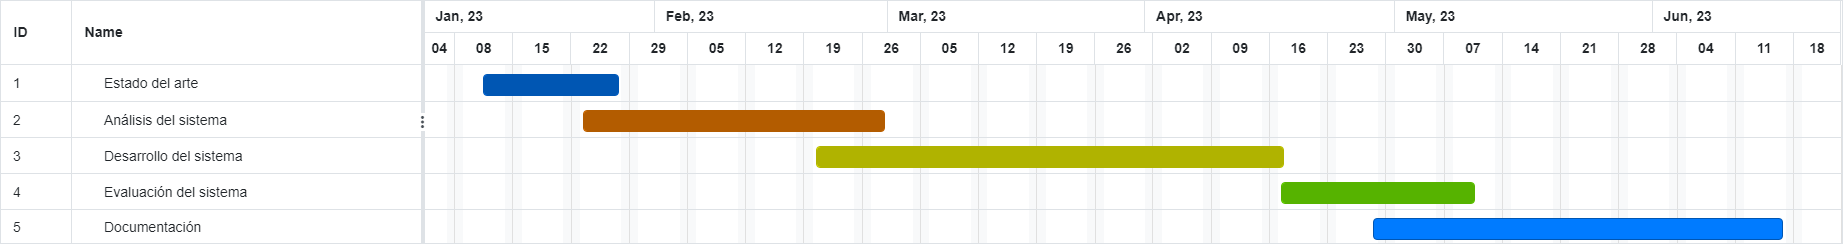
\includegraphics[width=16cm]{imagenes/Gestion/gant.png}
    \caption{\centering diagrama de gant del proyecto}
\end{figure}


\section{Presupuesto y Costes}

En esta sección se presenta el presupuesto del proyecto. Al tratarse de un proyecto individual bajo la supervisión de la tutora Isabel Segura Bedmar, se le asigna el puesto de Técnico de desarrollo a Gonzalo Valenti Sanguino cuya labor es la elaboración del proyecto siguiendo las directivas proporcionadas por su tutora. Dado que el periodo de elaboración del trabajo es del 11 de enero de 2023 al 16 de Julio de 2023 se distribuirán los salarios de manera acorde a esos 5 meses basándonos las \href{https://www.uc3m.es/pdi/media/pdi/doc/archivo/doc_tablas-retributivas-mayo22/tablas-retributivas_contratos-proyectos_30052022.pdf}{tablas retributivas} definidas por el Vicerrectorado el 30 de Mayo de 2022.

Por un lado el sueldo establecido a Isabel Segura es el de Doctor A+ (2.023,81 Euros mensuales) y a Gonzalo Valenti es Especialista C (1.383.33€)


A continuación se muestran la tabla tanto de presupuestos como costes finales asociados al personal del proyecto:

\begin{table}[H]
\begin{tabular}{|c|c|c|c|c|c|}
\hline
\rowcolor[HTML]{9B9B9B} 
\cellcolor[HTML]{9B9B9B}{\color[HTML]{000000} \textbf{Personal}} 
& \cellcolor[HTML]{9B9B9B}{\color[HTML]{000000} \textbf{Sueldo/Hora}} 
& \textbf{Horas/Mes}
& \textbf{Sueldo/Mes}         
& \textbf{Meses} 
& \textbf{Sueldo total}     
\\ \hline
\rowcolor[HTML]{C0C0C0} 
{\color[HTML]{000000} \textbf{Isabel Segura}}                  
& \cellcolor[HTML]{C0C0C0}{\color[HTML]{000000} 11.5€}             
& 30                
& \cellcolor[HTML]{C0C0C0}345€ & 2            
& \cellcolor[HTML]{C0C0C0}690€ \\ \hline
\rowcolor[HTML]{C0C0C0} 
{\color[HTML]{000000} \textbf{Gonzalo Valenti}}              
& {\color[HTML]{000000} 7.86€}                                  
& 116                
& 911,76€                     
& 5             
& 4.558,8€                   
\\ \hline
\end{tabular}
\caption{Tabla de costes asociados al personal del proyecto}
\end{table}

A su vez hay que tener en cuenta los costes asociados las diferentes herramientas de software y hardware usadas durante el proyecto. La herramienta principal es un ordenador de sobremesa custom montado a piezas junto a dos monitores, teclado, ratón y silla, además de una licencia de Windows 10:

\begin{table}[H]
\begin{tabular}{|c|c|}
\hline
\rowcolor[HTML]{9B9B9B} 
{\color[HTML]{000000} \textbf{Descripción}}                   
& {\color[HTML]{000000} \textbf{Coste}}                
\\ \hline
\rowcolor[HTML]{C0C0C0} 
{\color[HTML]{000000} Ordenador sobremesa}                 
& {\color[HTML]{000000} 1079€}                          
\\ \hline
\rowcolor[HTML]{C0C0C0} 
{\color[HTML]{000000} Periféricos}                           
& {\color[HTML]{000000} 212,57€}                     
\\ \hline
\rowcolor[HTML]{C0C0C0} 
\multicolumn{1}{|l|}{\cellcolor[HTML]{C0C0C0} Windows 10 Home} 
& \multicolumn{1}{l|}{\cellcolor[HTML]{C0C0C0} 145€}      
\\ \hline
\rowcolor[HTML]{C0C0C0} 
\multicolumn{1}{|l|}{\cellcolor[HTML]{C0C0C0} Total}         
& \multicolumn{1}{l|}{\cellcolor[HTML]{C0C0C0} 1.436,57€} 
\\ \hline
\end{tabular}
\caption{Coste asociado a las herramientas de hardware y software del proyecto}
\end{table}

Cabe destacar que al ser un ordenador por piezas se ha marcado como referencia para su valor un ordenador equivalente en componentes como el que se muestra en la siguiente referencia \cite{pcomp}.


Adicionalmente se ha usado material de oficina, así como electricidad e internet para poder usar adecuadamente el equipo informático por lo que a continuación se muestra los costes asociados a los mismos:

\begin{table}[H]
\begin{tabular}{|c|c|}
\hline
\rowcolor[HTML]{9B9B9B} 
{\color[HTML]{000000} \textbf{Descripción}}                   
& {\color[HTML]{000000} \textbf{Coste}}                
\\ \hline
\rowcolor[HTML]{C0C0C0} 
{\color[HTML]{000000} Material de oficina}                 
& {\color[HTML]{000000} 45€}                          
\\ \hline
\rowcolor[HTML]{C0C0C0} 
{\color[HTML]{000000} Electricidad}                           
& {\color[HTML]{000000} 385€}                     
\\ \hline
\rowcolor[HTML]{C0C0C0} 
\multicolumn{1}{|l|}{\cellcolor[HTML]{C0C0C0} Internet} 
& \multicolumn{1}{l|}{\cellcolor[HTML]{C0C0C0} 57,90€}      
\\ \hline
\rowcolor[HTML]{C0C0C0} 
\multicolumn{1}{|l|}{\cellcolor[HTML]{C0C0C0} Total}         
& \multicolumn{1}{l|}{\cellcolor[HTML]{C0C0C0} 487,90€} 
\\ \hline
\end{tabular}
\caption{Coste indirectos}
\end{table}

Al tratarse de proyecto de investigación sin ánimo de lucro los beneficios son nulos por lo que el desglose de costes finales queda de la siguiente manera:

\begin{table}[H]
\begin{tabular}{|c|c|}
\hline
\rowcolor[HTML]{9B9B9B} 
{\color[HTML]{000000} \textbf{Descripción}}                   
& {\color[HTML]{000000} \textbf{Coste}}                
\\ \hline
\rowcolor[HTML]{C0C0C0} 
{\color[HTML]{000000} Personal}                 
& {\color[HTML]{000000} 5.248,8€}                          
\\ \hline
\rowcolor[HTML]{C0C0C0} 
{\color[HTML]{000000} Hardware y Software}                           
& {\color[HTML]{000000} 1.436,57€}                     
\\ \hline
\rowcolor[HTML]{C0C0C0} 
\multicolumn{1}{|l|}{\cellcolor[HTML]{C0C0C0}Material} 
& \multicolumn{1}{l|}{\cellcolor[HTML]{C0C0C0}487,90€}      
\\ \hline
\rowcolor[HTML]{C0C0C0} 
\multicolumn{1}{|l|}{\cellcolor[HTML]{C0C0C0}Total}         
& \multicolumn{1}{l|}{\cellcolor[HTML]{C0C0C0}7.173,27€} 
\\ \hline
\end{tabular}
\caption{Coste asociado a las herramientas de hardware y software del proyecto}
\end{table}
\newpage

\chapter{Impacto socieconómico y marco legislativo}

\section{Impacto}
La detección de sexismo en la sociedad es un tema de gran importancia en la actualidad, ya que el sexismo es un problema social que puede tener consecuencias negativas en la vida de las personas. La inteligencia artificial (IA) y en particular el procesamiento del lenguaje natural (PLN), han demostrado ser herramientas valiosas para detectar el sexismo en el lenguaje utilizado en diferentes contextos, como en redes sociales, textos de noticias \cite{mosqueda2023uso}, anuncios publicitarios \cite{villanueva2013autodependencia}, entre otros.

Un ejemplo concreto de aplicación del NLP para la detección de sexismo en el lenguaje es el análisis de las redes sociales. Las redes sociales son una fuente valiosa de datos para los investigadores que buscan analizar los patrones de lenguaje y comportamiento en línea. El análisis de las redes sociales con herramientas basadas en NLP puede permitir la identificación de patrones discriminatorios en el lenguaje utilizado en las publicaciones, los comentarios y las conversaciones en línea \cite{racca2022deteccion}.

La detección de sexismo basada en NLP también puede ser utilizada en la educación y la concientización sobre el sexismo en la sociedad. Los programas de educación \cite{calero2021modelo} y concienciación pueden utilizar el análisis de patrones discriminatorios en el lenguaje para enseñar a los estudiantes sobre los estereotipos de género y los roles tradicionales de género \cite{azpillaga2021analisis}. También se pueden utilizar herramientas de detección de sexismo basadas en NLP para evaluar la efectividad de los programas de educación y concientización sobre el sexismo.

En conclusión de cara al impacto, el uso de NLP para la detección de sexismo en la sociedad es una herramienta valiosa para combatir el sexismo en el lenguaje y en la cultura en general. Con el desarrollo continuo de las herramientas de NLP y la inteligencia artificial en general, es probable que la detección de sexismo en la sociedad siga mejorando en el futuro.

\section{Legislación}
Desde una perspectiva legislativa y legal, hay varios marcos regulatorios que buscan garantizar que la aplicación de la inteligencia artificial (IA) no viole ninguna ley fundamental y que se respeten los derechos de la sociedad.

En la Unión Europea, por ejemplo, se ha establecido el Reglamento General de Protección de Datos (RGPD \cite{de2016reglamento}), que establece las normas para la recopilación, el procesamiento y el almacenamiento de datos personales. El RGPD establece que cualquier uso de datos personales debe ser justo, transparente y basado en el consentimiento del usuario, y que los usuarios tienen derecho a solicitar que se borren sus datos personales en cualquier momento. Además, la UE está trabajando en un marco regulador específico para la IA \cite{EU-IA} , que se espera que establezca directrices sobre la transparencia y la responsabilidad en la toma de decisiones automatizada.

Por otro lado, España no se queda en absoluto atrás. A efectos de la ley desde el 13 de Julio de 2022 se estableció la ley integral para la igualdad de trato y la no discriminación \cite{leyespanola}. La cual establece que cualquier decisión basada en IA deberá ser auditable, revisable y controvertible por la decisión humana así como garantizar que su uso será en pos del bien común sin tener ningun otro objetivo que no sea ese. Si bien esta ultima linea es algo genérica, cada vez más la ley está garantizando el uso responsable y adecuado de la IA en nuestra sociedad.

Desde una perspectiva legislativa, en conclusión, existen marcos legales y regulatorios que buscan garantizar que la aplicación de la IA respete los derechos de la sociedad y no viole ninguna ley fundamental. Es importante que se sigan desarrollando y actualizando estos marcos para garantizar que la tecnología se utilice de manera ética y responsable.
\newpage

\chapter{Conclusiones y trabajo futuro}
Este capítulo tiene como objetivo realizar una revisión de todo el trabajo presentando las principales conclusiones, problemas encontrados durante la realización del mismo, así como aplicaciones a futuro para mejorar el estudio.

Para este trabajo se han utilizado diferentes modelos generados con Transformers para la tarea de detección de sexismo en redes sociales, y la subtarea de clasificación multi clase de intención para cada mensaje sexista. El dataset para este estudio, así como la idea de las tareas se ha obtenido de la competición EXIST 2023 \cite{EXIST2023}.

Para abordar estas tareas se han escogido una serie de modelos: BERT, con las variantes cased y uncased además de la variante multilingual, RoBERTa con las variantes base y twitter\_roberta\_base\_emotion y por último XLM-RoBERTa con las variantes base y large, aunque esta última no se ha podido usar por limitaciones del entorno de desarrollo ya mencionadas.

Además de abordar la tarea considerando únicamente los tweets escritos en inglés, y por otro lado, toda la colección de tweets (que también incluía tweets escritos en español),  también se realizó un preprocesado de los tweets para poder realizar una comparativa de resultados de preprocesados y no preprocesados por lo que en total se obtuvieron cuatro datasets. En el preprocesado, se incluyeron tareas para la limpieza de los tweets (eliminar palabras de paradas, signos de puntuación, etc). 

El objetivo del análisis era observar en primer lugar, los efectos del preprocesamiento y en segundo lugar la capacidad de los modelos transformadores de detectar el sexismo tanto en inglés (al ser el idioma principal usado en estos) como en una tarea donde se enfrentaran tanto al inglés como a un idioma adicional (en este caso el español). Es por eso que no se usaron modelos específicos para el español si no que se abordó la tarea desde una perspectiva multilingüe.

Los resultados obtenidos fueron los siguientes:

\begin{itemize}
    \item Tarea 1: El mejor modelo para los tweets solo en inglés fue el generado con twitter\_roberta\_base\_emotion y por otro lado, para la tarea en su formato multilingüe el mejor modelo fue Bert multilingüe uncased.
    \item Tarea 2: El mejor modelo para los tweets escritos en inglés fue de nuevo el generado con twitter\_roberta\_base\_emotion obteniendo un valor donde para la tarea multilingüe el mejor modelo fue también de nuevo Bert\_base\_multilingual-uncased.
\end{itemize}

El principal problema encontrado durante el trabajo ha sido el alcance de este, si bien se querían realizar pruebas usando más modelos transformadores y también un apartado específico para los tweets en español por limitaciones de tiempo se tuvo que determinar reducir el alcance del mismo. Es por eso que se plantea a futuro usar más modelos como ROBERTuito , distilBERT, Beto, BERTweet y la variante de RoBERTa twitter-roberta-base no especifica para análisis de sentimiento.

De nuevo desde la perspectiva de la limitación temporal se decidió centrarse en el estudio de la clasificación de sexismo y detección de intenciones dejando a un lado la tercera tarea planteada por EXIST 2023 de subclasificación de sexismo en subtipos. Esta tarea es muy interesante y se plantea su estudio para futuras aproximaciones.

En lo que respecta a los modelos y las tareas, otro de los retos fue el tratamiento de la información proporcionada por los seis anotadores que etiquetaron los tweets (es decir, cada tweets estaba anotado con seis etiquetas distintas para cada tarea), si bien se decidió simplificar esas entradas a una única anotación (seleccionando la anotación más frecuente entre los anotadores), en lugar de explotar las seis anotaciones para cada tweet. Sería interesante a futuro analizar distintas alternativas al problema y estudiar sus resultados. Por ejemplo, en lugar de seleccionar la anotación más frecuente, un posible enfoque sería ponderar las anotaciones de los anotadores según el sexo y edad de los anotadores (en el análisis de datos, se ha estudiado que podría existir un pequeño posible sesgo en la anotación dependiendo de la edad y género del anotador). 

Finalmente, de cara a las limitaciones, desde una perspectiva de los recursos, una de las más significativas fue el uso de la plataforma Google Colab, con frecuencia tras realizar un número de pruebas, la plataforma suele bloquear el acceso a la GPU por un abuso del uso de esta. Esto se podría haber solucionado con acceso a la versión de pago de la plataforma (Google Colab Pro), y se plantea como una medida necesaria si se desea estudiar en profundidad las diferentes problemáticas ya planteadas.

Desde una perspectiva personal este trabajo ha supuesto un reto mayor sin precedentes, no solo porque nunca  había realizado un análisis de un conjunto de datos de este tamaño y con esta estructura, sino también por el desconocimiento general de las herramientas en materia de PLN. Esto ha provocado sin duda retrasos en las distintas fases del proyecto, así como tomas de decisiones que en resumen han perjudicado a la calidad del estudio. Dicho eso, actualmente considero que he adquirido los conocimientos y experiencia necesarios para abordar el desarrollo de sistemas para aplicaciones de PLN basados en enfoques de aprendizaje profundo, y en particular, con transformadores. 
\newpage



%----------
%	BIBLIOGRAFÍA
%----------	

% \nocite{*} % Si quieres que aparezcan en la bibliografía todos los documentos que la componen (también los que no estén citados en el texto) descomenta está lína

\clearpage
\addcontentsline{toc}{chapter}{Bibliografía}
%\setquotestyle[english]{british} % Cambiamos el tipo de cita porque en el estilo IEEE se usan las comillas inglesas.
\printbibliography

\end{document}
